\documentclass[12pt,a4paper,oneside,openany]{book}
\usepackage{styles/uet-report}
\usepackage{amsmath,amssymb}
\usepackage{array}
\usepackage{booktabs}
\usepackage{longtable}
\usepackage{pdflscape}

\newcommand{\reporttitle}{NGHIÊN CỨU VÀ THỰC NGHIỆM MÔ HÌNH DỰ BÁO TIÊU THỤ NĂNG LƯỢNG\\KẾT HỢP FEATURE SELECTION VÀ INTERPRETABLE MACHINE LEARNING}
\newcommand{\reporttype}{BÁO CÁO GIỮA KỲ}
\newcommand{\coursename}{Phân tích dữ liệu dự báo}
\newcommand{\studentname}{NGUYỄN THÁI SƠN}
\newcommand{\majorname}{Hệ thống thông tin}
\newcommand{\lecturername}{TS.Nguyễn Thị Hậu}
\newcommand{\reportyear}{2026}

\begin{document}
\selectlanguage{vietnamese}
\hypersetup{pageanchor=false}
% Trang bia theo project mau UET; noi dung lay nguyen tu file Word.
\begin{titlepage}
\thispagestyle{empty}
\begin{tikzpicture}[remember picture,overlay]
    \draw[line width=1.1pt]
      ([xshift=1.45cm,yshift=-1.45cm]current page.north west)
      rectangle
      ([xshift=-1.45cm,yshift=1.45cm]current page.south east);
    \draw[line width=0.45pt]
      ([xshift=1.56cm,yshift=-1.56cm]current page.north west)
      rectangle
      ([xshift=-1.56cm,yshift=1.56cm]current page.south east);
\end{tikzpicture}
\begin{center}
\vspace*{1.2cm}
{\fontsize{16}{20}\selectfont ĐẠI HỌC QUỐC GIA HÀ NỘI\par}
\vspace{0.15cm}
{\bfseries\fontsize{16}{20}\selectfont TRƯỜNG ĐẠI HỌC CÔNG NGHỆ\par}
\vspace{1.0cm}

\includegraphics[width=3.5cm]{uet-logo.png}\par
\vspace{0.6cm}
{\bfseries\fontsize{17}{21}\selectfont \studentname\par}
\vspace{1.0cm}
{\bfseries\fontsize{21}{27}\selectfont \reporttitle\par}
\vspace{1.0cm}
{\bfseries\fontsize{15.5}{19}\selectfont \reporttype\par}
\vspace{0.15cm}
{\fontsize{13.5}{17}\selectfont Môn: \coursename\par}
\vspace{0.25cm}
{\fontsize{13.5}{17}\selectfont Ngành: \majorname\par}
\vspace{0.25cm}
{\fontsize{13.5}{17}\selectfont Giảng viên hướng dẫn: \lecturername\par}
\vfill
{\bfseries\fontsize{14.5}{18}\selectfont HÀ NỘI - \reportyear\par}
\vspace*{1.0cm}
\end{center}
\end{titlepage}

\hypersetup{pageanchor=true}

\frontmatter
\chapter*{Tóm tắt}
\thispagestyle{plain}
\addcontentsline{toc}{chapter}{Tóm tắt}

Báo cáo nghiên cứu và tái triển khai framework dự báo tiêu thụ năng lượng được đề xuất bởi Eskandari và cộng sự (2024), trong đó Feature Selection được kết hợp với năm mô hình học máy và SHAP nhằm đồng thời xem xét độ chính xác, tính gọn của tập biến và khả năng diễn giải. Thay vì sử dụng dữ liệu tiêu thụ năng lượng quốc gia theo tháng của Vương quốc Anh như nghiên cứu gốc, thực nghiệm này ánh xạ framework sang bộ dữ liệu Appliances Energy Prediction (KAG\_energydata\_complete.csv), gồm 19.735 quan sát được ghi nhận mỗi 10 phút tại một ngôi nhà hiệu quả năng lượng ở Bỉ. Bài toán được thiết kế thành dự báo một bước: sử dụng thông tin tại thời điểm t để dự báo Appliances tại thời điểm t+1, tương ứng 10 phút.

Quy trình gồm kiểm tra chất lượng dữ liệu, xây dựng biến thời gian chu kỳ, chia dữ liệu theo thời gian với tỷ lệ 80/20, chuẩn hóa chỉ trên tập huấn luyện, bốn base feature selectors (mRMR, Random Forest, RReliefF và F-test FS), ba nhánh lựa chọn S1, S2 và S1S2, Bayesian Optimization, năm mô hình LASSO, SVR-Linear, SVR-RBF, GPR và LSBoost, cùng phân tích SHAP. Trong 20 cấu hình dự báo đã lưu, tất cả đều có trạng thái `ok`. Cấu hình S1-LSBoost đạt RMSE 61,224 Wh, MAE 26,544 Wh và R² = 0,5477, đứng đầu theo RMSE trên holdout test. S1 sử dụng 10/36 đặc trưng; trong khi S2 và S1S2 đều chọn duy nhất Appliances\_t cho cả năm estimator. Các baseline bổ sung gồm Persistence, Ridge, RandomForest và HistGradient\allowbreak Boosting.

Hai thí nghiệm mở rộng đã được thực hiện và lưu kết quả. Lag Feature Ablation cho thấy khi loại Appliances\_t khỏi tập S1 đã chọn (từ 10 xuống 9 đặc trưng), RMSE của LSBoost tăng 40,41\%, từ 61,224 lên 85,967 Wh. Trong Gaussian Noise Robustness, RMSE trung bình tăng lần lượt 20,67\%, 50,80\% và 103,62\% tại các mức độ lệch chuẩn nhiễu 0,05; 0,10 và 0,20 trên không gian đặc trưng đã MinMax scaling. Các kết quả cho thấy giá trị hiện tại của tiêu thụ điện chứa thông tin dự báo rất mạnh đối với chân trời 10 phút, đồng thời mô hình S1-LSBoost nhạy với nhiễu đầu vào.

Đây là method reproduction trên một dataset khác, không phải replication trực tiếp dữ liệu và trị số của bài báo gốc. Những khác biệt quan trọng gồm miền dữ liệu và tần suất, ánh xạ Relief sang RReliefF cho hồi quy, Python port của SIFE sử dụng Jaccard distance như proxy cho fuzzy granulation, ánh xạ MATLAB models sang scikit-learn, giới hạn mẫu tính toán và Permutation\allowbreak Explainer với ngân sách hữu hạn. Vì vậy, báo cáo chỉ kết luận trong phạm vi bộ dữ liệu KAG và cấu hình thực nghiệm đã chạy; không diễn giải các metric KAG như kết quả so sánh trực tiếp với Table 7 của bài báo.

\emph{Từ khóa: Energy consumption forecasting; Feature Selection; Ensemble filter; SIFE; SHAP; LSBoost; KAG Appliances Energy Prediction.}
\clearpage

\tableofcontents
\clearpage
\chapter*{Danh sách thuật ngữ và ký hiệu}
\addcontentsline{toc}{chapter}{Danh sách thuật ngữ và ký hiệu}
\small
\begin{longtable}[]{@{}
  >{\raggedright\arraybackslash}p{(\columnwidth - 4\tabcolsep) * \real{0.3333}}
  >{\raggedright\arraybackslash}p{(\columnwidth - 4\tabcolsep) * \real{0.3333}}
  >{\raggedright\arraybackslash}p{(\columnwidth - 4\tabcolsep) * \real{0.3333}}@{}}
\toprule\noalign{}
\begin{minipage}[b]{\linewidth}\raggedright
\textbf{Ký hiệu}
\end{minipage} & \begin{minipage}[b]{\linewidth}\raggedright
\textbf{Tên tiếng Anh}
\end{minipage} & \begin{minipage}[b]{\linewidth}\raggedright
\textbf{Diễn giải}
\end{minipage} \\
\midrule\noalign{}
\endhead
\bottomrule\noalign{}
\endlastfoot
EC & Energy Consumption & Tiêu thụ năng lượng \\
FS & Feature Selection & Lựa chọn đặc trưng \\
ML & Machine Learning & Học máy \\
SHAP & Shapley Additive Explanations & Giải thích dựa trên giá trị Shapley \\
S0 & Initial feature set & Tập đặc trưng ban đầu \\
S1 & Ensemble filter & Tập chọn bằng lọc tổ hợp \\
S2 & Wrapper & Tập chọn bằng phương pháp bao \\
S1S2 & Ensemble filter-wrapper & Tập chọn lai lọc--bao \\
SIFE & Set-based Integer-coded Fuzzy granular Evolutionary & Thuật toán tiến hóa SIFE \\
mRMR & Maximum Relevance Minimum Redundancy & Tối đa liên quan, tối thiểu dư thừa \\
RReliefF & Regression ReliefF & Biến thể Relief cho hồi quy \\
GPR & Gaussian Process Regression & Hồi quy quá trình Gaussian \\
SVR & Support Vector Regression & Hồi quy vector hỗ trợ \\
LSBoost & Least-Squares Gradient Tree Boosting & Tăng cường cây theo bình phương tối thiểu \\
RMSE & Root Mean Squared Error & Căn sai số bình phương trung bình \\
MAE & Mean Absolute Error & Sai số tuyệt đối trung bình \\
MAPE & Mean Absolute Percentage Error & Sai số phần trăm tuyệt đối trung bình \\
R² & Coefficient of determination & Hệ số xác định \\
IQR & Interquartile Range & Khoảng tứ phân vị \\
MCAR & Missing Completely At Random & Thiếu hoàn toàn ngẫu nhiên \\
BO & Bayesian Optimization & Tối ưu Bayes \\
\end{longtable}
\normalsize
\clearpage

\listoffigures
\addcontentsline{toc}{chapter}{Danh sách hình vẽ}
\listoftables
\addcontentsline{toc}{chapter}{Danh sách bảng}

\mainmatter
\pagestyle{plain}
\chapter*{MỞ ĐẦU}
\addcontentsline{toc}{chapter}{MỞ ĐẦU}
\label{chap:mo-dau}

Dự báo tiêu thụ năng lượng có vai trò quan trọng trong quản lý tòa nhà, điều phối phụ tải, lập kế hoạch vận hành và đánh giá hiệu quả sử dụng năng lượng. Ở cấp độ một hộ gia đình hoặc một công trình, chuỗi tiêu thụ có thể biến động theo lịch sinh hoạt, hoạt động của thiết bị, ánh sáng, nhiệt độ và độ ẩm. Dữ liệu cảm biến hiện đại cho phép quan sát đồng thời nhiều biến, nhưng cũng làm xuất hiện câu hỏi về việc chọn biến nào, mô hình nào phù hợp và làm thế nào để diễn giải đóng góp của các biến đầu vào.

Eskandari và cộng sự (2024) đề xuất một framework tích hợp ba hướng Feature Selection (ensemble filter, wrapper và hybrid ensemble filter-wrapper), năm mô hình học máy và SHAP. Điểm đáng chú ý của nghiên cứu không nằm ở một estimator đơn lẻ mà ở việc đặt lựa chọn đặc trưng và mô hình dự báo trong một quy trình so sánh có hệ thống. Bài báo hướng tới dự báo tiêu thụ năng lượng quốc gia của Vương quốc Anh với dữ liệu theo tháng, đồng thời tìm một thỏa hiệp giữa độ chính xác và số lượng biến cần thiết {[}1{]}.

Báo cáo này tái triển khai framework trên bộ Appliances Energy Prediction của UCI, là dữ liệu cảm biến tại một ngôi nhà hiệu quả năng lượng ở Bỉ. Do khác biệt về miền dữ liệu, tần suất, target, danh sách biến và nền tảng triển khai, công việc được xác định là method reproduction trên dữ liệu khác, không phải replication định lượng trực tiếp. Sự phân biệt này được duy trì xuyên suốt báo cáo: phần lý thuyết mô tả phương pháp bài báo; phần triển khai mô tả đúng code ABC-1.2; phần kết quả chỉ trình bày những gì đã được notebook ghi nhận.

Nội dung báo cáo được tổ chức thành sáu chương theo cấu trúc báo cáo mẫu và có bổ sung một chương riêng để trình bày kết quả do tác giả nghiên cứu gốc công bố. Chương 1 giới thiệu bài toán và nghiên cứu gốc; Chương 2 phân tích cơ sở lý thuyết và lý do kết hợp các phương pháp; Chương 3 mô tả dữ liệu, môi trường và giao thức thực nghiệm; Chương 4 trình bày kết quả tái triển khai trên KAG gồm 20 cấu hình forecasting, baseline, SHAP và hai thí nghiệm mở rộng; Chương 5 trình bày riêng kết quả thực nghiệm được công bố trong bài báo gốc để làm mốc tham chiếu; Chương 6 tổng kết kết quả, giới hạn và hướng phát triển. Hình xuất từ notebook và hình/bảng trích từ bài báo được tách thành các phụ lục riêng, có ghi rõ nguồn.

\chapter{Giới thiệu đề tài}\label{chap:7}

\section{Bối cảnh và chủ đề nghiên cứu}\label{bux1ed1i-cux1ea3nh-vuxe0-chux1ee7-ux111ux1ec1-nghiuxean-cux1ee9u}

Nhu cầu dự báo năng lượng xuất hiện ở nhiều cấp độ: thiết bị, hộ gia đình, tòa nhà, ngành kinh tế và hệ thống năng lượng quốc gia. Ở cấp độ công trình, dữ liệu được ghi nhận với tần suất cao và gắn với cảm biến nhiệt độ, độ ẩm, chiếu sáng cùng dữ liệu thời tiết. Đặc điểm này giúp xây dựng các mô hình dự báo ngắn hạn, nhưng đồng thời làm tăng số lượng biến và nguy cơ đa cộng tuyến, dư thừa thông tin hoặc phụ thuộc quá mức vào một số biến trễ.

Các mô hình hồi quy tuyến tính thường dễ diễn giải nhưng có thể không mô tả đầy đủ quan hệ phi tuyến. SVR với kernel RBF, GPR và LSBoost cung cấp khả năng mô hình hóa linh hoạt hơn, tuy nhiên tính phức tạp tăng lên và việc giải thích vai trò của từng biến trở nên quan trọng. Vì vậy, feature selection và explainable machine learning có thể được xem như hai thành phần bổ sung: thành phần thứ nhất giảm chiều đầu vào, thành phần thứ hai diễn giải dự báo sau khi mô hình được huấn luyện.

\section{Phát biểu bài toán}\label{phuxe1t-biux1ec3u-buxe0i-touxe1n}

Cho chuỗi quan sát tại các thời điểm cách nhau 10 phút. Tại thời điểm $t$, vector đặc trưng gồm các biến cảm biến, thời tiết, chiếu sáng, đặc trưng thời gian và mức tiêu thụ \texttt{Appliances} tại thời điểm hiện tại. Mục tiêu là dự báo mức tiêu thụ \texttt{Appliances} tại bản ghi kế tiếp:

\begin{equation}
    \hat{y}(t+1) = f_{\theta}(x(t)),
    \quad x(t) \in \mathbb{R}^{36},
    \quad \hat{y}(t+1) \in \mathbb{R}.
    \label{eq:forecast}
\end{equation}

Trong đó, $\hat{y}(t+1)$ được ánh xạ từ cột
\texttt{Appliances\_t\_plus\_1}; tần suất dữ liệu đều 10 phút nên
horizon one-step bằng 10 phút. Đây là dự báo điểm cho một thời điểm
tương lai, không phải dự báo multi-horizon $H$-step như một số bài toán
forecasting dài hạn.

\section{Thách thức của bài toán}\label{thuxe1ch-thux1ee9c-cux1ee7a-buxe0i-touxe1n}

Thứ nhất, các biến cảm biến có thang đo và tính chất khác nhau. Nhiệt độ, độ ẩm, áp suất, tốc độ gió, ánh sáng và năng lượng không thể so sánh trực tiếp nếu không chuẩn hóa. Việc fit scaler trên toàn bộ dữ liệu cũng có thể làm rò rỉ thông tin từ giai đoạn test, do đó notebook chỉ fit \texttt{MinMaxScaler} trên tập \texttt{train}.

Thứ hai, thời gian có cấu trúc chu kỳ và tự tương quan. Giá trị tiêu thụ ở thời điểm gần nhất thường mang thông tin mạnh về mười phút tiếp theo. Nếu không kiểm soát, mô hình có thể đạt kết quả tốt chủ yếu nhờ lag target, thay vì khai thác các biến môi trường. Đặc điểm này trở thành vấn đề quan trọng khi \texttt{S2} và \texttt{S1S2} chỉ chọn \texttt{Appliances\_t}.

Thứ ba, feature selection có đánh đổi giữa tốc độ và tính gắn với estimator. Filter đánh giá đặc trưng tương đối độc lập với mô hình; wrapper tìm tập biến dựa trên hiệu năng của estimator nhưng chi phí cao; hybrid dùng filter để rút gọn không gian tìm kiếm trước khi wrapper tối ưu.

Thứ tư, nhiều biến cảm biến có tương quan, khiến importance và SHAP có thể phân bổ ảnh hưởng không ổn định giữa các biến thay thế.

Thứ năm, việc tái hiện một framework trên dataset khác đòi hỏi ánh xạ thuật toán và công cụ. Khác biệt giữa MATLAB và scikit-learn, cũng như giới hạn tính toán khi chạy wrapper trên dữ liệu tần suất cao, có thể làm kết quả khác bài báo gốc. Các khác biệt này cần được định lượng và ghi nhận thay vì che giấu.

\section{Bài báo gốc và những đóng góp chính}\label{buxe0i-buxe1o-gux1ed1c-vuxe0-nhux1eefng-ux111uxf3ng-guxf3p-chuxednh}

Bài báo tham chiếu là ``Innovative framework for accurate and transparent forecasting of energy consumption: A fusion of feature selection and interpretable machine learning'' của Eskandari, Saadatmand, Ramzan và Mousapour, xuất bản trên Applied Energy, tập 366, năm 2024, số bài 123314, DOI 10.1016/j.apenergy.2024.123314 [1]. Nghiên cứu xây dựng framework dự báo tiêu thụ năng lượng cuối cùng tổng hợp ở cấp quốc gia tại Vương quốc Anh, sử dụng các biến liên quan đến năng lượng, kinh tế-xã hội, dân số, khí tượng và thời gian. Bài báo nhấn mạnh ba đóng góp phương pháp: ensemble filter mới, so sánh có hệ thống ba chiến lược feature selection với năm estimator, và sử dụng SHAP cho mô hình có hiệu năng cao [1].

\begin{small}
\begin{longtable}{
    @{}
    >{\raggedright\arraybackslash}p{0.18\textwidth}
    >{\raggedright\arraybackslash}p{0.31\textwidth}
    >{\raggedright\arraybackslash}p{0.40\textwidth}
    @{}
}
\caption{Đối chiếu mục tiêu và nội dung bài báo tham chiếu.}
\label{tab:01-gioi-thieu-0-i-chi-u-m-c-ti-u-v-n-i-dung-b-i-b-o-tham-chi-u}\\
\toprule
\textbf{Đóng góp bài báo}
&
\textbf{Ý nghĩa phương pháp}
&
\textbf{Ánh xạ trong notebook}
\\
\midrule
\endfirsthead

\toprule
\textbf{Đóng góp bài báo}
&
\textbf{Ý nghĩa phương pháp}
&
\textbf{Ánh xạ trong notebook}
\\
\midrule
\endhead

\midrule
\endfoot

\bottomrule
\endlastfoot

Ensemble filter
&
Kết hợp nhiều bộ chọn biến có logic khác nhau bằng điểm importance tổng hợp và voting.
&
\texttt{mRMR}, Random Forest, \texttt{RReliefF}, \texttt{F-test FS}; equal-weight mean và ngưỡng vote $\geq 2$.
\\

So sánh S1/S2/S1S2
&
So sánh filter, wrapper, hybrid trên năm estimator thay vì chọn một quy trình duy nhất.
&
20 cấu hình: \texttt{S0}, \texttt{S1}, \texttt{S2}, \texttt{S1S2} $\times$ 5 model.
\\

SIFE wrapper
&
Tối ưu đồng thời sai số validation và kích thước subset.
&
Python port theo mô tả; Jaccard diversity proxy; capped samples.
\\

SHAP
&
Phân rã dự báo thành các đóng góp của feature để hỗ trợ diễn giải.
&
\texttt{PermutationExplainer} trên mô hình tốt nhất mỗi track; ngân sách evaluation giới hạn.
\\

\end{longtable}
\end{small}

\section{Công trình và phương pháp liên quan}\label{cuxf4ng-truxecnh-vuxe0-phux1b0ux1a1ng-phuxe1p-liuxean-quan}

Trong Feature Selection, filter methods sử dụng thước đo thống kê hoặc thông tin để đánh giá độ liên quan của từng biến; ưu điểm là hiệu quả tính toán và ít phụ thuộc estimator, nhưng có thể không tối ưu tập biến cho một mô hình cụ thể. Embedded methods như Random Forest trích xuất importance trong quá trình học mô hình; wrapper methods lặp lại huấn luyện và đánh giá các tập biến, vì thế có khả năng phản ánh trực tiếp chất lượng dự báo nhưng tốn tài nguyên hơn [1,12]. Hybrid kết hợp bước rút gọn nhanh với bước tối ưu theo mô hình, hướng tới cân bằng giữa chi phí và chất lượng tập biến.

Trong bài toán dự báo năng lượng, nghiên cứu gốc nhấn mạnh rằng phần lớn công trình trước đây thường chỉ dùng một hướng feature selection hoặc một số ít biến được chọn trước. Framework của Eskandari và cộng sự khác biệt ở chỗ tổ chức một phép so sánh giữa ensemble filter, wrapper và hybrid, đồng thời sử dụng năm estimator và SHAP để xem xét cả accuracy và interpretability [1]. Tuy nhiên, kết quả của một framework không đảm bảo mọi nhánh đều thắng trên mọi dataset; lợi ích cần được kiểm định trên từng miền dữ liệu.

\section{Mục tiêu và phạm vi nghiên cứu}\label{mux1ee5c-tiuxeau-vuxe0-phux1ea1m-vi-nghiuxean-cux1ee9u}

Mục tiêu chính là tái triển khai các bước cốt lõi của framework trên dữ liệu KAG, đo lường hiệu năng của các subset \texttt{S0}, \texttt{S1}, \texttt{S2}, \texttt{S1S2} và phân tích mức độ tương đương với bài báo gốc. Phạm vi gồm xử lý dữ liệu, ensemble filter, SIFE wrapper, Bayesian Optimization, năm estimator, baseline, SHAP và hai thí nghiệm bổ sung đã hoàn tất là Lag Feature Ablation và Gaussian Noise Robustness.

Báo cáo không tuyên bố tái hiện trực tiếp các trị số của Table 7 trong bài báo vì dataset, tần suất, target, miền dữ liệu và cách triển khai khác nhau. Các cải tiến chưa chạy như Full No-Lag với feature selection được chạy lại từ 35 biến, SHAP chính xác trên toàn bộ tập test, nhiều seed độc lập hoặc kiểm định thống kê theo block được trình bày như hướng phát triển, không phải kết quả hiện tại.
\chapter{Cơ sở lý thuyết và framework nghiên cứu}
\label{chap:theoretical-framework}

% ============================================================
% PHẦN I: LÝ THUYẾT VÀ FRAMEWORK NGHIÊN CỨU GỐC
% ============================================================

\section{Cơ sở lý thuyết và framework nghiên cứu gốc}
\label{sec:original-framework}

Phần này trình bày cơ sở phương pháp luận và framework được đề xuất
trong nghiên cứu của Eskandari et al. [1]. Trọng tâm là các nhóm
phương pháp lựa chọn đặc trưng, cơ chế kết hợp nhiều bộ chọn,
thuật toán SIFE và những thành phần hỗ trợ dự báo, diễn giải mô hình.
Các kết quả thực nghiệm do tác giả công bố được trình bày riêng
trong Chương 3.

\subsection{Dự báo chuỗi thời gian trong tiêu thụ năng lượng}
\label{subsec:time-series-theory}

Dự báo chuỗi thời gian sử dụng các quan sát trong quá khứ để ước lượng
giá trị của một hoặc nhiều thời điểm trong tương lai. Đối với bài toán
tiêu thụ năng lượng, dữ liệu đầu vào có thể bao gồm các biến đo lường
từ cảm biến trong nhà, điều kiện khí tượng, trạng thái chiếu sáng
và các thông tin liên quan đến thời gian.

Với dữ liệu đa biến, tại thời điểm $t$, hệ thống có thể được biểu diễn
bằng vector đặc trưng:

\begin{equation}
    \mathbf{x}(t)
    =
    [x_1(t),x_2(t),\ldots,x_d(t)]
    \label{eq:time-series-vector}
\end{equation}

Trong đó, $d$ là số lượng biến đầu vào. Mục tiêu dự báo là ước lượng
giá trị của biến mục tiêu tại thời điểm tương lai dựa trên những
quan sát trước đó.

Tùy theo số lượng mốc tương lai cần dự báo, bài toán có thể được chia
thành dự báo một bước (one-step-ahead forecasting) và dự báo nhiều
bước (multi-step hoặc multi-horizon forecasting). Trong dự báo một
bước, mô hình chỉ ước lượng giá trị tại thời điểm kế tiếp; trong khi
đó, dự báo nhiều bước yêu cầu mô hình tạo ra một chuỗi giá trị tương
lai tại nhiều khoảng thời gian khác nhau.

\subsection{Feature Selection và các nhóm phương pháp}
\label{subsec:feature-selection-theory}

Feature Selection là quá trình lựa chọn một tập con từ các biến đầu
vào ban đầu mà không chuyển đổi chúng sang một không gian đặc trưng
mới. Mục tiêu của quá trình này là giữ lại những biến có ích cho dự
báo, giảm số chiều dữ liệu, hạn chế thông tin dư thừa và hỗ trợ khả
năng diễn giải của mô hình.

Các phương pháp Feature Selection thường được chia thành ba nhóm
chính: Filter, Embedded và Wrapper. Ngoài ra, Hybrid Feature Selection
kết hợp ưu điểm của nhiều nhóm phương pháp, thường bằng cách sử dụng
Filter để thu hẹp tập ứng viên trước khi áp dụng Wrapper.

\small
\begin{longtable}{
    @{}
    >{\raggedright\arraybackslash}p{0.15\textwidth}
    >{\raggedright\arraybackslash}p{0.28\textwidth}
    >{\raggedright\arraybackslash}p{0.25\textwidth}
    >{\raggedright\arraybackslash}p{0.24\textwidth}
    @{}
}
\caption{So sánh các nhóm phương pháp Feature Selection.}
\label{tab:feature-selection-groups}\\

\toprule
\textbf{Nhóm}
&
\textbf{Cách đánh giá}
&
\textbf{Ưu điểm}
&
\textbf{Hạn chế chính}
\\
\midrule
\endfirsthead

\toprule
\textbf{Nhóm}
&
\textbf{Cách đánh giá}
&
\textbf{Ưu điểm}
&
\textbf{Hạn chế chính}
\\
\midrule
\endhead

\bottomrule
\endlastfoot

Filter
&
Sử dụng các thước đo thống kê hoặc thông tin giữa biến đầu vào
và biến mục tiêu.
&
Tốc độ nhanh, có thể xếp hạng nhiều biến và ít phụ thuộc vào
một estimator cụ thể.
&
Có thể bỏ qua tương tác giữa các biến hoặc không tối ưu trực tiếp
cho mô hình dự báo cuối cùng.
\\

Embedded
&
Quá trình lựa chọn đặc trưng được tích hợp trong cơ chế học
của estimator.
&
Importance phản ánh cấu trúc mà mô hình đã học và không cần
thử toàn bộ các tập con như Wrapper.
&
Kết quả phụ thuộc vào họ mô hình và cấu hình huấn luyện.
\\

Wrapper
&
Thử nghiệm các tập con đặc trưng bằng cách huấn luyện estimator
và đánh giá chất lượng dự báo.
&
Có tính model-aware, trực tiếp gắn với mục tiêu của mô hình
cuối cùng.
&
Chi phí tính toán cao và có nguy cơ overfit tập validation
nếu không kiểm soát quá trình tìm kiếm.
\\

Hybrid
&
Kết hợp Filter để thu hẹp tập ứng viên và Wrapper để lựa chọn
tập đặc trưng cuối cùng.
&
Giảm không gian tìm kiếm nhưng vẫn giữ được khả năng đánh giá
đặc trưng theo estimator.
&
Chất lượng phụ thuộc vào bước Filter; biến hữu ích có thể bị
loại trước khi Wrapper đánh giá.
\\

\end{longtable}
\normalsize

\subsection{Các phương pháp lựa chọn đặc trưng cơ sở}
\label{subsec:base-selectors-theory}

Framework nghiên cứu gốc kết hợp bốn phương pháp lựa chọn đặc trưng:
mRMR, Relief, F-test và Random Forest. Các phương pháp này sử dụng
những tiêu chí đánh giá khác nhau, qua đó cung cấp nhiều góc nhìn
về mức độ quan trọng của từng biến.

\subsubsection{Maximum Relevance Minimum Redundancy (mRMR)}

mRMR (Maximum Relevance Minimum Redundancy) sử dụng mutual information
để cân bằng hai tiêu chí: mức độ liên quan giữa một biến với biến mục
tiêu và mức độ dư thừa giữa biến đó với các biến đã được lựa chọn.

Mục tiêu là ưu tiên những biến cung cấp nhiều thông tin về target,
đồng thời hạn chế lựa chọn các biến mang thông tin gần trùng lặp
với tập đặc trưng hiện có [13].

Với $S$ là tập các biến đã được lựa chọn, điểm đánh giá của một biến
ứng viên $x_j$ có thể được biểu diễn như sau:

\begin{equation}
    \operatorname{score}(x_j)
    =
    I(x_j;y)
    -
    \frac{1}{|S|}
    \sum_{x_i \in S} I(x_j;x_i)
    \label{eq:mrmr-original}
\end{equation}

Trong đó, $I(x_j;y)$ biểu thị mutual information giữa biến $x_j$
và biến mục tiêu $y$; thành phần thứ hai đo mức độ dư thừa trung bình
giữa $x_j$ và các biến đã nằm trong tập $S$. Ở bước lựa chọn đầu tiên,
khi $S$ chưa có phần tử, thuật toán ưu tiên biến có relevance lớn nhất.

\subsubsection{Relief}

Relief là phương pháp đánh giá đặc trưng dựa trên sự khác biệt giữa
một mẫu và các mẫu lân cận gần nhất. Ý tưởng chính là một đặc trưng
có giá trị thay đổi đáng kể giữa các mẫu thuộc những nhóm khác nhau
có thể cung cấp thông tin hữu ích cho việc phân biệt các mẫu.

Phương pháp Relief cập nhật trọng số đặc trưng dựa trên mức độ khác
biệt giữa mẫu đang xét với các láng giềng gần. Các đặc trưng có khả
năng phân biệt những mẫu có target khác nhau sẽ nhận được mức đánh
giá cao hơn.

\subsubsection{F-test Feature Selection}

F-test đánh giá từng biến đầu vào thông qua thống kê $F$ của mô hình
hồi quy đơn biến. Phương pháp này đo lường mức độ liên hệ tuyến tính
giữa từng đặc trưng và biến mục tiêu.

Ưu điểm của F-test là chi phí tính toán thấp, dễ triển khai và
có khả năng cung cấp một tiêu chí thống kê độc lập với các phương
pháp còn lại. Tuy nhiên, phương pháp đánh giá từng biến riêng lẻ
nên không trực tiếp phản ánh mức độ dư thừa giữa các predictors
hoặc những quan hệ phi tuyến phức tạp.

\subsubsection{Random Forest Feature Importance}

Random Forest là mô hình ensemble gồm nhiều decision trees được
huấn luyện trên những mẫu dữ liệu và tập đặc trưng khác nhau.
Thông qua cơ chế tổng hợp nhiều cây, mô hình có khả năng biểu diễn
các quan hệ phi tuyến và tương tác giữa các biến.

Trong Feature Selection, mức độ quan trọng của một biến có thể
được đánh giá thông qua feature importance của Random Forest.
Một cách tính phổ biến là impurity-based importance, dựa trên mức
độ đóng góp của biến vào việc giảm impurity tại các nút chia.

Tuy nhiên, importance của Random Forest có thể bị ảnh hưởng bởi
cấu trúc dữ liệu, số lượng giá trị có thể chia và cấu hình mô hình.
Do đó, việc kết hợp Random Forest với những bộ chọn khác giúp
tránh phụ thuộc hoàn toàn vào một tiêu chí đánh giá duy nhất.

\subsection{Ensemble Filter}
\label{subsec:ensemble-filter-original}

Một hạn chế của việc sử dụng một bộ chọn đặc trưng đơn lẻ là kết quả
có thể phụ thuộc mạnh vào tiêu chí đánh giá của phương pháp đó.
Ví dụ, mRMR tập trung vào relevance và redundancy, F-test đánh giá
liên hệ tuyến tính từng biến, trong khi Random Forest dựa trên cấu
trúc cây quyết định.

Để tận dụng những góc nhìn bổ sung này, Eskandari et al. đề xuất
kết hợp bốn phương pháp cơ sở gồm mRMR, Relief, F-test và Random
Forest trong một Ensemble Filter [1].

Về nguyên tắc, các bộ chọn thực hiện đánh giá và xếp hạng đặc trưng
theo tiêu chí riêng. Kết quả sau đó được tổng hợp thông qua điểm
importance kết hợp và cơ chế voting. Cơ chế voting giúp đánh giá
mức độ đồng thuận giữa các bộ chọn, trong khi điểm importance
phản ánh mức độ ưu tiên của từng biến.

Framework gốc sử dụng cơ chế tổng hợp điểm và ngưỡng số phiếu
để lựa chọn những đặc trưng được nhiều phương pháp ủng hộ.
Nhờ đó, tập đặc trưng đầu ra không chỉ phụ thuộc vào thứ hạng
của một bộ chọn đơn lẻ mà còn xét đến sự đồng thuận giữa nhiều
phương pháp khác nhau.

\subsection{SIFE Wrapper và hàm mục tiêu}
\label{subsec:sife-theory}

SIFE (Set-based Integer-coded Fuzzy granular Evolutionary) là
thuật toán lựa chọn đặc trưng dựa trên biểu diễn tập hợp và tìm
kiếm tiến hóa. Phương pháp được thiết kế để tìm kiếm các tập con
đặc trưng có khả năng cân bằng giữa chất lượng dự báo và số lượng
biến được giữ lại.

Theo mô tả của nghiên cứu gốc, SIFE sử dụng biểu diễn tập hợp,
fuzzy granulation và các toán tử tiến hóa để tạo ra, đánh giá
và cập nhật quần thể nghiệm qua nhiều thế hệ. Cơ chế three-parent
crossover khai thác quan hệ union và intersection giữa các tập hợp
đặc trưng; đồng thời, fuzzy granulation hỗ trợ quá trình khởi tạo,
lựa chọn cá thể và duy trì diversity trong quần thể [1,4].

Hàm mục tiêu của thuật toán kết hợp prediction error và tỷ lệ
số lượng đặc trưng được lựa chọn:

\begin{equation}
    F(S)
    =
    w_1 \cdot \operatorname{Er}(S)
    +
    w_2 \cdot \operatorname{Ps}(S)
    \label{eq:sife-objective-original}
\end{equation}

Trong đó:

\begin{itemize}
    \item $\operatorname{Er}(S)$ là prediction error của estimator
    khi sử dụng tập đặc trưng $S$.
    \item $\operatorname{Ps}(S)$ là tỷ lệ số đặc trưng được lựa chọn
    trên tổng số đặc trưng ứng viên.
    \item $w_1$ và $w_2$ là các trọng số điều chỉnh mức độ ưu tiên
    giữa chất lượng dự báo và tính gọn nhẹ của tập đặc trưng.
\end{itemize}

Nghiên cứu gốc sử dụng $w_1=0{,}80$ và $w_2=0{,}20$. Như vậy,
thuật toán ưu tiên chất lượng dự báo nhưng vẫn xem xét mức độ
gọn nhẹ của tập đặc trưng. Một tập con có ít biến hơn có thể
giảm thành phần phạt về kích thước, nhưng nếu loại bỏ những
biến quan trọng thì prediction error có thể tăng.

Các tham số SIFE được mô tả trong bài báo gồm population size
bằng 120, số vòng lặp tối đa bằng 60, crossover probability
bằng 0,6 và mutation probability bằng 0,5 [1].

\subsection{Các chiến lược Feature Selection trong framework gốc}
\label{subsec:selection-strategies-original}

Framework nghiên cứu kết hợp các phương pháp lựa chọn đặc trưng
thành ba chiến lược chính, đồng thời sử dụng trường hợp không lựa
chọn đặc trưng làm baseline tham chiếu.

\begin{itemize}
    \item \textbf{S0 -- No Feature Selection:} sử dụng toàn bộ
    đặc trưng đầu vào, không thực hiện bước lựa chọn biến.
    Đây là baseline để đánh giá ảnh hưởng của Feature Selection.

    \item \textbf{S1 -- Ensemble Filter:} sử dụng Ensemble Filter
    để lựa chọn tập đặc trưng dựa trên kết quả tổng hợp của các
    bộ chọn cơ sở.

    \item \textbf{S2 -- SIFE Wrapper:} sử dụng trực tiếp thuật toán
    SIFE trên tập đặc trưng ban đầu. Quá trình tìm kiếm được đánh
    giá theo estimator cụ thể.

    \item \textbf{S1S2 -- Hybrid Filter-Wrapper:} kết hợp Ensemble
    Filter và SIFE. Ensemble Filter thu hẹp tập đặc trưng ứng viên,
    sau đó SIFE tiếp tục tìm kiếm tập con phù hợp với estimator.
\end{itemize}

Sự khác biệt về đầu vào của các chiến lược được thể hiện trong
Bảng~\ref{tab:original-selection-strategies}.

\small
\begin{longtable}{
    @{}
    >{\raggedright\arraybackslash}p{0.13\textwidth}
    >{\raggedright\arraybackslash}p{0.35\textwidth}
    >{\raggedright\arraybackslash}p{0.39\textwidth}
    @{}
}
\caption{Cấu trúc các chiến lược Feature Selection trong framework gốc.}
\label{tab:original-selection-strategies}\\

\toprule
\textbf{Chiến lược}
&
\textbf{Quy trình lựa chọn}
&
\textbf{Mục đích}
\\
\midrule
\endfirsthead

\toprule
\textbf{Chiến lược}
&
\textbf{Quy trình lựa chọn}
&
\textbf{Mục đích}
\\
\midrule
\endhead

\bottomrule
\endlastfoot

S0
&
Sử dụng toàn bộ đặc trưng ban đầu.
&
Tạo baseline để so sánh với các chiến lược có lựa chọn đặc trưng.
\\

S1
&
Áp dụng Ensemble Filter trên tập đặc trưng ban đầu.
&
Lựa chọn đặc trưng dựa trên sự kết hợp của nhiều bộ chọn cơ sở.
\\

S2
&
Áp dụng SIFE trực tiếp trên tập đặc trưng ban đầu.
&
Tìm kiếm tập con theo chất lượng dự báo của estimator.
\\

S1S2
&
Áp dụng Ensemble Filter trước, sau đó sử dụng SIFE trên tập
đặc trưng đã được rút gọn.
&
Kết hợp khả năng lọc nhanh của Filter và khả năng tối ưu
theo estimator của Wrapper.
\\

\end{longtable}
\normalsize

\subsection{Các mô hình dự báo}
\label{subsec:forecasting-models-original}

Sau bước lựa chọn đặc trưng, framework sử dụng các mô hình dự báo
để đánh giá hiệu quả của từng tập đặc trưng. Nghiên cứu gốc xem xét
nhiều họ mô hình khác nhau, từ hồi quy tuyến tính đến các mô hình
phi tuyến và mô hình dựa trên kernel.

\subsubsection{LASSO}

LASSO (Least Absolute Shrinkage and Selection Operator) là mô hình
hồi quy tuyến tính sử dụng regularization L1. Thành phần phạt L1
giúp co một số hệ số hồi quy về 0, qua đó tạo ra mô hình thưa và
có thể hỗ trợ lựa chọn biến.

\subsubsection{SVR-Linear}

Support Vector Regression với linear kernel xây dựng hàm hồi quy
trong không gian đặc trưng tuyến tính. Mô hình phù hợp khi quan hệ
giữa đầu vào và target có thể được biểu diễn tương đối tốt bằng
một hàm tuyến tính.

\subsubsection{SVR-RBF}

SVR với Radial Basis Function kernel có khả năng biểu diễn các
quan hệ phi tuyến thông qua ánh xạ kernel. Hiệu quả của mô hình
phụ thuộc vào các tham số như $C$, $\gamma$ và $\epsilon$.

\subsubsection{Gaussian Process Regression}

Gaussian Process Regression (GPR) là phương pháp hồi quy xác suất
dựa trên Gaussian Process. Mô hình sử dụng kernel để biểu diễn quan
hệ giữa các quan sát và có thể cung cấp phân phối dự báo, qua đó
hỗ trợ đánh giá mức độ không chắc chắn.

\subsubsection{LSBoost}

LSBoost là phương pháp gradient boosting sử dụng squared error
làm hàm mất mát. Các weak learners, thường là decision trees,
được xây dựng tuần tự để học phần sai số còn lại của tổ hợp mô hình
trước đó. Cơ chế này cho phép mô hình biểu diễn các quan hệ phi
tuyến trong dữ liệu.

\subsection{Bayesian Optimization}
\label{subsec:bayesian-optimization-original}

Bayesian Optimization là phương pháp tối ưu hóa các hàm mục tiêu
có chi phí đánh giá cao. Thay vì thử toàn bộ không gian tham số,
phương pháp sử dụng surrogate model để xấp xỉ hàm mục tiêu và
acquisition function để đề xuất cấu hình tiếp theo cần đánh giá.

Trong framework nghiên cứu, Bayesian Optimization được sử dụng
để tìm kiếm cấu hình tham số phù hợp cho các mô hình dự báo.
Cách tiếp cận này giúp khai thác thông tin từ những lần đánh giá
trước đó và giảm số lần thử nghiệm so với việc tìm kiếm vét cạn
trên toàn bộ không gian tham số [1,10].

\subsection{SHAP và khả năng diễn giải mô hình}
\label{subsec:shap-theory}

SHAP (SHapley Additive exPlanations) dựa trên giá trị Shapley
trong cooperative game theory để phân bổ phần đóng góp của từng
đặc trưng vào dự báo của mô hình.

Đối với một mẫu đầu vào $x$, biểu diễn giải thích có dạng:

\begin{equation}
    f(x) = \phi_0 + \sum_{j=1}^{M}\phi_j
    \label{eq:shap-additive-original}
\end{equation}

Trong đó, $\phi_0$ là giá trị cơ sở của mô hình và $\phi_j$
là phần đóng góp của đặc trưng thứ $j$ vào dự báo tại mẫu đang xét.

Giá trị tuyệt đối trung bình của SHAP trên nhiều mẫu thường được
sử dụng để đánh giá global feature importance. Ngoài ra, SHAP
có thể được trình bày dưới dạng summary plot, dependence plot
hoặc heatmap để quan sát mức độ và chiều tác động của các biến.

Trong nghiên cứu gốc, SHAP được sử dụng như một lớp phân tích
bổ sung nhằm hỗ trợ diễn giải các mô hình dự báo và vai trò của
những đặc trưng được lựa chọn [1,8].

% ============================================================
% PHẦN II: FRAMEWORK ĐƯỢC HIỆN THỰC HÓA TRONG NGHIÊN CỨU
% ============================================================

\section{Framework được hiện thực hóa trong nghiên cứu này}
\label{sec:implemented-framework}

Dựa trên framework nghiên cứu gốc, nghiên cứu này xây dựng một
phiên bản triển khai bằng Python trên bộ dữ liệu KAG Energy
Consumption. Mục tiêu là giữ lại logic so sánh giữa các chiến
lược lựa chọn đặc trưng, đồng thời điều chỉnh một số thuật toán
và công cụ để phù hợp với dữ liệu, thư viện và môi trường thực
nghiệm.

Do khác biệt về bộ dữ liệu và môi trường triển khai, phiên bản
này không được xem là bản sao hoàn toàn của mã nguồn MATLAB
trong nghiên cứu gốc. Những điểm giữ nguyên, điều chỉnh và
thay thế được trình bày cụ thể trong các mục dưới đây.

\subsection{Định nghĩa bài toán dự báo}
\label{subsec:implemented-forecasting-task}

Nghiên cứu sử dụng dữ liệu tiêu thụ năng lượng trong bộ dữ liệu
KAG Energy Consumption. Dữ liệu đầu vào có dạng đa biến, bao gồm
các biến liên quan đến mức tiêu thụ năng lượng, cảm biến môi
trường trong nhà, điều kiện khí tượng, trạng thái chiếu sáng
và thông tin thời gian.

Khác với bài toán dự báo nhiều bước, notebook xây dựng bài toán
hồi quy dự báo một bước. Biến mục tiêu là giá trị tiêu thụ năng
lượng của thiết bị tại thời điểm kế tiếp:

\begin{equation}
    y(t) = \texttt{Appliances}(t+1)
    \label{eq:implemented-target}
\end{equation}

Các biến đầu vào được sử dụng để ước lượng giá trị target tại
thời điểm $t+1$. Do đó, đây là bài toán one-step-ahead regression,
không phải bài toán dự báo đồng thời nhiều horizon.

\subsection{Hiện thực hóa các base selectors}
\label{subsec:implemented-base-selectors}

Nghiên cứu sử dụng bốn base selectors tương ứng với cấu trúc
Ensemble Filter trong framework gốc. Tuy nhiên, một số phương pháp
được hiện thực hóa thông qua thư viện Python phù hợp với đặc điểm
của target liên tục.

\subsubsection{mRMR bằng Mutual Information Regression}

Notebook sử dụng \texttt{mutual\_info\_regression} để ước lượng
mutual information giữa từng biến đầu vào và target liên tục.
Quá trình lựa chọn được triển khai theo thủ tục greedy:
ở bước đầu, thuật toán ưu tiên biến có relevance cao nhất;
ở các bước tiếp theo, điểm relevance được điều chỉnh bằng
mức redundancy trung bình với những biến đã lựa chọn.

Đây là cách triển khai mRMR bằng Python cho bài toán regression,
không phải sao chép trực tiếp mã nguồn MATLAB của nghiên cứu gốc.

\subsubsection{Random Forest Importance}

Random Forest được triển khai bằng
\texttt{RandomForestRegressor}. Notebook sử dụng cấu hình gồm
250 cây, \texttt{max\_features=0.8} và
\texttt{min\_samples\_leaf=2}.

Mức độ quan trọng của biến được lấy từ thuộc tính
\texttt{feature\_importances\_}. Đây là impurity-based importance,
do đó kết quả có thể chịu ảnh hưởng bởi cấu trúc biến và cơ chế
chia nhánh của decision trees.

\subsubsection{RReliefF cho target liên tục}

Relief trong framework gốc được điều chỉnh trong notebook thành
RReliefF để phù hợp với bài toán hồi quy có target liên tục [5].

RReliefF đánh giá đặc trưng thông qua quan hệ giữa sự thay đổi
của giá trị đặc trưng và sự thay đổi của target giữa những mẫu
lân cận. Việc sử dụng RReliefF là một adaptation phù hợp với
bản chất regression của bài toán KAG; tuy nhiên, đây không phải
cùng một implementation Relief classification được trình bày
trong nghiên cứu gốc.

\subsubsection{F-test Feature Selection}

F-test được sử dụng để xếp hạng các biến theo thống kê $F$
của hồi quy đơn biến. Phương pháp cung cấp một góc nhìn tuyến tính
và có chi phí tính toán thấp, bổ sung cho các bộ chọn dựa trên
mutual information, láng giềng và cây quyết định.

\subsection{Hiện thực hóa Ensemble Filter}
\label{subsec:implemented-ensemble-filter}

Trong notebook, mỗi base selector thực hiện xếp hạng và đề xuất
tối đa $m=10$ đặc trưng từ 36 candidate features. Kết quả của
bốn bộ chọn được tổng hợp dựa trên hai thành phần: điểm importance
và số lượng phiếu ủng hộ.

Cụ thể, \texttt{vote\_count} đếm số base selectors đưa một biến
vào danh sách Top 10. Các giá trị importance được chuẩn hóa về
khoảng $[0,1]$; riêng mRMR sử dụng relative rank để đưa điểm
xếp hạng về cùng thang đo. Sau đó, điểm trung bình được tính
với trọng số đồng đều $0{,}25$ cho mỗi bộ chọn.

Công thức tổng hợp được biểu diễn như sau:

\begin{equation}
    \operatorname{AvgImp}(x)
    =
    \frac{1}{4}\sum_{k=1}^{4} I_k(x)
    \label{eq:implemented-avg-importance}
\end{equation}

\begin{equation}
    \operatorname{Vote}(x)
    =
    \sum_{k=1}^{4}
    \mathbb{1}
    \left\{
        x \in \operatorname{Top10}(k)
    \right\}
    \label{eq:implemented-voting}
\end{equation}

Trong đó, $I_k(x)$ là importance đã chuẩn hóa của biến $x$
theo bộ chọn thứ $k$; $\mathbb{1}\{\cdot\}$ là hàm chỉ báo,
nhận giá trị 1 nếu điều kiện đúng và 0 nếu điều kiện sai.

Điều kiện lựa chọn chính là:

\begin{equation}
    \operatorname{Vote}(x) \geq 2
    \label{eq:implemented-vote-threshold}
\end{equation}

Những biến thỏa mãn điều kiện trên được sắp xếp theo
$\operatorname{AvgImp}$ và lựa chọn tối đa 10 biến có điểm
cao nhất.

Cách triển khai này giúp việc tổng hợp importance và voting
trở nên minh bạch, dễ kiểm tra. Tuy nhiên, nó không hoàn toàn
giống cơ chế elimination và weighted voting được mô tả trong
nghiên cứu gốc. Vì vậy, kết quả S1 trong nghiên cứu này cần
được hiểu là kết quả của phiên bản Ensemble Filter đã được
hiện thực hóa trong notebook.

\subsection{Hiện thực hóa SIFE bằng Python}
\label{subsec:implemented-sife}

Notebook xây dựng một Python port của SIFE dựa trên mô tả
thuật toán trong nghiên cứu gốc. Phiên bản này giữ lại hàm
mục tiêu và biểu diễn tập hợp đặc trưng, đồng thời triển khai
các toán tử tìm kiếm tiến hóa bằng những cấu trúc phù hợp
với môi trường Python.

Hàm mục tiêu được sử dụng là:

\begin{equation}
    F(S)
    =
    0{,}80 \cdot \operatorname{Er}(S)
    +
    0{,}20 \cdot \operatorname{Ps}(S)
    \label{eq:implemented-sife-objective}
\end{equation}

Trong đó, $\operatorname{Er}(S)$ là prediction error trên
validation và $\operatorname{Ps}(S)$ là tỷ lệ số đặc trưng
được chọn trên tổng số đặc trưng ứng viên.

Các thành phần chính trong Python port gồm:

\begin{itemize}
    \item \textbf{Biểu diễn nghiệm:} mỗi cá thể được biểu diễn
    bằng một tập hợp các feature được lựa chọn.

    \item \textbf{Khởi tạo quần thể:} các nghiệm ban đầu được
    khởi tạo có phân tầng theo cardinality để tạo ra những
    tập con có kích thước khác nhau.

    \item \textbf{Duy trì diversity:} khoảng cách Jaccard giữa
    các tập hợp được sử dụng như một proxy để đánh giá mức độ
    khác biệt giữa các nghiệm. Đây là phương án thay thế cho
    fuzzy granulation nguyên bản.

    \item \textbf{Lựa chọn cá thể:} thuật toán sử dụng cơ chế
    lựa chọn elite kết hợp tournament selection.

    \item \textbf{Crossover:} tournament selection lựa chọn
    ba parent; các phép union và intersection được sử dụng
    để tạo ra nghiệm con.

    \item \textbf{Mutation:} phép bù tập hợp được sử dụng để
    thêm hoặc loại bỏ đặc trưng khỏi nghiệm hiện tại.
\end{itemize}

Python port giữ các tham số population size bằng 120,
maximum iteration bằng 60, crossover probability bằng 0,6
và mutation probability bằng 0,5 theo cấu hình được mô tả
trong nghiên cứu gốc.

Tuy nhiên, cần lưu ý rằng fuzzy granulation nguyên bản không
được triển khai. Khoảng cách Jaccard chỉ đóng vai trò proxy
diversity, do đó cơ chế tìm kiếm không hoàn toàn tương đương
với SIFE gốc. Ngoài ra, notebook sử dụng vòng lặp
\texttt{range(max\_iter + 1)}, tạo các mốc generation từ 0
đến 60, tức 61 mốc được ghi nhận. Đây là một khác biệt nhỏ
về cách đánh số vòng lặp so với cách mô tả 60 iterations
trong bài báo.

Vì vậy, SIFE trong nghiên cứu này được xem là một phiên bản
hiện thực hóa dựa trên mô tả thuật toán, không phải bản sao
nguyên bản của source code MATLAB.

\subsection{Thiết kế các nhánh thực nghiệm S0, S1, S2 và S1S2}
\label{subsec:implemented-selection-strategies}

Dựa trên cấu trúc framework gốc, nghiên cứu xây dựng bốn nhánh
thực nghiệm để so sánh ảnh hưởng của các chiến lược lựa chọn
đặc trưng trên cùng bài toán dự báo.

\begin{itemize}
    \item \textbf{S0 -- Baseline:} sử dụng toàn bộ 36 candidate
    features mà không thực hiện Feature Selection.

    \item \textbf{S1 -- Ensemble Filter:} áp dụng Ensemble Filter
    trên toàn bộ 36 candidate features. Tập đặc trưng được chọn
    sau đó được sử dụng làm đầu vào cho các mô hình dự báo.

    \item \textbf{S2 -- Wrapper:} áp dụng SIFE trực tiếp trên
    toàn bộ 36 candidate features. Quá trình tìm kiếm được
    thực hiện riêng theo từng estimator.

    \item \textbf{S1S2 -- Hybrid Filter-Wrapper:} áp dụng SIFE
    độc lập trên tập đặc trưng đã được rút gọn bởi S1. Mỗi
    estimator thực hiện quá trình tìm kiếm trên cùng không
    gian ứng viên S1 nhưng có thể đưa ra tập con khác nhau.
\end{itemize}

Điểm quan trọng trong thiết kế là S1S2 không được tạo bằng cách
lấy giao hậu nghiệm giữa kết quả S1 và S2. Thay vào đó, SIFE
được khởi chạy độc lập trên tập ứng viên S1. Đây là cách hiện
thực hóa trực tiếp logic Hybrid Filter-Wrapper: Filter thực
hiện bước thu hẹp không gian, sau đó Wrapper tiếp tục lựa
chọn đặc trưng theo estimator.

Bảng~\ref{tab:implemented-selection-strategies} tóm tắt
đầu vào và vai trò của từng nhánh trong thực nghiệm.

\small
\begin{longtable}{
    @{}
    >{\raggedright\arraybackslash}p{0.12\textwidth}
    >{\raggedright\arraybackslash}p{0.29\textwidth}
    >{\raggedright\arraybackslash}p{0.26\textwidth}
    >{\raggedright\arraybackslash}p{0.25\textwidth}
    @{}
}
\caption{Thiết kế các nhánh Feature Selection trong nghiên cứu này.}
\label{tab:implemented-selection-strategies}\\

\toprule
\textbf{Nhánh}
&
\textbf{Đầu vào}
&
\textbf{Phương pháp}
&
\textbf{Vai trò thực nghiệm}
\\
\midrule
\endfirsthead

\toprule
\textbf{Nhánh}
&
\textbf{Đầu vào}
&
\textbf{Phương pháp}
&
\textbf{Vai trò thực nghiệm}
\\
\midrule
\endhead

\bottomrule
\endlastfoot

S0
&
36 candidate features.
&
Không thực hiện Feature Selection.
&
Baseline để đánh giá hiệu quả của việc lựa chọn đặc trưng.
\\

S1
&
36 candidate features.
&
Ensemble Filter.
&
Đánh giá chiến lược Filter kết hợp nhiều bộ chọn.
\\

S2
&
36 candidate features.
&
SIFE, chạy riêng theo từng estimator.
&
Đánh giá chiến lược Wrapper trực tiếp.
\\

S1S2
&
Tập đặc trưng đầu ra từ S1.
&
SIFE, chạy riêng theo từng estimator.
&
Đánh giá chiến lược Hybrid Filter-Wrapper.
\\

\end{longtable}
\normalsize

\subsection{Các mô hình dự báo trong thực nghiệm}
\label{subsec:implemented-models}

Nghiên cứu sử dụng năm mô hình dự báo để đánh giá các nhánh
Feature Selection: LASSO, SVR-Linear, SVR-RBF, GPR và LSBoost.

Các mô hình được lựa chọn nhằm tạo ra sự đa dạng về cơ chế học,
bao gồm hồi quy tuyến tính có regularization, hồi quy dựa trên
support vector, mô hình Gaussian Process và mô hình ensemble
dựa trên boosting.

Trong notebook, các mô hình được hiện thực hóa bằng thư viện
scikit-learn:

\begin{itemize}
    \item \textbf{LASSO:} sử dụng
    \texttt{sklearn.linear\_model.Lasso}, với regularization L1
    để kiểm soát hệ số hồi quy.

    \item \textbf{SVR-Linear:} sử dụng
    \texttt{sklearn.svm.SVR} với linear kernel.

    \item \textbf{SVR-RBF:} sử dụng
    \texttt{sklearn.svm.SVR} với RBF kernel để biểu diễn
    các quan hệ phi tuyến.

    \item \textbf{GPR:} sử dụng
    \texttt{GaussianProcessRegressor} với kernel kết hợp
    \texttt{ConstantKernel}, \texttt{RBF} và
    \texttt{WhiteKernel}. Số hàng huấn luyện được giới hạn
    để kiểm soát chi phí tính toán.

    \item \textbf{LSBoost:} được ánh xạ sang
    \texttt{GradientBoostingRegressor} với loss
    \texttt{squared\_error}.
\end{itemize}

Việc sử dụng các implementation trong scikit-learn giúp thống
nhất môi trường thực nghiệm và thuận tiện cho quá trình huấn
luyện, tối ưu tham số và đánh giá mô hình.

\subsection{Hiện thực hóa Bayesian Optimization}
\label{subsec:implemented-bayesian-optimization}

Thay vì sử dụng công cụ Bayesian Optimization trong MATLAB
như nghiên cứu gốc, notebook sử dụng
\texttt{BayesSearchCV} từ thư viện scikit-optimize.

Quá trình tìm kiếm tham số được kết hợp với
\texttt{TimeSeriesSplit} gồm ba folds để duy trì thứ tự thời
gian trong quá trình đánh giá. Mỗi mô hình sử dụng 20 iterations
tìm kiếm cấu hình.

Việc tối ưu tham số chỉ được thực hiện trên training partition.
Holdout test được giữ riêng để đánh giá cuối cùng và không
tham gia vào quá trình lựa chọn tham số. Cách tổ chức này
nhằm hạn chế việc sử dụng thông tin từ tập kiểm tra trong
quá trình tối ưu mô hình.

\subsection{Hiện thực hóa SHAP}
\label{subsec:implemented-shap}

Notebook sử dụng \texttt{PermutationExplainer} để ước lượng
đóng góp của các đặc trưng vào dự báo. Khác với việc tính toán
đầy đủ mọi tổ hợp đặc trưng để thu được Shapley values chính
xác, PermutationExplainer sử dụng các phép hoán vị để xấp xỉ
giá trị đóng góp.

Cấu hình giải thích trong notebook gồm 40 background rows
và 30 rows được đưa vào quá trình giải thích. Ngân sách đánh
giá được đặt theo công thức:

\begin{equation}
    \texttt{max\_evals}=2M+1
    \label{eq:shap-max-evals}
\end{equation}

Trong đó, $M$ là số đặc trưng đầu vào của mô hình đang được
giải thích. Vì vậy, ngân sách đánh giá thay đổi theo số lượng
đặc trưng của từng nhánh.

Do sử dụng PermutationExplainer với số mẫu và ngân sách đánh
giá giới hạn, kết quả SHAP trong nghiên cứu này là kết quả
xấp xỉ. Các giá trị importance được sử dụng để hỗ trợ diễn
giải hành vi mô hình, không được xem là bằng chứng về quan
hệ nhân quả giữa biến đầu vào và mức tiêu thụ năng lượng.

\subsection{Tổng hợp những điểm điều chỉnh so với framework gốc}
\label{subsec:framework-deviations}

Mặc dù nghiên cứu giữ lại cấu trúc phương pháp luận chính
của framework gốc, một số thành phần được điều chỉnh để phù
hợp với dữ liệu KAG và môi trường Python. Các khác biệt này
cần được xác định rõ để tránh diễn giải kết quả thực nghiệm
như thể hai nghiên cứu sử dụng hoàn toàn cùng một quy trình.

\small
\begin{longtable}{
    @{}
    >{\raggedright\arraybackslash}p{0.19\textwidth}
    >{\raggedright\arraybackslash}p{0.35\textwidth}
    >{\raggedright\arraybackslash}p{0.35\textwidth}
    @{}
}
\caption{Đối chiếu framework nghiên cứu gốc và phiên bản triển khai.}
\label{tab:framework-comparison}\\

\toprule
\textbf{Thành phần}
&
\textbf{Nghiên cứu gốc}
&
\textbf{Nghiên cứu này}
\\
\midrule
\endfirsthead

\toprule
\textbf{Thành phần}
&
\textbf{Nghiên cứu gốc}
&
\textbf{Nghiên cứu này}
\\
\midrule
\endhead

\bottomrule
\endlastfoot

Dữ liệu
&
Sử dụng bộ dữ liệu tiêu thụ năng lượng trong nghiên cứu gốc.
&
Sử dụng bộ dữ liệu KAG Energy Consumption.
\\

Bài toán dự báo
&
Theo thiết kế thực nghiệm của nghiên cứu gốc.
&
Hồi quy dự báo một bước với target
\texttt{Appliances}$(t+1)$.
\\

mRMR
&
Sử dụng mRMR trong nhóm base selectors.
&
Triển khai bằng \texttt{mutual\_info\_regression}
và thủ tục greedy cho target liên tục.
\\

Relief
&
Sử dụng Relief trong Ensemble Filter.
&
Sử dụng RReliefF để phù hợp với bài toán regression.
\\

Random Forest
&
Sử dụng Random Forest trong nhóm base selectors.
&
Sử dụng \texttt{RandomForestRegressor} và
impurity-based importance.
\\

Ensemble Filter
&
Tổng hợp importance và voting theo framework gốc.
&
Chuẩn hóa importance về $[0,1]$, lấy trung bình đồng trọng số
và áp dụng ngưỡng voting tối thiểu hai phiếu.
\\

SIFE
&
Sử dụng set-based representation, fuzzy granulation
và các toán tử tiến hóa.
&
Triển khai Python port; dùng Jaccard distance làm proxy
diversity thay cho fuzzy granulation nguyên bản.
\\

Bayesian Optimization
&
Sử dụng công cụ Bayesian Optimization trong MATLAB.
&
Sử dụng \texttt{BayesSearchCV}, kết hợp
\texttt{TimeSeriesSplit} ba folds và 20 iterations.
\\

SHAP
&
Sử dụng SHAP để phân tích khả năng diễn giải của mô hình.
&
Sử dụng \texttt{PermutationExplainer} với ngân sách đánh giá
giới hạn.
\\

\end{longtable}
\normalsize

Những điều chỉnh trên có ý nghĩa quan trọng khi phân tích kết quả.
Thứ nhất, kết quả trên KAG phản ánh khả năng hoạt động của framework
được hiện thực hóa trong môi trường Python, không phải một phép
tái lập hoàn toàn giống nghiên cứu gốc. Thứ hai, các thay đổi như
RReliefF, cơ chế tổng hợp Ensemble Filter và proxy diversity của
SIFE có thể ảnh hưởng đến tập đặc trưng cuối cùng. Thứ ba, sự
khác biệt về dữ liệu và thiết kế bài toán cũng khiến các chỉ số
đánh giá giữa hai nghiên cứu không thể được so sánh trực tiếp
một cách tuyệt đối.

\subsection{Vai trò của framework tích hợp trong nghiên cứu}
\label{subsec:integrated-framework-role}

Framework tích hợp được xây dựng nhằm đánh giá đồng thời ba khía
cạnh: chất lượng dự báo, mức độ thu gọn tập đặc trưng và khả năng
diễn giải mô hình.

Ensemble Filter kết hợp nhiều tiêu chí đánh giá để giảm sự phụ
thuộc vào một bộ chọn đơn lẻ. SIFE tiếp tục đánh giá các tập con
theo prediction error của estimator, đồng thời xem xét số lượng
đặc trưng được giữ lại. Nhánh Hybrid S1S2 kết hợp hai bước này
bằng cách thu hẹp tập ứng viên trước khi thực hiện tìm kiếm
Wrapper.

Về mặt không gian tìm kiếm, nếu số lượng biến ứng viên giảm từ
36 xuống 10, số tập con tiềm năng giảm từ $2^{36}$ xuống $2^{10}$.
Đây là lợi ích về quy mô không gian tìm kiếm, không có nghĩa
thuật toán SIFE đã duyệt toàn bộ các tập con có thể có. SIFE
vẫn là một thuật toán tìm kiếm heuristic với số lượng vòng lặp
hữu hạn.

Cuối cùng, SHAP cung cấp thông tin bổ sung về mức độ đóng góp
của các biến đối với dự báo của mô hình. Nhờ đó, framework
không chỉ đánh giá mô hình dựa trên sai số dự báo mà còn hỗ trợ
phân tích vai trò của tập đặc trưng được lựa chọn.

Như vậy, framework được hiện thực hóa trong nghiên cứu này
kế thừa logic chính của nghiên cứu gốc nhưng có những điều
chỉnh cụ thể về thuật toán và công cụ. Các kết quả thực nghiệm
trên bộ dữ liệu KAG sẽ được trình bày ở những chương tiếp theo
để đánh giá hiệu quả của từng chiến lược trong điều kiện dữ
liệu và triển khai đã lựa chọn.
\chapter{Kết quả thực nghiệm được công bố trong bài báo gốc}
\label{chap:original-authors-results}

\section{Phạm vi và nguyên tắc trình bày}

Chương này bổ sung phần kết quả thực nghiệm do Eskandari và cộng sự công bố trong bài báo \emph{Innovative framework for accurate and transparent forecasting of energy consumption: A fusion of feature selection and interpretable machine learning} (\emph{Applied Energy}, tập 366, số bài 123314, năm 2024) [1]. Các số liệu trong chương được trích từ bài báo gốc, chủ yếu từ Table 3--7 và các Fig. 5--13. Đây là \textbf{kết quả tham chiếu do tác giả công bố}, không phải kết quả do notebook ABC(3) của báo cáo này tạo ra.

Việc bổ sung chương riêng nhằm tạo một mốc tham chiếu có thể kiểm tra được trước khi đọc kết quả trên bộ Appliances Energy Prediction ở Chương 4. Hai nhóm kết quả được giữ tách biệt vì nghiên cứu gốc sử dụng dữ liệu tiêu thụ năng lượng quốc gia của Vương quốc Anh theo tháng, trong khi project hiện tại sử dụng dữ liệu cảm biến của một hộ gia đình theo chu kỳ 10 phút. Do khác biệt về miền dữ liệu, tần suất, target, phân phối và thang đo, các trị số RMSE, MAE hoặc $R^2$ của hai nghiên cứu \textbf{không được gộp vào cùng một bảng xếp hạng và không được so sánh trực tiếp theo độ lớn tuyệt đối}.

Trong chương này, các thuật ngữ S1, S2 và S1S2 được dùng theo định nghĩa của bài báo: S1 là Ensemble Filter; S2 là Wrapper; S1S2 là Ensemble Filter--Wrapper. Nội dung được trình bày theo đúng thứ tự logic của nghiên cứu: bối cảnh dữ liệu và thiết lập, kết quả lựa chọn đặc trưng, kết quả dự báo, phân tích SHAP, sau cùng là đánh giá ưu thế và giới hạn của framework.

\section{Dataset và thiết lập thực nghiệm của tác giả}

\subsection{Dataset và biến mục tiêu}

Bài báo nghiên cứu tiêu thụ năng lượng (Energy Consumption -- EC) tổng hợp ở cấp quốc gia của Vương quốc Anh, bao phủ các lĩnh vực dân dụng, giao thông, thương mại và công nghiệp. Phần mô tả dữ liệu nêu giai đoạn 1995--2021; hình diễn biến tổng tiêu thụ năng lượng trong bài báo thể hiện chuỗi từ tháng 01/1995 đến tháng 03/2023. Tác giả lưu ý các quan sát năm 2020--2021 có biến động liên quan tới đại dịch COVID-19 và việc giữ hai năm này trong dataset làm sai số dự báo tăng so với trường hợp loại bỏ chúng. Đây là mô tả và nhận định của nghiên cứu gốc, không phải kết quả được kiểm tra lại trong project KAG.

Bài báo sử dụng 18 đặc trưng đầu vào, gồm 15 biến kinh tế, năng lượng và môi trường cùng ba biến thời gian: \texttt{Mon\#}, \texttt{SinM} và \texttt{CosM}. Biến mục tiêu là tổng tiêu thụ năng lượng cuối cùng theo tháng, ký hiệu \texttt{EC}; bài toán là dự báo \texttt{EC(t+1)}. Các nhóm thông tin đầu vào bao gồm tiêu thụ của các nguồn nhiên liệu, GDP bình quân đầu người, dân số, nhiệt độ, cường độ năng lượng và giá năng lượng thực. Danh sách tên biến và viết tắt được trình bày trong Table 2 của bài báo; các hình dữ liệu gốc được lưu tại Phụ lục D.

Nguồn dữ liệu được tác giả tổng hợp từ UK Department for Energy Security and Net Zero, UK Office for National Statistics và International Energy Agency. Hai biến Population và Energy intensity có dữ liệu gốc theo năm; tác giả mô tả việc chuyển tần suất lên tháng bằng Chow--Lin regression-based interpolation trong EViews. Các biến theo tháng khác được giữ theo nguồn dữ liệu tương ứng. Bài báo nhấn mạnh việc không nội suy tùy tiện những biến có tính mùa vụ hoặc biến động không chắc chắn vì có thể tạo ra diễn giải sai lệch.

\subsection{Tiền xử lý và phân chia dữ liệu}

Tác giả sử dụng mã hóa chu kỳ cho biến tháng bằng các thành phần sine và cosine, kết hợp biểu diễn thứ tự tháng. Dữ liệu được chuẩn hóa Min--Max về khoảng $[0,1]$ theo biểu thức:
\begin{equation}
 x_{\mathrm{norm}}=\frac{x-x_{\min}}{x_{\max}-x_{\min}}.
 \label{eq:paper-minmax}
\end{equation}
Mục đích là đưa các đặc trưng về cùng thang đo, đặc biệt hữu ích đối với các thuật toán dựa trên khoảng cách hoặc độ lớn đặc trưng.

Theo mục 4.3 của bài báo, 80\% dữ liệu được sử dụng cho huấn luyện và tối ưu siêu tham số, 20\% còn lại được giữ làm test set. Bayesian Optimization được thực hiện bằng MATLAB Statistics and Machine Learning Toolbox. Tác giả nhận xét rằng việc tối ưu siêu tham số chỉ tạo ra cải thiện nhỏ trong một số ít cấu hình trên tổng số 15 cấu hình, do đó không nên diễn giải Bayesian Optimization như yếu tố bảo đảm mọi mô hình đều tăng hiệu năng đáng kể.

\subsection{Các mô hình và siêu tham số}

Nghiên cứu đánh giá năm mô hình: LASSO, SVR-Linear, SVR-RBF, GPR và LSBoost. Table 3 của bài báo công bố các giá trị siêu tham số được tổng hợp tại Bảng~\ref{tab:authors-model-hyperparameters}.

\begin{table}[H]
\centering
\small
\caption{Các siêu tham số mô hình được công bố trong Table 3 của bài báo gốc.}
\label{tab:authors-model-hyperparameters}
\begin{tabular}{p{2.6cm}p{5.0cm}p{5.2cm}}
\toprule
\textbf{Mô hình} & \textbf{Siêu tham số} & \textbf{Giá trị được công bố} \\
\midrule
LASSO & Learner; Regularization; $\lambda$ & Least Square; Lasso; $1.16\times10^{-4}$ \\
SVR-Linear & Box constraint; Epsilon & 10; 0.005 \\
SVR-RBF & Box constraint I; Gamma ($\gamma$); Epsilon & 10.5; 35; 0.003 \\
LSBoost & Maximum number splits; Pruning; Number of learning cycles; Learning rate & 12; Off; 8; 0.28 \\
GPR & Sigma; Prediction method; Basis function & 0.046; Subset of regressors approximation; ``Peru Quadratic'' (cách ghi trong Table 3) \\
\bottomrule
\end{tabular}
\end{table}

Bài báo mô tả GPR với phương pháp xấp xỉ subset of regressors. Cụm ``Peru Quadratic'' được giữ nguyên theo cách ghi trong bảng của bài báo, không tự ý sửa thành thuật ngữ khác trong phần trích kết quả. Ngoài ra, phần mô tả thiết lập thực nghiệm của bài báo có chỗ nêu MATLAB R2022b, trong khi mục 4.3 nêu MATLAB R2023b; đây là khác biệt nội bộ trong văn bản nguồn và được ghi nhận thay vì tự chọn một phiên bản để khẳng định.

\subsection{Cấu hình SIFE}

SIFE (Set-based Integer-coded Fuzzy granular Evolutionary) là thuật toán Wrapper được bài báo sử dụng. Bài báo mô tả cơ chế lai ghép ba cha mẹ dựa trên các phép toán tập hợp như union và intersection; fuzzy granulation hỗ trợ khởi tạo quần thể và lựa chọn cá thể ưu tú, qua đó duy trì đa dạng tìm kiếm. Các tham số SIFE được công bố tại Table 4 và tổng hợp ở Bảng~\ref{tab:authors-sife-params}.

\begin{table}[H]
\centering
\small
\caption{Các tham số SIFE được công bố trong Table 4 của bài báo gốc.}
\label{tab:authors-sife-params}
\begin{tabular}{lc}
\toprule
\textbf{Tham số} & \textbf{Giá trị} \\
\midrule
Population Size & 120 \\
Maximum iteration & 60 \\
Crossover probability & 0.6 \\
Mutation probability & 0.5 \\
\bottomrule
\end{tabular}
\end{table}

Hàm mục tiêu được mô tả theo dạng kết hợp sai số mô hình và tỷ lệ số đặc trưng được chọn:
\begin{equation}
 F(s_i)=w_1 E_r(s_i)+w_2 P_s(s_i),\qquad w_1=0.80,\quad w_2=0.20.
 \label{eq:authors-sife-objective}
\end{equation}
Trong đó $E_r(s_i)$ là sai số đánh giá của tập đặc trưng $s_i$, còn $P_s(s_i)$ là tỷ lệ đặc trưng được giữ lại. Theo thiết kế, SIFE không chỉ tối thiểu hóa lỗi dự báo mà còn khuyến khích tập đặc trưng gọn hơn. Đổi lại, Wrapper phải huấn luyện/đánh giá mô hình cho nhiều tập ứng viên nên thường tiêu tốn tính toán hơn Filter.

\section{Kết quả Feature Selection của tác giả}

\subsection{Ensemble Filter và kết quả xếp hạng đặc trưng}

Ensemble Filter kết hợp bốn phương pháp: mRMR, Random Forest (RF), F-test và Relief. Bốn bộ chọn có cơ sở đánh giá khác nhau: mRMR cân bằng độ liên quan với target và độ dư thừa giữa đặc trưng; RF cung cấp importance từ mô hình cây; F-test đánh giá mức độ liên hệ thống kê đơn biến; Relief cập nhật trọng số dựa trên khác biệt giữa các điểm lân cận. Tác giả sử dụng quá trình loại dần đặc trưng ít quan trọng trong từng phương pháp, sau đó kết hợp điểm importance với cơ chế voting. Những đặc trưng có điểm trung bình cao và nhận ít nhất hai phiếu được xem xét cho tập cuối cùng.

Table 5 cho thấy \texttt{CosM} đứng đầu theo average importance (0.897, final rank 1); tiếp theo là \texttt{EC(t)} (0.788, rank 2), \texttt{Gas} (0.528, rank 3), \texttt{Mn\#} (0.507, rank 4), \texttt{SinM} (0.320, rank 5), \texttt{P-Gas} (0.297, rank 6), \texttt{SRnw} (0.291, rank 7), \texttt{Coal} (0.287, rank 8), \texttt{Temp} (0.208, rank 9) và \texttt{Pop} (0.198, rank 10). Các kết quả thể hiện rằng biến thời gian theo chu kỳ và giá trị tiêu thụ tại tháng hiện tại có vai trò đáng kể trong dữ liệu quốc gia theo tháng mà tác giả sử dụng.

\begin{table}[H]
\centering
\small
\caption{Mười đặc trưng đứng đầu theo bảng xếp hạng Ensemble Filter của tác giả.}
\label{tab:authors-ensemble-top10}
\begin{tabular}{clrr}
\toprule
\textbf{Final rank} & \textbf{Feature} & \textbf{Vote} & \textbf{Average importance} \\
\midrule
1 & CosM & 4 & 0.897 \\
2 & EC(t) & 4 & 0.788 \\
3 & Gas & 4 & 0.528 \\
4 & Mn\# & 3 & 0.507 \\
5 & SinM & 3 & 0.320 \\
6 & P-Gas & 2 & 0.297 \\
7 & SRnw & 3 & 0.291 \\
8 & Coal & 3 & 0.287 \\
9 & Temp & 3 & 0.208 \\
10 & Pop & 2 & 0.198 \\
\bottomrule
\end{tabular}
\end{table}

Theo bài báo, tập S1 cuối cùng gồm 10 đặc trưng và được dùng chung cho cả năm mô hình: \texttt{EC(t)}, \texttt{Coal}, \texttt{Gas}, \texttt{SRnw}, \texttt{Temp}, \texttt{Pop}, \texttt{P-Gas}, \texttt{SinM}, \texttt{CosM} và \texttt{Mn\#}. Các phương pháp cơ sở không hoàn toàn đồng thuận về thứ hạng; ví dụ \texttt{EC(t)} đạt điểm cao nhất ở mRMR và F-test, trong khi vai trò của Energy intensity thay đổi đáng kể giữa RF và các phương pháp còn lại. Đây là động cơ của bước tổng hợp: khai thác tính bổ trợ thay vì phụ thuộc hoàn toàn vào một bộ xếp hạng.

\subsection{Wrapper S2 và Hybrid S1S2}

Khác với S1 dùng chung một tập đặc trưng, S2 thực hiện tìm kiếm theo từng estimator nên các tập được chọn có thể khác nhau. Table 6 cho thấy số đặc trưng của S2 lần lượt là 8 với LASSO, 6 với SVR-Linear, 7 với SVR-RBF, 8 với GPR và 6 với LSBoost; trung bình 7 đặc trưng. Bài báo nêu các biến \texttt{Mn\#}, \texttt{CosM}, \texttt{P-El} và \texttt{GDP} thường xuyên được lựa chọn, còn nhiều đặc trưng khác được ít nhất một mô hình chọn.

Với S1S2, Wrapper hoạt động sau bước lọc S1. Số đặc trưng cuối lần lượt là 4, 4, 4, 4 và 3 cho năm mô hình, trung bình 3.8. Bài báo nhấn mạnh \texttt{Gas} và \texttt{CosM} được cả năm mô hình lựa chọn; \texttt{SRnw} và \texttt{Mn\#} cũng xuất hiện với tần suất cao. Như vậy, so với S2, S1S2 giảm số đặc trưng trung bình từ 7 xuống 3.8, tương đương giảm khoảng 45.7\% theo số lượng trung bình được công bố.

\begin{table}[H]
\centering
\small
\caption{Số lượng đặc trưng theo từng mô hình trong Table 6 của bài báo gốc.}
\label{tab:authors-feature-counts}
\begin{tabular}{lrrrrrr}
\toprule
\textbf{Subset} & \textbf{LASSO} & \textbf{SVR-L} & \textbf{SVR-RBF} & \textbf{GPR} & \textbf{LSBoost} & \textbf{Average} \\
\midrule
S1 & 10 & 10 & 10 & 10 & 10 & 10.0 \\
S2 & 8 & 6 & 7 & 8 & 6 & 7.0 \\
S1S2 & 4 & 4 & 4 & 4 & 3 & 3.8 \\
\bottomrule
\end{tabular}
\end{table}

Điểm quan trọng là S1S2 không được đề xuất với mục tiêu bảo đảm RMSE nhỏ hơn S2 trong mọi trường hợp. Vai trò của nhánh hybrid là giảm không gian đặc trưng thông qua Filter trước khi Wrapper tối ưu, tạo ra một thỏa hiệp giữa compactness và performance. Tác giả diễn giải sự hiện diện nhất quán của \texttt{Gas} và \texttt{CosM} trong S1S2 như dấu hiệu đồng thuận giữa các mô hình về các yếu tố có ích cho dự báo trong dataset gốc.

\section{Kết quả dự báo và so sánh 15 cấu hình}

Table 7 của bài báo báo cáo năm metric: RMSE, rRMSE, MAPE, MAE và hệ số xác định $R^2$. Bảng~\ref{tab:authors-table7} dưới đây chép lại các giá trị riêng lẻ của 15 cấu hình và các hàng Average đúng theo nội dung tác giả công bố.

\begin{table}[H]
\centering
\scriptsize
\caption{Kết quả dự báo trong Table 7 của Eskandari et al. (2024).}
\label{tab:authors-table7}
\begin{tabular}{llrrrrrr}
\toprule
\textbf{Subset} & \textbf{Model} & \textbf{RMSE} & \textbf{rRMSE} & \textbf{MAPE} & \textbf{MAE} & \textbf{$R^2$} & \textbf{$n_f$} \\
\midrule
\multirow{6}{*}{S1} & LASSO & 1.5774 & 10.4614 & 8.2645 & 1.2061 & 0.8136 & 10 \\
 & SVR-Linear & 1.6398 & 10.8755 & 8.5298 & 1.2599 & 0.8219 & 10 \\
 & SVR-RBF & 1.6048 & 10.6434 & 8.1880 & 1.1031 & 0.7204 & 10 \\
 & GPR & 1.5540 & 10.3060 & 7.9540 & 1.0683 & 0.7201 & 10 \\
 & LSBoost & 1.6237 & 10.7683 & 8.4587 & 1.1403 & 0.7511 & 10 \\
 & \textit{Average (paper)} & \textit{1.4896} & \textit{9.8788} & \textit{7.7809} & \textit{1.0775} & \textit{0.7725} & \textit{10} \\
\midrule
\multirow{6}{*}{S2} & LASSO & 1.0439 & 6.9234 & 5.8780 & 0.8270 & 0.8436 & 8 \\
 & SVR-Linear & 1.0328 & 6.8493 & 5.7961 & 0.8099 & 0.8481 & 6 \\
 & SVR-RBF & \textbf{0.9051} & \textbf{6.0024} & \textbf{4.7836} & \textbf{0.6740} & \textbf{0.8870} & 7 \\
 & GPR & 1.0075 & 6.6820 & 5.5061 & 0.7686 & 0.8620 & 8 \\
 & LSBoost & 1.2810 & 8.4956 & 6.8566 & 0.9182 & 0.8354 & 6 \\
 & \textit{Average (paper)} & \textit{1.0534} & \textit{6.9860} & \textit{5.7336} & \textit{0.7939} & \textit{0.8554} & \textit{7} \\
\midrule
\multirow{6}{*}{S1S2} & LASSO & 1.1079 & 7.3480 & 6.2008 & 0.8896 & 0.8864 & 4 \\
 & SVR-Linear & 1.0014 & 6.6411 & 5.3864 & 0.7878 & 0.8810 & 4 \\
 & SVR-RBF & 0.9706 & 6.4370 & 5.0280 & 0.7376 & 0.8664 & 4 \\
 & GPR & 0.9312 & 6.1755 & 5.3049 & 0.7579 & 0.8776 & 4 \\
 & LSBoost & 1.3038 & 8.6468 & 6.9009 & 0.9402 & 0.8130 & 3 \\
 & \textit{Average (paper)} & \textit{1.0630} & \textit{7.0497} & \textit{5.7642} & \textit{0.8226} & \textit{0.8649} & \textit{3.8} \\
\bottomrule
\end{tabular}
\vspace{2mm}
\parbox{0.96\textwidth}{\footnotesize Nguồn: Table 7, Eskandari et al. (2024) [1]. $n_f$ là số đặc trưng được chọn. Các hàng Average được giữ nguyên theo bài báo, không tự thay thế bằng phép tính lại.}
\end{table}

\subsection{Cấu hình tốt nhất và so sánh giữa ba nhánh}

Theo Table 7 và phần thảo luận của tác giả, SVR-RBF kết hợp S2 là cấu hình tốt nhất trong 15 cấu hình: RMSE = 0.9051; rRMSE = 6.0024; MAPE = 4.7836; MAE = 0.6740; $R^2=0.8870$. Đây là cấu hình có sai số thấp nhất và $R^2$ cao nhất trong toàn bộ các dòng mô hình riêng lẻ của bảng. Tác giả sử dụng kết quả này để minh họa quá trình huấn luyện và kiểm tra trong Fig. 9.

Ở mức trung bình do tác giả công bố, S2 đạt RMSE 1.0534, trong khi S1S2 đạt 1.0630. Chênh lệch RMSE giữa hai nhánh khoảng 0.91\% so với S2, trong khi số đặc trưng trung bình giảm từ 7 xuống 3.8. MAE trung bình được công bố tăng từ 0.7939 lên 0.8226; ngược lại, $R^2$ trung bình của S1S2 là 0.8649, cao hơn 0.8554 của S2. Do đó, kết luận hợp lý không phải S1S2 luôn vượt S2 về độ chính xác, mà là S1S2 tạo ra một tập gọn hơn với các metric trung bình vẫn ở gần mức S2 trên dữ liệu gốc.

S1 có 10 đặc trưng chung nhưng các metric trung bình được in trong Table 7 thấp hơn S2 ở phần lớn tiêu chí. Như vậy, trên dataset và thiết lập của tác giả, Wrapper S2 có ưu thế về độ chính xác, còn Hybrid S1S2 thể hiện trade-off giữa hiệu năng và độ gọn. Đây là kết luận theo các kết quả được công bố trong bài báo, không phải quy luật bảo đảm cho mọi dataset.

\subsection{Kiểm tra nhất quán hàng Average của S1}

Khi đối chiếu số liệu trong Table 7, hàng Average của S1 có sai khác số học với trung bình tính trực tiếp từ năm dòng LASSO, SVR-Linear, SVR-RBF, GPR và LSBoost. Bảng~\ref{tab:authors-s1-average-audit} ghi lại phép kiểm tra này. Báo cáo giữ nguyên hàng Average như bài báo công bố ở Bảng~\ref{tab:authors-table7}; hàng tính lại chỉ đóng vai trò kiểm toán minh bạch, không thay thế kết quả nguồn.

\begin{table}[H]
\centering
\small
\caption{Đối chiếu hàng Average của S1 trong Table 7.}
\label{tab:authors-s1-average-audit}
\begin{tabular}{lrr}
\toprule
\textbf{Metric} & \textbf{Average in paper} & \textbf{Tính lại từ 5 dòng mô hình} \\
\midrule
RMSE & 1.4896 & 1.59994 \\
rRMSE & 9.8788 & 10.61092 \\
MAPE & 7.7809 & 8.27900 \\
MAE & 1.0775 & 1.15554 \\
$R^2$ & 0.7725 & 0.76542 \\
\bottomrule
\end{tabular}
\end{table}

Sự không khớp này cần được nêu rõ khi trích dẫn kết quả tổng hợp. Vì vậy, khi mô tả thứ hạng các mô hình, chương ưu tiên so sánh các dòng cấu hình riêng lẻ và chỉ sử dụng hàng Average với nhãn ``theo bài báo công bố''. Không có đủ thông tin trong bài báo để xác định nguyên nhân của sai khác số học này.

\section{Phân tích SHAP của tác giả}

Bài báo thực hiện SHAP cho các mô hình SVR-RBF và GPR trên ba tập S1, S2 và S1S2, tương ứng Fig. 11--13. Các hình bao gồm SHAP summary plot và biểu đồ Mean absolute SHAP, cho phép xem xét cả phân bố chiều tác động lẫn mức đóng góp trung bình của đặc trưng. Những giá trị Mean absolute SHAP đọc được từ nhãn trên biểu đồ được tổng hợp ở Bảng~\ref{tab:authors-shap-top}.

\begin{table}[H]
\centering
\scriptsize
\caption{Một số đặc trưng có Mean absolute SHAP cao nhất trong các hình SHAP của bài báo.}
\label{tab:authors-shap-top}
\begin{tabular}{llp{6.2cm}p{2.5cm}}
\toprule
\textbf{Subset} & \textbf{Model} & \textbf{Các đặc trưng có mức đóng góp cao} & \textbf{Mean $|$SHAP$|$} \\
\midrule
S1 & SVR-RBF & CosM; Natural gas; RP-Gas; Month\# & 0.084; 0.036; 0.027; 0.019 \\
S1 & GPR & CosM; RP-Gas; Temperature; Month\# & 0.127; 0.060; 0.046; 0.037 \\
S2 & SVR-RBF & CosM; RP-Electricity; Temperature; Bioenergy \& waste & 0.116; 0.046; 0.034; 0.027 \\
S2 & GPR & Month\#; Month Sin; RP-Gas; Energy intensity & 0.126; 0.048; 0.046; 0.043 \\
S1S2 & SVR-RBF & CosM; Renewable-share; Natural gas; Month\# & 0.107; 0.072; 0.051; 0.027 \\
S1S2 & GPR & CosM; Population; Natural gas; Month Sin & 0.124; 0.068; 0.036; 0.014 \\
\bottomrule
\end{tabular}
\par\vspace{1mm}
\parbox{0.96\textwidth}{\footnotesize Các giá trị được đọc từ nhãn trên Fig. 11--13 của bài báo [1] và làm tròn theo mức hiển thị trên biểu đồ. Đây là Mean absolute SHAP, không phải hệ số hồi quy hay tác động nhân quả.}
\end{table}

Một kết quả nổi bật là \texttt{CosM} thường đứng đầu trong S1 với cả SVR-RBF và GPR, cũng như trong S1S2. Với S2, SVR-RBF vẫn có \texttt{CosM} là đặc trưng đứng đầu, trong khi GPR đặt \texttt{Month\#} ở vị trí cao nhất. Điều này cho thấy các biến mã hóa tháng có vai trò lớn trong dự báo tổng tiêu thụ năng lượng theo tháng của Vương quốc Anh. Tác giả đồng thời quan sát các biến giá năng lượng, nhiệt độ, tỷ trọng năng lượng tái tạo và nguồn nhiên liệu có thứ hạng khác nhau theo estimator và feature subset.

SHAP summary plot còn cho thấy chiều tác động không giống nhau giữa các biến. Bài báo diễn giải rằng giá trị cao của một số biến như Renewable-share, Bioenergy \& waste, Temperature, RP-Electricity và RP-Gas có xu hướng tạo đóng góp âm đối với dự báo EC trong những cấu hình được khảo sát; trong khi Natural gas, Month Cos và Month\# có xu hướng đóng góp dương. Tác giả cũng cảnh báo multicollinearity có thể làm thay đổi cách phân bổ contribution giữa các biến tương quan. Vì vậy, SHAP ở đây hỗ trợ diễn giải dự báo của mô hình, không chứng minh quan hệ nhân quả giữa đặc trưng và tiêu thụ năng lượng.

Các hình gốc của SHAP được giữ nguyên tại Phụ lục D: Fig. 11 (S1), Fig. 12 (S2) và Fig. 13 (S1S2). Báo cáo không dựng lại các điểm SHAP từ dữ liệu KAG để thay thế cho kết quả của tác giả.

\section{Đánh giá ưu thế của framework và đối chiếu với phương pháp đơn lẻ}

\subsection{Vì sao thiết kế tích hợp có lợi thế về phương pháp?}

Đóng góp chính của framework không nằm ở việc đề xuất một mô hình dự báo hoàn toàn mới, mà ở cách tổ chức lựa chọn đặc trưng và đánh giá mô hình trong cùng một quy trình. So với một Filter đơn lẻ, Ensemble Filter giảm phụ thuộc vào một tiêu chí xếp hạng bằng cách tổng hợp mRMR, RF, F-test và Relief. Sự kết hợp này có ý nghĩa vì bốn phương pháp nhìn đặc trưng từ các góc độ khác nhau: relevance--redundancy, importance của mô hình cây, kiểm định đơn biến và lân cận cục bộ.

Wrapper S2 có ưu thế khác: nó đánh giá tập đặc trưng thông qua estimator cụ thể. Do đó, nghiệm được chọn gắn trực tiếp với lỗi của mô hình dự báo đang xét, thay vì chỉ dựa vào đặc tính thống kê chung của dữ liệu. Nhược điểm là chi phí tìm kiếm lớn vì nhiều tập con phải được đánh giá bằng mô hình học máy. SIFE được dùng để điều hướng tìm kiếm tiến hóa trong không gian tập con, với crossover dựa trên tập hợp và fuzzy granulation nhằm duy trì đa dạng quần thể.

Hybrid S1S2 sử dụng đầu ra S1 làm không gian ứng viên cho Wrapper. So với việc tìm kiếm trên toàn bộ đặc trưng, không gian được thu hẹp ngay từ đầu; vì thế, thiết kế này hướng tới giảm chi phí Wrapper và tạo tập biến ngắn hơn. Kết quả của tác giả cho thấy S1S2 giữ trung bình 3.8 biến, ít hơn 7 biến của S2, trong khi RMSE trung bình công bố chỉ tăng khoảng 0.91\%. Đây là bằng chứng định lượng cụ thể cho trade-off compactness--accuracy trong dataset gốc.

\subsection{Framework có tốt hơn mọi phương pháp khác không?}

Không nên diễn giải kết quả theo hướng framework tích hợp luôn tốt hơn mọi phương pháp. Trong ba nhánh do tác giả so sánh, S2 đạt kết quả dự báo tốt nhất theo Table 7, cụ thể là SVR-RBF + S2. S1S2 có ưu điểm rõ hơn về số lượng đặc trưng, không phải về mọi metric. S1 giúp tạo tập đặc trưng đồng nhất cho tất cả estimator, thuận lợi cho so sánh và triển khai, nhưng không đạt độ chính xác trung bình cao nhất trong các hàng Average được công bố.

Table 1 của bài báo tổng hợp những nghiên cứu trước về dự báo năng lượng sử dụng CNN, ANN, LSTM, SVM, GPR, Random Forest, ARIMA, Grey Models và các phương pháp khác. Đây là so sánh tổng quan phạm vi nghiên cứu, dataset, tần suất, mô hình và chiến lược Feature Selection; không phải một benchmark định lượng được chạy lại trên cùng bộ dữ liệu. Vì vậy, bài báo cung cấp bằng chứng mạnh nhất cho ưu thế của framework thông qua so sánh nội bộ 15 cấu hình, chứ không chứng minh bằng một bảng điểm chung rằng framework vượt tất cả mô hình trong các công trình trước.

\subsection{Ý nghĩa đối với project trên KAG}

Kết quả của tác giả là mốc tham chiếu về cấu trúc và trade-off của phương pháp, không phải một baseline số học trực tiếp cho dataset KAG. Trên dữ liệu KAG, S1-LSBoost có RMSE thấp nhất trong 20 cấu hình của notebook; S2 và S1S2 lại chọn duy nhất \texttt{Appliances\_t}. Khác biệt này cần được đọc trong bối cảnh KAG có tần suất 10 phút, target là mức tiêu thụ của thiết bị gia dụng sau 10 phút và có biến lag hiện tại mang thông tin tự tương quan mạnh. Ngược lại, bài báo dự báo tổng tiêu thụ năng lượng quốc gia theo tháng với biến kinh tế, nhân khẩu học và năng lượng.

Do đó, kết quả gốc giúp giải thích mục tiêu và lý do thiết kế framework; kết quả KAG cho thấy hành vi của framework khi chuyển sang bài toán ngắn hạn ở cấp hộ gia đình. Việc S2/S1S2 chọn biến lag không đủ để kết luận SIFE kém hơn bản gốc, cũng không đủ để nói mô hình KAG tốt hơn hay kém hơn các trị số trong Table 7. Đây là khác biệt về bài toán và dữ liệu cần được giữ rõ trong mọi so sánh.

\section{Kết luận chương 3}

Chương này đã trình bày các kết quả do Eskandari et al. công bố trên dataset UK monthly. Tác giả kết hợp ba nhánh S1, S2 và S1S2 với năm mô hình; S2-SVR-RBF đạt kết quả tốt nhất trên Table 7, còn S1S2 giảm số đặc trưng trung bình từ 7 xuống 3.8 với mức thay đổi RMSE trung bình nhỏ theo số liệu Average được công bố. Phân tích SHAP cho thấy các biến chu kỳ tháng, đặc biệt \texttt{CosM}, có đóng góp lớn trong nhiều cấu hình.

Chương cũng chỉ ra một sai khác số học ở hàng Average của S1 trong Table 7 và giữ nguyên số liệu tác giả công bố kèm ghi chú kiểm toán. Những kết quả gốc này tạo mốc tham chiếu cho việc đọc Chương 4, nhưng không thể dùng để xếp hạng trực tiếp các mô hình trên KAG vì hai nghiên cứu khác nhau về dataset, frequency, target và implementation. Kết luận chung của báo cáo vì vậy dựa trên hai nguồn bằng chứng độc lập: bài báo gốc để hiểu framework và kết quả công bố; notebook ABC(3) để đánh giá cách framework được tái triển khai trên KAG.

\chapter{Dữ liệu, công cụ và kịch bản thực nghiệm}\label{chap:9}

\section{Tổng quan tổ chức thực nghiệm}\label{tux1ed5ng-quan-tux1ed5-chux1ee9c-thux1ef1c-nghiux1ec7m}

Thực nghiệm được tổ chức thành bốn giai đoạn: (A) kiểm tra dữ liệu, xây dựng supervised dataset và Feature Selection; (B) phân tích khám phá, thống kê và tương quan; (C) Bayesian Optimization, forecasting, baselines và SHAP; (D) hai mở rộng đã thực hiện là Lag Feature Ablation và Gaussian Noise Robustness. Cả bốn giai đoạn sử dụng kết quả của experiment mode `paper`, random seed 42 và thư mục đầu ra `outputs/paper/` cùng `extended\_experiments/`.

\begin{longtable}[]{@{}
  >{\raggedright\arraybackslash}p{(\columnwidth - 4\tabcolsep) * \real{0.3333}}
  >{\raggedright\arraybackslash}p{(\columnwidth - 4\tabcolsep) * \real{0.3333}}
  >{\raggedright\arraybackslash}p{(\columnwidth - 4\tabcolsep) * \real{0.3333}}@{}}
\caption{Tổng quan các giai đoạn thực nghiệm.}\label{tab:03-du-lieu-thuc-nghiem-0-t-ng-quan-c-c-giai-o-n-th-c-nghi-m}\\
\toprule\noalign{}
\toprule\noalign{}
\begin{minipage}[b]{\linewidth}\raggedright
\textbf{Giai đoạn}
\end{minipage} & \begin{minipage}[b]{\linewidth}\raggedright
\textbf{Thao tác}
\end{minipage} & \begin{minipage}[b]{\linewidth}\raggedright
\textbf{Đầu ra chính}
\end{minipage} \\
\midrule\noalign{}
\endfirsthead
\toprule\noalign{}
\begin{minipage}[b]{\linewidth}\raggedright
\textbf{Giai đoạn}
\end{minipage} & \begin{minipage}[b]{\linewidth}\raggedright
\textbf{Thao tác}
\end{minipage} & \begin{minipage}[b]{\linewidth}\raggedright
\textbf{Đầu ra chính}
\end{minipage} \\
\midrule\noalign{}
\endhead
\bottomrule\noalign{}
\endlastfoot
A & Kiểm tra data, outlier, shift target, split/scale, base FS, S1/S2/S1S2. & supervised data, feature scores, selected subsets, SIFE audit logs. \\
B & Thống kê mô tả, phân phối, autocorrelation, Pearson correlation. & descriptive statistics, heatmap, time-series plots. \\
C & Bayesian Optimization, fit 20 configurations, 4 baselines, metrics, SHAP. & paper\_models\_results.csv, baseline\_results.csv, comparison, SHAP outputs. \\
D & Loại Appliances\_t khỏi S1-LSBoost và thêm Gaussian noise vào test inputs. & E1 result/predictions/model; E2 raw runs/summary/config/figure. \\
\end{longtable}

\section{Dataset và nguồn dữ liệu}\label{dataset-vuxe0-nguux1ed3n-dux1eef-liux1ec7u}

Dataset Appliances Energy Prediction được phát hành trên UCI Machine Learning Repository, có 19.735 instances và các biến cảm biến, chiếu sáng, thời tiết cùng target Appliances. Các quan sát được ghi nhận mỗi 10 phút trong khoảng 4,5 tháng; hệ thống đo gồm cảm biến nhiệt độ/độ ẩm trong nhà và dữ liệu thời tiết từ Chievres Airport, Bỉ {[}2,3{]}. Dataset gốc có cột date và 28 biến mô tả; notebook sử dụng file CSV 29 cột bao gồm timestamp.

\begin{longtable}[]{@{}
  >{\raggedright\arraybackslash}p{(\columnwidth - 2\tabcolsep) * \real{0.5000}}
  >{\raggedright\arraybackslash}p{(\columnwidth - 2\tabcolsep) * \real{0.5000}}@{}}
\caption{Thuộc tính và đặc điểm dataset.}\label{tab:03-du-lieu-thuc-nghiem-1-thu-c-t-nh-v-c-i-m-dataset}\\
\toprule\noalign{}
\toprule\noalign{}
\begin{minipage}[b]{\linewidth}\raggedright
\textbf{Thuộc tính}
\end{minipage} & \begin{minipage}[b]{\linewidth}\raggedright
\textbf{Giá trị xác minh trong notebook}
\end{minipage} \\
\midrule\noalign{}
\endfirsthead
\toprule\noalign{}
\begin{minipage}[b]{\linewidth}\raggedright
\textbf{Thuộc tính}
\end{minipage} & \begin{minipage}[b]{\linewidth}\raggedright
\textbf{Giá trị xác minh trong notebook}
\end{minipage} \\
\midrule\noalign{}
\endhead
\bottomrule\noalign{}
\endlastfoot
Kích thước raw & 19.735 hàng × 29 cột \\
Khoảng thời gian & 2016-01-11 17:00 đến 2016-05-27 18:00 \\
Tần suất & 10 phút; 19.734/19.734 khoảng cách đều \\
Missing cells & 0 \\
Duplicate rows & 0 \\
Duplicate timestamps & 0 \\
Target & Appliances (Wh) \\
rv1 và rv2 & Giống nhau tuyệt đối; notebook loại rv2 \\
Sau loại cột trùng & 19.735 hàng × 28 cột \\
\end{longtable}

Một điểm cần lưu ý là bộ dữ liệu đại diện cho một ngôi nhà, không phải tổng tiêu thụ của nhiều tòa nhà hay dữ liệu quốc gia. Vì vậy kết quả chỉ mô tả bài toán tại hộ gia đình được quan sát trong khoảng thời gian thu thập; không suy rộng trực tiếp thành xu hướng năng lượng cấp vùng hoặc quốc gia.

\subsection{Nhóm biến}\label{nhuxf3m-biux1ebfn}

\begin{longtable}[]{@{}
  >{\raggedright\arraybackslash}p{(\columnwidth - 4\tabcolsep) * \real{0.3333}}
  >{\raggedright\arraybackslash}p{(\columnwidth - 4\tabcolsep) * \real{0.3333}}
  >{\raggedright\arraybackslash}p{(\columnwidth - 4\tabcolsep) * \real{0.3333}}@{}}
\caption{Nhóm biến trong dataset KAG.}\label{tab:03-du-lieu-thuc-nghiem-2-nh-m-bi-n-trong-dataset-kag}\\
\toprule\noalign{}
\toprule\noalign{}
\begin{minipage}[b]{\linewidth}\raggedright
\textbf{Nhóm biến}
\end{minipage} & \begin{minipage}[b]{\linewidth}\raggedright
\textbf{Ví dụ}
\end{minipage} & \begin{minipage}[b]{\linewidth}\raggedright
\textbf{Ý nghĩa}
\end{minipage} \\
\midrule\noalign{}
\endfirsthead
\toprule\noalign{}
\begin{minipage}[b]{\linewidth}\raggedright
\textbf{Nhóm biến}
\end{minipage} & \begin{minipage}[b]{\linewidth}\raggedright
\textbf{Ví dụ}
\end{minipage} & \begin{minipage}[b]{\linewidth}\raggedright
\textbf{Ý nghĩa}
\end{minipage} \\
\midrule\noalign{}
\endhead
\bottomrule\noalign{}
\endlastfoot
Target/lag & Appliances; Appliances\_t; Appliances\_t\_plus\_1 & Điện năng thiết bị tại t và target tại t+1, đơn vị Wh. \\
Chiếu sáng & lights & Mức tiêu thụ điện của hệ thống đèn, Wh. \\
Cảm biến trong nhà & T1--T9; RH\_1--RH\_9 & Nhiệt độ và độ ẩm ở các khu vực. \\
Ngoài trời/thời tiết & T\_out, T6, RH\_out, RH\_6, Press\_mm\_hg, Windspeed, Visibility, Tdewpoint & Điều kiện ngoài trời và trạm thời tiết. \\
Biến thời gian & Mon\#, SinM, CosM, Hour\#, SinH, CosH, DOW\#, SinDOW, CosDOW & Biến ordinal và cyclic encoding theo tháng, giờ và ngày trong tuần. \\
Random variables & rv1 & Biến ngẫu nhiên được giữ lại sau khi rv2 trùng tuyệt đối và bị loại. \\
\end{longtable}

\section{Kiểm tra chất lượng và tiền xử lý}\label{kiux1ec3m-tra-chux1ea5t-lux1b0ux1ee3ng-vuxe0-tiux1ec1n-xux1eed-luxfd}

Notebook kiểm tra schema, data types, missing values, duplicate rows, duplicate timestamps, thứ tự thời gian và sampling interval. Kết quả cho thấy dữ liệu tăng đơn điệu theo thời gian, không có giá trị thiếu, không có hàng/timestamp trùng và tất cả 19.734 khoảng thời gian giữa hai bản ghi đều bằng 10 phút.

`rv1` và `rv2` giống hệt nhau trên tất cả quan sát, do đó notebook loại `rv2` để tránh đưa hai cột trùng tuyệt đối vào mô hình. Đây là kiểm tra điều kiện cụ thể của file đang dùng; không khẳng định mọi bản sao dataset khác đều có đặc điểm tương tự.

Outlier Analysis sử dụng quy tắc IQR với hệ số 1,5 cho biến Appliances. Q1=50 Wh, Q3=100 Wh, IQR=50 Wh, cận dưới -25 Wh và cận trên 175 Wh. Có 2.138/19.735 giá trị (10,8335\%) vượt cận IQR. Tuy nhiên `REMOVE\_\allowbreak OUTLIERS=False`, do đó không quan sát nào bị xóa. Giá trị lớn không tự động được xem là lỗi bởi có thể phản ánh thời điểm thiết bị hoạt động mạnh; việc giữ lại còn duy trì chuỗi 10 phút liên tục.

\section{Tạo supervised target và temporal features}\label{tux1ea1o-supervised-target-vuxe0-temporal-features}

Notebook tạo `Appliances\_t` từ tiêu thụ hiện tại và `Appliances\_t\_plus\_1` bằng dịch target một bản ghi về phía trước. Vì mọi khoảng cách đều 10 phút, target là 10 phút tiếp theo. Sau phép shift, còn 19.734 supervised rows và 36 candidate features. Các tháng được mã hóa bằng `Mon\#`, `SinM`, `CosM`; các biến giờ và thứ được bổ sung để thể hiện chu kỳ intraday và weekly. Đây là mở rộng tương thích với dữ liệu tần suất 10 phút, không có trong mô tả monthly của bài báo gốc.

\section{Chia train/test và chuẩn hóa}\label{chia-traintest-vuxe0-chuux1ea9n-huxf3a}

Dữ liệu được chia theo thứ tự thời gian, không shuffle. 80\% đầu (15.787 rows) dùng train và hyperparameter tuning; 20\% cuối (3.947 rows) là holdout test. Train kéo dài từ 2016-01-11 17:00 đến 2016-04-30 08:00; test từ 2016-04-30 08:10 đến 2016-05-27 17:50. MinMaxScaler chỉ fit trên train, sau đó transform test. Metric được tính trên thang đơn vị gốc sau inverse transform target scaler.

\section{Môi trường và ngân sách tính toán}\label{muxf4i-trux1b0ux1eddng-vuxe0-nguxe2n-suxe1ch-tuxednh-touxe1n}

\begin{longtable}[]{@{}
  >{\raggedright\arraybackslash}p{(\columnwidth - 2\tabcolsep) * \real{0.5000}}
  >{\raggedright\arraybackslash}p{(\columnwidth - 2\tabcolsep) * \real{0.5000}}@{}}
\caption{Cấu hình môi trường và ngân sách tính toán.}\label{tab:03-du-lieu-thuc-nghiem-3-c-u-h-nh-m-i-tr-ng-v-ng-n-s-ch-t-nh-to-n}\\
\toprule\noalign{}
\toprule\noalign{}
\begin{minipage}[b]{\linewidth}\raggedright
\textbf{Thành phần}
\end{minipage} & \begin{minipage}[b]{\linewidth}\raggedright
\textbf{Thông số ghi nhận}
\end{minipage} \\
\midrule\noalign{}
\endfirsthead
\toprule\noalign{}
\begin{minipage}[b]{\linewidth}\raggedright
\textbf{Thành phần}
\end{minipage} & \begin{minipage}[b]{\linewidth}\raggedright
\textbf{Thông số ghi nhận}
\end{minipage} \\
\midrule\noalign{}
\endhead
\bottomrule\noalign{}
\endlastfoot
Python & 3.11.9 \\
pandas & 2.2.3 \\
NumPy & 1.26.4 \\
scikit-learn & 1.5.2 \\
SHAP & 0.46.0 \\
Experiment revision/mode & ABC-1.2 / paper \\
Random seed & 42 \\
Train/test & 80/20 chronological \\
SIFE & population 120; max\_iter 60; pc 0.6; pm 0.5; w1 0.8; w2 0.2 \\
SIFE eval cap & 1.500 rows, lấy mẫu trải đều theo thời gian \\
Bayesian Optimization & 20 iterations/model; TimeSeriesSplit 3 folds; max 2.500 train rows \\
SVR final fit cap & 2.500 rows, lấy mẫu trải đều theo thời gian \\
GPR cap & 1.800 rows trong mode paper \\
SHAP & 40 background rows; 30 explained rows; Permutation\allowbreak Explainer \\
\end{longtable}

Các giới hạn hàng mẫu là điều chỉnh tính toán của notebook trên chuỗi KAG gần 20 nghìn quan sát, không phải thông số của bài báo gốc. Chúng làm giảm chi phí của wrapper, SVR và GPR nhưng cũng làm giảm mức tương đương với thực nghiệm nguyên bản.

\section{Ánh xạ phương pháp và mô hình}\label{uxe1nh-xux1ea1-phux1b0ux1a1ng-phuxe1p-vuxe0-muxf4-huxecnh}

\begin{longtable}[]{@{}
  >{\raggedright\arraybackslash}p{(\columnwidth - 6\tabcolsep) * \real{0.2500}}
  >{\raggedright\arraybackslash}p{(\columnwidth - 6\tabcolsep) * \real{0.2500}}
  >{\raggedright\arraybackslash}p{(\columnwidth - 6\tabcolsep) * \real{0.2500}}
  >{\raggedright\arraybackslash}p{(\columnwidth - 6\tabcolsep) * \real{0.2500}}@{}}
\caption{Ánh xạ phương pháp và mô hình.}\label{tab:03-du-lieu-thuc-nghiem-4-nh-x-ph-ng-ph-p-v-m-h-nh}\\
\toprule\noalign{}
\toprule\noalign{}
\begin{minipage}[b]{\linewidth}\raggedright
\textbf{Thành phần}
\end{minipage} & \begin{minipage}[b]{\linewidth}\raggedright
\textbf{Bài báo}
\end{minipage} & \begin{minipage}[b]{\linewidth}\raggedright
\textbf{Notebook ABC-1.2}
\end{minipage} & \begin{minipage}[b]{\linewidth}\raggedright
\textbf{Mức tương đương}
\end{minipage} \\
\midrule\noalign{}
\endfirsthead
\toprule\noalign{}
\begin{minipage}[b]{\linewidth}\raggedright
\textbf{Thành phần}
\end{minipage} & \begin{minipage}[b]{\linewidth}\raggedright
\textbf{Bài báo}
\end{minipage} & \begin{minipage}[b]{\linewidth}\raggedright
\textbf{Notebook ABC-1.2}
\end{minipage} & \begin{minipage}[b]{\linewidth}\raggedright
\textbf{Mức tương đương}
\end{minipage} \\
\midrule\noalign{}
\endhead
\bottomrule\noalign{}
\endlastfoot
mRMR & Mutual Information relevance/redundancy. & mutual\_\allowbreak info\_\allowbreak regression; greedy relevance minus average redundancy; max 5.000 rows. & Cùng ý tưởng; implementation Python. \\
RF & Random Forest importance. & RandomForest\allowbreak Regressor 250 trees, max\_features .8, leaf 2. & Cùng họ phương pháp; cấu hình Python. \\
Relief & Relief FS trong framework. & RReliefF regression; 4.000 updates, k=10. & Adaptation cho target liên tục. \\
F-test & Univariate F-test FS. & sklearn f\_regression. & Ánh xạ trực tiếp về ý tưởng. \\
Ensemble & Iterative pruning; weighted average; votes ≥2. & Top-10 each, equal-weight mean normalized scores, votes ≥2. & Gần về nguyên tắc; khác chi tiết ranking/elimination. \\
SIFE & Fuzzy granular evolutionary search. & Python port; Jaccard proxy; set-based crossover/mutation. & Không phải mã MATLAB gốc. \\
GPR & Subset of regressors; pure quadratic; sigma .046. & Constant×\allowbreak RBF+\allowbreak WhiteKernel; cap 1.800 rows. & Approximation khác kernel/approximation. \\
LSBoost & 12 splits; 8 cycles; lr .28. & GradientBoosting\allowbreak Regressor; max\_leaf\_nodes 13 reference, tuning search later. & Mapping gần đúng, không cùng MATLAB. \\
Bayesian Optimization & MATLAB R2022b Stats/ML toolbox. & BayesSearchCV + TimeSeriesSplit; 20 iterations. & Khác software/search implementation. \\
SHAP & Shapley analysis, time series/heatmap. & Permutation\allowbreak Explainer, limited background and explain rows. & Approximate and small evaluation budget. \\
\end{longtable}

\section{Các kịch bản thực nghiệm}\label{cuxe1c-kux1ecbch-bux1ea3n-thux1ef1c-nghiux1ec7m}

\begin{longtable}[]{@{}
  >{\raggedright\arraybackslash}p{(\columnwidth - 4\tabcolsep) * \real{0.3333}}
  >{\raggedright\arraybackslash}p{(\columnwidth - 4\tabcolsep) * \real{0.3333}}
  >{\raggedright\arraybackslash}p{(\columnwidth - 4\tabcolsep) * \real{0.3333}}@{}}
\caption{Các kịch bản thực nghiệm.}\label{tab:03-du-lieu-thuc-nghiem-5-c-c-k-ch-b-n-th-c-nghi-m}\\
\toprule\noalign{}
\toprule\noalign{}
\begin{minipage}[b]{\linewidth}\raggedright
\textbf{Mã}
\end{minipage} & \begin{minipage}[b]{\linewidth}\raggedright
\textbf{Kịch bản}
\end{minipage} & \begin{minipage}[b]{\linewidth}\raggedright
\textbf{Thiết lập đã chạy}
\end{minipage} \\
\midrule\noalign{}
\endfirsthead
\toprule\noalign{}
\begin{minipage}[b]{\linewidth}\raggedright
\textbf{Mã}
\end{minipage} & \begin{minipage}[b]{\linewidth}\raggedright
\textbf{Kịch bản}
\end{minipage} & \begin{minipage}[b]{\linewidth}\raggedright
\textbf{Thiết lập đã chạy}
\end{minipage} \\
\midrule\noalign{}
\endhead
\bottomrule\noalign{}
\endlastfoot
P0 & So sánh feature subsets & S0, S1, S2, S1S2 × năm models = 20 configurations. \\
P1 & Baseline comparison & Persistence, Ridge, RandomForest, HistGradient\allowbreak Boosting trên cùng holdout test. \\
P2 & SHAP & Mô hình best-RMSE trong từng S1, S2, S1S2. \\
E1 & Lag Feature Ablation & S1-LSBoost 10 features so với chính subset bỏ Appliances\_t còn 9 features; huấn luyện lại LSBoost. \\
E2 & Gaussian Noise Robustness & S1-LSBoost; test inputs bị perturbation Gaussian tại σ=0, .05, .10, .20; 5 lần/mức. \\
\end{longtable}

\section{Metric đánh giá}\label{metric-ux111uxe1nh-giuxe1}

\begin{longtable}[]{@{}
  >{\raggedright\arraybackslash}p{(\columnwidth - 4\tabcolsep) * \real{0.3333}}
  >{\raggedright\arraybackslash}p{(\columnwidth - 4\tabcolsep) * \real{0.3333}}
  >{\raggedright\arraybackslash}p{(\columnwidth - 4\tabcolsep) * \real{0.3333}}@{}}
\caption{Metric đánh giá.}\label{tab:03-du-lieu-thuc-nghiem-6-metric-nh-gi}\\
\toprule\noalign{}
\toprule\noalign{}
\begin{minipage}[b]{\linewidth}\raggedright
\textbf{Metric}
\end{minipage} & \begin{minipage}[b]{\linewidth}\raggedright
\textbf{Công thức / cách dùng}
\end{minipage} & \begin{minipage}[b]{\linewidth}\raggedright
\textbf{Diễn giải}
\end{minipage} \\
\midrule\noalign{}
\endfirsthead
\toprule\noalign{}
\begin{minipage}[b]{\linewidth}\raggedright
\textbf{Metric}
\end{minipage} & \begin{minipage}[b]{\linewidth}\raggedright
\textbf{Công thức / cách dùng}
\end{minipage} & \begin{minipage}[b]{\linewidth}\raggedright
\textbf{Diễn giải}
\end{minipage} \\
\midrule\noalign{}
\endhead
\bottomrule\noalign{}
\endlastfoot
RMSE & sqrt(mean((y−ŷ)²)) & Phạt sai số lớn; metric xếp hạng chính; đơn vị Wh. \\
MAE & mean(\textbar y−ŷ\textbar) & Sai số tuyệt đối trung bình, Wh. \\
MAPE & mean(\textbar(y−ŷ)/y\textbar)×100 & Notebook loại y=0; số lượng bị loại được ghi cùng metric. \\
R² & 1−Σ(y−ŷ)²/Σ(y−ȳ)² & Tỷ lệ biến thiên target được giải thích; có thể âm trên test. \\
rRMSE\_article\_literal & sqrt(MSE / Σŷ²) & Notebook ghi theo cách đọc literal công thức Eq. (21) trong bài; không tự ý diễn giải lại. \\
NRMSE\_mean\_pct & RMSE/\textbar mean(y)\textbar×100 & Metric bổ sung để chuẩn hóa theo mean target. \\
sMAPE & mean(2\textbar y−ŷ\textbar/(\textbar y\textbar+\textbar ŷ\textbar))×100 & Metric bổ sung; không thay thế MAPE của bài báo. \\
\end{longtable}

Một lưu ý quan trọng là cách in công thức rRMSE trong PDF bài báo khó đọc và notebook lưu rõ `rRMSE\_article\_literal` theo biểu thức đã triển khai. Vì vậy báo cáo không dùng chỉ số này để tuyên bố tương đương với trị số rRMSE trong Table 7. `NRMSE\_mean\_pct` và `sMAPE` là các chỉ số bổ sung. MAPE không loại quan sát nào trong holdout test vì số đếm excluded-zero bằng 0.

\section{Các sai khác chính so với bài báo}\label{cuxe1c-sai-khuxe1c-chuxednh-so-vux1edbi-buxe0i-buxe1o}

Bài báo sử dụng dữ liệu UK national inland final energy consumption theo tháng và 18 biến gồm tổng EC, các nguồn nhiên liệu, GDP, dân số, nhiệt độ, giá năng lượng và biến thời gian. Notebook dùng KAG với 19.735 quan sát 10 phút từ một ngôi nhà ở Bỉ, gồm sensor, weather, lights, Appliances\_t và biến thời gian. Vì vậy khác nhau cả về đơn vị phân tích, số lượng/ý nghĩa biến, sampling frequency và horizon.

Relief được thay bằng RReliefF để xử lý target hồi quy. Ensemble score dùng min-max normalization/relative rank và average đồng trọng số; không tái hiện toàn bộ iterative elimination chi tiết của bài báo. SIFE dùng Jaccard distance làm proxy cho fuzzy granulation, sample cap 1.500 rows và inner chronological split; không phải implementation MATLAB. GPR dùng RBF+WhiteKernel và cap 1.800 rows; LSBoost được map sang scikit-learn GradientBoosting\allowbreak Regressor. Bayesian Optimization dùng BayesSearchCV; SVR final fit cap 2.500 rows. SHAP dùng Permutation\allowbreak Explainer với 30 test rows và ngân sách 2M+1.

Các baseline thông thường và hai thí nghiệm E1/E2 là phần bổ sung ngoài framework gốc. E1 chỉ loại Appliances\_t khỏi S1 subset đã chọn, không chạy lại feature selection trên toàn bộ 35 biến. E2 chỉ kiểm tra một estimator S1-LSBoost ở các mức nhiễu Gaussian, không kiểm tra độ bền vững của toàn bộ 20 cấu hình.

\chapter{Kết quả và đánh giá}\label{chap:10}

\section{Tổng quan kết quả thực nghiệm}\label{tux1ed5ng-quan-kux1ebft-quux1ea3-thux1ef1c-nghiux1ec7m}

Notebook ghi nhận 20 cấu hình thuộc bốn feature subsets (S0, S1, S2, S1S2) và năm estimators; tất cả 20 dòng của `paper\_models\_results.csv` có `status=ok`, không có giá trị thiếu hoặc dòng lặp. Bốn baseline được lưu riêng. E1 và E2 có bảng CSV, predictions/configuration và figures trong `outputs/paper/extended\_experiments/`. Vì vậy, chương này phân tích các kết quả đã có đầu ra, không đưa các thử nghiệm chưa chạy vào kết luận.

\section{Phân tích khám phá và tương quan}\label{phuxe2n-tuxedch-khuxe1m-phuxe1-vuxe0-tux1b0ux1a1ng-quan}

Biến Appliances có mean 97,695 Wh, median 60 Wh, standard deviation 102,525 Wh, Q1=50 Wh, Q3=100 Wh và max 1.080 Wh. Phân phối lệch phải: phần lớn quan sát ở mức tiêu thụ thấp hơn, nhưng tồn tại các đỉnh cao. Boxplot IQR ghi nhận 2.138 giá trị ngoài cận 175 Wh; do không xóa outlier, các đỉnh vẫn hiện diện trong tập mô hình hóa. Điều này cần được xem khi diễn giải RMSE vì RMSE nhạy với sai số lớn.

Autocorrelation của Appliances bằng 0,753166 tại lag 1 (10 phút), 0,323661 tại lag 6 (1 giờ) và 0,216741 tại lag 144 (1 ngày). Trên training partition, Pearson correlation giữa `Appliances\_t` và target là 0,756846. Kết quả hỗ trợ nhận định rằng biến lag mang thông tin gần thời điểm dự báo. Đây là liên hệ thống kê trong chuỗi, không chứng minh quan hệ nhân quả.

\begin{longtable}[]{@{}
  >{\raggedright\arraybackslash}p{(\columnwidth - 4\tabcolsep) * \real{0.3333}}
  >{\raggedright\arraybackslash}p{(\columnwidth - 4\tabcolsep) * \real{0.3333}}
  >{\raggedright\arraybackslash}p{(\columnwidth - 4\tabcolsep) * \real{0.3333}}@{}}
\caption{Phân tích tương quan các biến với target.}\label{tab:04-ket-qua-danh-gia-0-ph-n-t-ch-t-ng-quan-c-c-bi-n-v-i-target}\\
\toprule\noalign{}
\toprule\noalign{}
\begin{minipage}[b]{\linewidth}\raggedright
\textbf{Biến với target}
\end{minipage} & \begin{minipage}[b]{\linewidth}\raggedright
\textbf{Pearson r}
\end{minipage} & \begin{minipage}[b]{\linewidth}\raggedright
\textbf{Ghi chú}
\end{minipage} \\
\midrule\noalign{}
\endfirsthead
\toprule\noalign{}
\begin{minipage}[b]{\linewidth}\raggedright
\textbf{Biến với target}
\end{minipage} & \begin{minipage}[b]{\linewidth}\raggedright
\textbf{Pearson r}
\end{minipage} & \begin{minipage}[b]{\linewidth}\raggedright
\textbf{Ghi chú}
\end{minipage} \\
\midrule\noalign{}
\endhead
\bottomrule\noalign{}
\endlastfoot
Appliances\_t & 0.756846 & Tương quan dương mạnh; biến lag của target. \\
SinH & -0.260607 & Tương quan tuyến tính âm mức vừa. \\
Hour\# & 0.215957 & Tương quan tuyến tính dương. \\
lights & 0.208803 & Tương quan dương. \\
CosH & -0.208112 & Tương quan tuyến tính âm. \\
\end{longtable}

Notebook thực hiện Pearson two-tailed trên training partition với ngưỡng α=0,01. Tuy nhiên, chuỗi có tự tương quan theo thời gian nên p-values cổ điển có thể đánh giá quá mức độ độc lập của quan sát; chưa áp dụng effective sample size, multiple-testing correction hoặc block bootstrap cho correlation test. Do đó các hệ số dùng chủ yếu để mô tả liên hệ tuyến tính.

\section{Kết quả Feature Selection}\label{kux1ebft-quux1ea3-feature-selection}

\subsection{Ensemble filter và tập S1}\label{ensemble-filter-vuxe0-tux1eadp-s1}

S1 giữ đủ 10 features theo m=10 và min votes=2. `Appliances\_t` nhận 4 votes và average importance 1,000; các biến RH\_3, lights, SinH, T2, rv1, Hour\#, RH\_out, RH\_2 và CosH hoàn tất tập. Sự nổi bật của Appliances\_t nhất quán với autocorrelation và Pearson correlation đã quan sát. Những biến thời gian và sensor phản ánh các thông tin bổ trợ, nhưng điểm importance thấp hơn rõ rệt.

\begin{longtable}[]{@{}
  >{\raggedright\arraybackslash}p{(\columnwidth - 6\tabcolsep) * \real{0.2500}}
  >{\raggedright\arraybackslash}p{(\columnwidth - 6\tabcolsep) * \real{0.2500}}
  >{\raggedright\arraybackslash}p{(\columnwidth - 6\tabcolsep) * \real{0.2500}}
  >{\raggedright\arraybackslash}p{(\columnwidth - 6\tabcolsep) * \real{0.2500}}@{}}
\caption{Kết quả Ensemble filter S1.}\label{tab:04-ket-qua-danh-gia-1-k-t-qu-ensemble-filter-s1}\\
\toprule\noalign{}
\toprule\noalign{}
\begin{minipage}[b]{\linewidth}\raggedright
\textbf{Thứ hạng S1}
\end{minipage} & \begin{minipage}[b]{\linewidth}\raggedright
\textbf{Feature}
\end{minipage} & \begin{minipage}[b]{\linewidth}\raggedright
\textbf{Votes}
\end{minipage} & \begin{minipage}[b]{\linewidth}\raggedright
\textbf{Average importance}
\end{minipage} \\
\midrule\noalign{}
\endfirsthead
\toprule\noalign{}
\begin{minipage}[b]{\linewidth}\raggedright
\textbf{Thứ hạng S1}
\end{minipage} & \begin{minipage}[b]{\linewidth}\raggedright
\textbf{Feature}
\end{minipage} & \begin{minipage}[b]{\linewidth}\raggedright
\textbf{Votes}
\end{minipage} & \begin{minipage}[b]{\linewidth}\raggedright
\textbf{Average importance}
\end{minipage} \\
\midrule\noalign{}
\endhead
\bottomrule\noalign{}
\endlastfoot
1 & Appliances\_t & 4 & 1.000000 \\
2 & RH\_3 & 3 & 0.304851 \\
3 & lights & 3 & 0.303418 \\
4 & SinH & 3 & 0.258778 \\
5 & T2 & 2 & 0.236675 \\
6 & rv1 & 2 & 0.231559 \\
7 & Hour\# & 3 & 0.215373 \\
8 & RH\_out & 2 & 0.201231 \\
9 & RH\_2 & 2 & 0.132314 \\
10 & CosH & 3 & 0.119418 \\
\end{longtable}

Cell 26 còn lưu phân tích độ nhạy số lượng đặc trưng m=5, 8, 10, 12, 15. Các tập có m=5, 8 và 10 lần lượt có 5, 8 và 10 biến trùng với S1 tại m=10; m=12 và m=15 có 8 biến overlap với S1. Đây là kiểm tra độ ổn định của lựa chọn theo cardinality trên bảng importance hiện tại, không phải thí nghiệm huấn luyện/đánh giá lại model ở từng m. Bằng chứng này cho thấy phần lõi của S1 ổn định hơn khi tăng m trong khoảng 5--10, còn các biến bổ sung khi m lớn hơn có thể thay đổi.

\subsection{Kết quả S2 và S1S2}\label{kux1ebft-quux1ea3-s2-vuxe0-s1s2}

Table 6 analogue trong notebook cho thấy S2 và S1S2 đều chọn duy nhất `Appliances\_t` đối với LASSO, SVR-Linear, SVR-RBF, GPR và LSBoost. Audit logs được người dùng cung cấp xác nhận S2 đã đánh giá 3.662--3.841 tập con duy nhất tùy model; S1S2 đánh giá 899--960 tập con. S1 không có SIFE audit bởi S1 là ensemble filter, không phải wrapper.

\begin{longtable}[]{@{}
  >{\raggedright\arraybackslash}p{(\columnwidth - 6\tabcolsep) * \real{0.2500}}
  >{\raggedright\arraybackslash}p{(\columnwidth - 6\tabcolsep) * \real{0.2500}}
  >{\raggedright\arraybackslash}p{(\columnwidth - 6\tabcolsep) * \real{0.2500}}
  >{\raggedright\arraybackslash}p{(\columnwidth - 6\tabcolsep) * \real{0.2500}}@{}}
\caption{Kết quả S2 và S1S2.}\label{tab:04-ket-qua-danh-gia-2-k-t-qu-s2-v-s1s2}\\
\toprule\noalign{}
\toprule\noalign{}
\begin{minipage}[b]{\linewidth}\raggedright
\textbf{Track}
\end{minipage} & \begin{minipage}[b]{\linewidth}\raggedright
\textbf{Model}
\end{minipage} & \begin{minipage}[b]{\linewidth}\raggedright
\textbf{Số subset duy nhất đã đánh giá}
\end{minipage} & \begin{minipage}[b]{\linewidth}\raggedright
\textbf{Subset cuối cùng}
\end{minipage} \\
\midrule\noalign{}
\endfirsthead
\toprule\noalign{}
\begin{minipage}[b]{\linewidth}\raggedright
\textbf{Track}
\end{minipage} & \begin{minipage}[b]{\linewidth}\raggedright
\textbf{Model}
\end{minipage} & \begin{minipage}[b]{\linewidth}\raggedright
\textbf{Số subset duy nhất đã đánh giá}
\end{minipage} & \begin{minipage}[b]{\linewidth}\raggedright
\textbf{Subset cuối cùng}
\end{minipage} \\
\midrule\noalign{}
\endhead
\bottomrule\noalign{}
\endlastfoot
S2 & LASSO & 3785 & Appliances\_t \\
S2 & SVR-Linear & 3841 & Appliances\_t \\
S2 & SVR-RBF & 3805 & Appliances\_t \\
S2 & GPR & 3662 & Appliances\_t \\
S2 & LSBoost & 3835 & Appliances\_t \\
S1S2 & LASSO & 936 & Appliances\_t \\
S1S2 & SVR-Linear & 960 & Appliances\_t \\
S1S2 & SVR-RBF & 939 & Appliances\_t \\
S1S2 & GPR & 899 & Appliances\_t \\
S1S2 & LSBoost & 935 & Appliances\_t \\
\end{longtable}

Các con số là số subset duy nhất thực sự được ghi vào evaluation logs, không phải số tổ hợp toàn bộ 2\^{}p đã duyệt và cũng không chứng minh tối ưu toàn cục. Kết quả một feature ở cuối phản ánh nghiệm theo objective có cả RMSE validation và subset penalty; không thể chỉ từ số vòng đánh giá suy ra thuật toán đã tìm được nghiệm tối ưu tuyệt đối.

\begin{longtable}[]{@{}
  >{\raggedright\arraybackslash}p{(\columnwidth - 0\tabcolsep) * \real{1.0000}}@{}}
\toprule\noalign{}
\begin{minipage}[b]{\linewidth}\raggedright
\textbf{Diễn giải quan trọng về SIFE}

Audit output cho LSBoost cho thấy tập có RMSE validation thấp nhất có thể gồm nhiều biến hơn tập đạt objective thấp nhất. Vì hàm mục tiêu cộng lỗi với tỷ lệ feature, nghiệm được chọn cuối cùng có thể ưu tiên tập một biến dù validation RMSE của nó cao hơn một tập lớn hơn. Đây là biểu hiện trực tiếp của trade-off accuracy--sparsity mà SIFE được thiết kế để tối ưu, đồng thời đặt ra câu hỏi về trọng số w1/w2 khi áp dụng trên KAG.
\end{minipage} \\
\midrule\noalign{}
\endhead
\bottomrule\noalign{}
\endlastfoot
\end{longtable}

\section{Bayesian Optimization}\label{bayesian-optimization-1}

Bayesian Optimization chạy trên training partition qua TimeSeriesSplit 3 folds, 20 iterations cho mỗi estimator. Bảng dưới tổng hợp tham số tốt nhất ghi trong cell 47. Các giá trị này là kết quả search của notebook, không phải tham số Table 3 của nghiên cứu gốc.

\begin{longtable}[]{@{}
  >{\raggedright\arraybackslash}p{(\columnwidth - 2\tabcolsep) * \real{0.5000}}
  >{\raggedright\arraybackslash}p{(\columnwidth - 2\tabcolsep) * \real{0.5000}}@{}}
\caption{Tham số tốt nhất từ Bayesian Optimization.}\label{tab:04-ket-qua-danh-gia-4-tham-s-t-t-nh-t-t-bayesian-optimization}\\
\toprule\noalign{}
\toprule\noalign{}
\begin{minipage}[b]{\linewidth}\raggedright
\textbf{Model}
\end{minipage} & \begin{minipage}[b]{\linewidth}\raggedright
\textbf{Best parameters đã tìm được}
\end{minipage} \\
\midrule\noalign{}
\endfirsthead
\toprule\noalign{}
\begin{minipage}[b]{\linewidth}\raggedright
\textbf{Model}
\end{minipage} & \begin{minipage}[b]{\linewidth}\raggedright
\textbf{Best parameters đã tìm được}
\end{minipage} \\
\midrule\noalign{}
\endhead
\bottomrule\noalign{}
\endlastfoot
LASSO & alpha = 0.0002888177 \\
SVR-Linear & C = 36.3661383; epsilon = 0.0002657135 \\
SVR-RBF & C = 43.1636967; gamma = 0.0011268743; epsilon = 0.0151827249 \\
GPR & alpha = 0.1; length\_scale = 2.0 \\
LSBoost & learning\_rate = 0.01; max\_leaf\_nodes = 4; n\_estimators = 250 \\
\end{longtable}

Notebook ghi nhận validation best scores trong search: LASSO 0,062402; SVR-Linear 0,063067; SVR-RBF 0,064026; GPR 0,069082; LSBoost 0,065428. Đây là score của quy trình tuning trên training split, không phải RMSE holdout và không dùng để xếp hạng cuối cùng.

\section{Kết quả forecasting trên holdout test}\label{kux1ebft-quux1ea3-forecasting-truxean-holdout-test}

S1-LSBoost là cấu hình có RMSE thấp nhất trong 20 cấu hình: 61,223997 Wh. S0-LSBoost đạt 61,274424 Wh; chênh lệch giảm RMSE của S1 so với S0 cùng estimator chỉ khoảng 0,082\%. Mặc dù S1 giảm số biến từ 36 xuống 10, mức cải thiện accuracy của cặp LSBoost này rất nhỏ. Không có phép kiểm định thống kê hoặc repeated seeds độc lập để kết luận chênh lệch nhỏ này có ý nghĩa thống kê.

\begin{longtable}[]{@{}
  >{\raggedright\arraybackslash}p{(\columnwidth - 12\tabcolsep) * \real{0.1429}}
  >{\raggedright\arraybackslash}p{(\columnwidth - 12\tabcolsep) * \real{0.1429}}
  >{\raggedright\arraybackslash}p{(\columnwidth - 12\tabcolsep) * \real{0.1429}}
  >{\raggedright\arraybackslash}p{(\columnwidth - 12\tabcolsep) * \real{0.1429}}
  >{\raggedright\arraybackslash}p{(\columnwidth - 12\tabcolsep) * \real{0.1429}}
  >{\raggedright\arraybackslash}p{(\columnwidth - 12\tabcolsep) * \real{0.1429}}
  >{\raggedright\arraybackslash}p{(\columnwidth - 12\tabcolsep) * \real{0.1429}}@{}}
\caption{Xếp hạng 20 cấu hình forecasting.}\label{tab:04-ket-qua-danh-gia-5-x-p-h-ng-20-c-u-h-nh-forecasting}\\
\toprule\noalign{}
\toprule\noalign{}
\begin{minipage}[b]{\linewidth}\raggedright
\textbf{Subset}
\end{minipage} & \begin{minipage}[b]{\linewidth}\raggedright
\textbf{Model}
\end{minipage} & \begin{minipage}[b]{\linewidth}\raggedright
\textbf{n}
\end{minipage} & \begin{minipage}[b]{\linewidth}\raggedright
\textbf{RMSE (Wh)}
\end{minipage} & \begin{minipage}[b]{\linewidth}\raggedright
\textbf{MAE (Wh)}
\end{minipage} & \begin{minipage}[b]{\linewidth}\raggedright
\textbf{MAPE (\%)}
\end{minipage} & \begin{minipage}[b]{\linewidth}\raggedright
\textbf{R²}
\end{minipage} \\
\midrule\noalign{}
\endfirsthead
\toprule\noalign{}
\begin{minipage}[b]{\linewidth}\raggedright
\textbf{Subset}
\end{minipage} & \begin{minipage}[b]{\linewidth}\raggedright
\textbf{Model}
\end{minipage} & \begin{minipage}[b]{\linewidth}\raggedright
\textbf{n}
\end{minipage} & \begin{minipage}[b]{\linewidth}\raggedright
\textbf{RMSE (Wh)}
\end{minipage} & \begin{minipage}[b]{\linewidth}\raggedright
\textbf{MAE (Wh)}
\end{minipage} & \begin{minipage}[b]{\linewidth}\raggedright
\textbf{MAPE (\%)}
\end{minipage} & \begin{minipage}[b]{\linewidth}\raggedright
\textbf{R²}
\end{minipage} \\
\midrule\noalign{}
\endhead
\bottomrule\noalign{}
\endlastfoot
S1 & LSBoost & 10 & 61.224 & 26.544 & 24.25 & 0.5477 \\
S0 & LSBoost & 36 & 61.274 & 26.525 & 24.22 & 0.5470 \\
S0 & LASSO & 36 & 61.280 & 27.385 & 25.88 & 0.5469 \\
S2 & LSBoost & 1 & 61.298 & 26.693 & 24.51 & 0.5466 \\
S1S2 & LSBoost & 1 & 61.298 & 26.693 & 24.51 & 0.5466 \\
S1 & LASSO & 10 & 61.321 & 26.929 & 24.97 & 0.5463 \\
S1 & GPR & 10 & 61.575 & 27.337 & 25.22 & 0.5425 \\
S1 & SVR-RBF & 10 & 61.587 & 25.240 & 21.49 & 0.5424 \\
S1S2 & GPR & 1 & 61.643 & 26.881 & 25.43 & 0.5415 \\
S2 & GPR & 1 & 61.643 & 26.881 & 25.43 & 0.5415 \\
S1S2 & LASSO & 1 & 61.890 & 27.284 & 26.10 & 0.5378 \\
S2 & LASSO & 1 & 61.890 & 27.284 & 26.10 & 0.5378 \\
S0 & SVR-RBF & 36 & 61.957 & 25.267 & 20.87 & 0.5368 \\
S0 & SVR-Linear & 36 & 62.077 & 25.223 & 21.23 & 0.5350 \\
S1 & SVR-Linear & 10 & 62.086 & 25.074 & 20.98 & 0.5349 \\
S2 & SVR-RBF & 1 & 62.138 & 25.437 & 21.46 & 0.5341 \\
S1S2 & SVR-RBF & 1 & 62.138 & 25.437 & 21.46 & 0.5341 \\
S2 & SVR-Linear & 1 & 62.794 & 25.196 & 20.43 & 0.5242 \\
S1S2 & SVR-Linear & 1 & 62.794 & 25.196 & 20.43 & 0.5242 \\
S0 & GPR & 36 & 68.969 & 40.662 & 45.72 & 0.4261 \\
\end{longtable}

Bảng trên sắp xếp theo RMSE tăng dần. SVR-RBF trong S1 đạt MAE thấp hơn LSBoost nhưng RMSE cao hơn; điều này cho thấy thứ hạng phụ thuộc metric. Do RMSE nhạy với residual lớn, không nên chọn mô hình chỉ theo một chỉ số nếu ứng dụng thực tế quan tâm các dạng sai số khác nhau.

\subsection{Hiệu năng trung bình theo subset}\label{hiux1ec7u-nux103ng-trung-buxecnh-theo-subset}

\begin{longtable}[]{@{}
  >{\raggedright\arraybackslash}p{(\columnwidth - 10\tabcolsep) * \real{0.1667}}
  >{\raggedright\arraybackslash}p{(\columnwidth - 10\tabcolsep) * \real{0.1667}}
  >{\raggedright\arraybackslash}p{(\columnwidth - 10\tabcolsep) * \real{0.1667}}
  >{\raggedright\arraybackslash}p{(\columnwidth - 10\tabcolsep) * \real{0.1667}}
  >{\raggedright\arraybackslash}p{(\columnwidth - 10\tabcolsep) * \real{0.1667}}
  >{\raggedright\arraybackslash}p{(\columnwidth - 10\tabcolsep) * \real{0.1667}}@{}}
\caption{Hiệu năng trung bình theo feature subset.}\label{tab:04-ket-qua-danh-gia-6-hi-u-n-ng-trung-b-nh-theo-feature-subset}\\
\toprule\noalign{}
\toprule\noalign{}
\begin{minipage}[b]{\linewidth}\raggedright
\textbf{Subset}
\end{minipage} & \begin{minipage}[b]{\linewidth}\raggedright
\textbf{Số feature trung bình}
\end{minipage} & \begin{minipage}[b]{\linewidth}\raggedright
\textbf{RMSE mean}
\end{minipage} & \begin{minipage}[b]{\linewidth}\raggedright
\textbf{MAE mean}
\end{minipage} & \begin{minipage}[b]{\linewidth}\raggedright
\textbf{MAPE mean (\%)}
\end{minipage} & \begin{minipage}[b]{\linewidth}\raggedright
\textbf{R² mean}
\end{minipage} \\
\midrule\noalign{}
\endfirsthead
\toprule\noalign{}
\begin{minipage}[b]{\linewidth}\raggedright
\textbf{Subset}
\end{minipage} & \begin{minipage}[b]{\linewidth}\raggedright
\textbf{Số feature trung bình}
\end{minipage} & \begin{minipage}[b]{\linewidth}\raggedright
\textbf{RMSE mean}
\end{minipage} & \begin{minipage}[b]{\linewidth}\raggedright
\textbf{MAE mean}
\end{minipage} & \begin{minipage}[b]{\linewidth}\raggedright
\textbf{MAPE mean (\%)}
\end{minipage} & \begin{minipage}[b]{\linewidth}\raggedright
\textbf{R² mean}
\end{minipage} \\
\midrule\noalign{}
\endhead
\bottomrule\noalign{}
\endlastfoot
S1 & 10.0 & 61.559 & 26.225 & 23.38 & 0.5428 \\
S1S2 & 1.0 & 61.953 & 26.298 & 23.58 & 0.5369 \\
S2 & 1.0 & 61.953 & 26.298 & 23.58 & 0.5369 \\
S0 & 36.0 & 63.112 & 29.012 & 27.58 & 0.5184 \\
\end{longtable}

Khi lấy trung bình qua năm estimator, S1 có RMSE mean 61,559 Wh, thấp hơn S0 63,112 Wh (giảm khoảng 2,46\%), trong khi số feature giảm từ 36 xuống 10. S2 và S1S2 có cùng kết quả trung bình bởi tất cả các estimator nhận cùng một biến `Appliances\_t` ở hai track. Điều này cho thấy trong KAG, filter ensemble đạt cân bằng tốt hơn theo RMSE trung bình giữa năm model, còn wrapper/hybrid tạo subset rất thưa nhưng không cải thiện metric trung bình so với S1.

\section{So sánh với baseline models}\label{so-suxe1nh-vux1edbi-baseline-models}

\begin{longtable}[]{@{}
  >{\raggedright\arraybackslash}p{(\columnwidth - 10\tabcolsep) * \real{0.1667}}
  >{\raggedright\arraybackslash}p{(\columnwidth - 10\tabcolsep) * \real{0.1667}}
  >{\raggedright\arraybackslash}p{(\columnwidth - 10\tabcolsep) * \real{0.1667}}
  >{\raggedright\arraybackslash}p{(\columnwidth - 10\tabcolsep) * \real{0.1667}}
  >{\raggedright\arraybackslash}p{(\columnwidth - 10\tabcolsep) * \real{0.1667}}
  >{\raggedright\arraybackslash}p{(\columnwidth - 10\tabcolsep) * \real{0.1667}}@{}}
\caption{So sánh với baseline models.}\label{tab:04-ket-qua-danh-gia-7-so-s-nh-v-i-baseline-models}\\
\toprule\noalign{}
\toprule\noalign{}
\begin{minipage}[b]{\linewidth}\raggedright
\textbf{Baseline}
\end{minipage} & \begin{minipage}[b]{\linewidth}\raggedright
\textbf{Số feature}
\end{minipage} & \begin{minipage}[b]{\linewidth}\raggedright
\textbf{RMSE (Wh)}
\end{minipage} & \begin{minipage}[b]{\linewidth}\raggedright
\textbf{MAE (Wh)}
\end{minipage} & \begin{minipage}[b]{\linewidth}\raggedright
\textbf{MAPE (\%)}
\end{minipage} & \begin{minipage}[b]{\linewidth}\raggedright
\textbf{R²}
\end{minipage} \\
\midrule\noalign{}
\endfirsthead
\toprule\noalign{}
\begin{minipage}[b]{\linewidth}\raggedright
\textbf{Baseline}
\end{minipage} & \begin{minipage}[b]{\linewidth}\raggedright
\textbf{Số feature}
\end{minipage} & \begin{minipage}[b]{\linewidth}\raggedright
\textbf{RMSE (Wh)}
\end{minipage} & \begin{minipage}[b]{\linewidth}\raggedright
\textbf{MAE (Wh)}
\end{minipage} & \begin{minipage}[b]{\linewidth}\raggedright
\textbf{MAPE (\%)}
\end{minipage} & \begin{minipage}[b]{\linewidth}\raggedright
\textbf{R²}
\end{minipage} \\
\midrule\noalign{}
\endhead
\bottomrule\noalign{}
\endlastfoot
Ridge & 36 & 61.393 & 26.333 & 23.14 & 0.5452 \\
HistGradient\allowbreak Boosting & 36 & 64.145 & 33.991 & 34.23 & 0.5036 \\
Persistence & 1 & 66.438 & 26.651 & 21.94 & 0.4674 \\
RandomForest & 36 & 97.809 & 65.065 & 72.56 & -0.1543 \\
\end{longtable}

Ridge đạt RMSE 61,393 Wh và MAE 26,333 Wh, gần với S1-LSBoost (61,224 Wh; 26,544 Wh). Persistence đạt RMSE 66,438 Wh, tốt hơn RandomForest và HistGradient\allowbreak Boosting trong cấu hình cố định hiện tại, nhưng thấp hơn các cấu hình tốt nhất. RandomForest đạt RMSE 97,809 Wh và R² âm. Các baseline này không được Bayesian-optimized giống năm model chính và sử dụng feature/parameter settings khác nhau; do đó so sánh mang tính tham chiếu, không phải benchmark hoàn toàn cân bằng.

\section{Kết quả SHAP}\label{kux1ebft-quux1ea3-shap}

Trong mỗi track S1, S2 và S1S2, notebook chọn estimator có RMSE holdout tốt nhất, đều là LSBoost. S1 có 10 features, background 40 rows, explain 30 rows và max\_evals=21. Kết quả mean absolute SHAP của S1: `Appliances\_t` 48,267; `SinH` 1,088; `CosH` 0,933; `Hour\#` 0,245; sáu biến còn lại trong subset có mean absolute SHAP bằng 0 trong mẫu giải thích. S2 và S1S2 chỉ có `Appliances\_t`, với mean absolute SHAP 48,818.

\begin{longtable}[]{@{}
  >{\raggedright\arraybackslash}p{(\columnwidth - 8\tabcolsep) * \real{0.2000}}
  >{\raggedright\arraybackslash}p{(\columnwidth - 8\tabcolsep) * \real{0.2000}}
  >{\raggedright\arraybackslash}p{(\columnwidth - 8\tabcolsep) * \real{0.2000}}
  >{\raggedright\arraybackslash}p{(\columnwidth - 8\tabcolsep) * \real{0.2000}}
  >{\raggedright\arraybackslash}p{(\columnwidth - 8\tabcolsep) * \real{0.2000}}@{}}
\caption{Kết quả SHAP theo ba nhánh.}\label{tab:04-ket-qua-danh-gia-8-k-t-qu-shap-theo-ba-nh-nh}\\
\toprule\noalign{}
\toprule\noalign{}
\begin{minipage}[b]{\linewidth}\raggedright
\textbf{Track}
\end{minipage} & \begin{minipage}[b]{\linewidth}\raggedright
\textbf{Model}
\end{minipage} & \begin{minipage}[b]{\linewidth}\raggedright
\textbf{n features}
\end{minipage} & \begin{minipage}[b]{\linewidth}\raggedright
\textbf{max\_evals}
\end{minipage} & \begin{minipage}[b]{\linewidth}\raggedright
\textbf{SHAP importance nổi bật}
\end{minipage} \\
\midrule\noalign{}
\endfirsthead
\toprule\noalign{}
\begin{minipage}[b]{\linewidth}\raggedright
\textbf{Track}
\end{minipage} & \begin{minipage}[b]{\linewidth}\raggedright
\textbf{Model}
\end{minipage} & \begin{minipage}[b]{\linewidth}\raggedright
\textbf{n features}
\end{minipage} & \begin{minipage}[b]{\linewidth}\raggedright
\textbf{max\_evals}
\end{minipage} & \begin{minipage}[b]{\linewidth}\raggedright
\textbf{SHAP importance nổi bật}
\end{minipage} \\
\midrule\noalign{}
\endhead
\bottomrule\noalign{}
\endlastfoot
S1 & LSBoost & 10 & 21 & Appliances\_t 48.267; SinH 1.088; CosH 0.933; Hour\# 0.245 \\
S2 & LSBoost & 1 & 3 & Appliances\_t 48.818 \\
S1S2 & LSBoost & 1 & 3 & Appliances\_t 48.818 \\
\end{longtable}

Các giá trị SHAP gần 0 không đồng nghĩa biến hoàn toàn không có ý nghĩa vật lý hoặc không có quan hệ với target. Kết quả dựa trên 30 test rows và Permutation\allowbreak Explainer có ngân sách đánh giá giới hạn; các predictors tương quan cũng có thể chia sẻ hoặc thay thế thông tin. Do đó nên diễn giải SHAP ở đây là mức tác động mô hình ước lượng trong mẫu giải thích, không phải tầm quan trọng nhân quả hoặc đại diện đầy đủ cho toàn bộ phân phối test.

\section{E1 -- Lag Feature Ablation}\label{e1-lag-feature-ablation}

E1 giữ nguyên tập S1 đã chọn cho LSBoost, loại đúng `Appliances\_t` và huấn luyện lại estimator trên 9 feature còn lại. Cùng train/test split, target và scaler được dùng; mô hình gốc được khôi phục từ checkpoint và RMSE tái tính khớp chính xác 61,2239966 với kết quả paper mode. Đây là ablation có kiểm soát của subset S1, không phải Full No-Lag: Feature Selection không được chạy lại trên toàn bộ 35 candidate features.

\begin{longtable}[]{@{}
  >{\raggedright\arraybackslash}p{(\columnwidth - 10\tabcolsep) * \real{0.1667}}
  >{\raggedright\arraybackslash}p{(\columnwidth - 10\tabcolsep) * \real{0.1667}}
  >{\raggedright\arraybackslash}p{(\columnwidth - 10\tabcolsep) * \real{0.1667}}
  >{\raggedright\arraybackslash}p{(\columnwidth - 10\tabcolsep) * \real{0.1667}}
  >{\raggedright\arraybackslash}p{(\columnwidth - 10\tabcolsep) * \real{0.1667}}
  >{\raggedright\arraybackslash}p{(\columnwidth - 10\tabcolsep) * \real{0.1667}}@{}}
\caption{Kết quả E1 Lag Feature Ablation.}\label{tab:04-ket-qua-danh-gia-9-k-t-qu-e1-lag-feature-ablation}\\
\toprule\noalign{}
\toprule\noalign{}
\begin{minipage}[b]{\linewidth}\raggedright
\textbf{Cấu hình}
\end{minipage} & \begin{minipage}[b]{\linewidth}\raggedright
\textbf{n features}
\end{minipage} & \begin{minipage}[b]{\linewidth}\raggedright
\textbf{RMSE (Wh)}
\end{minipage} & \begin{minipage}[b]{\linewidth}\raggedright
\textbf{MAE (Wh)}
\end{minipage} & \begin{minipage}[b]{\linewidth}\raggedright
\textbf{R²}
\end{minipage} & \begin{minipage}[b]{\linewidth}\raggedright
\textbf{RMSE change}
\end{minipage} \\
\midrule\noalign{}
\endfirsthead
\toprule\noalign{}
\begin{minipage}[b]{\linewidth}\raggedright
\textbf{Cấu hình}
\end{minipage} & \begin{minipage}[b]{\linewidth}\raggedright
\textbf{n features}
\end{minipage} & \begin{minipage}[b]{\linewidth}\raggedright
\textbf{RMSE (Wh)}
\end{minipage} & \begin{minipage}[b]{\linewidth}\raggedright
\textbf{MAE (Wh)}
\end{minipage} & \begin{minipage}[b]{\linewidth}\raggedright
\textbf{R²}
\end{minipage} & \begin{minipage}[b]{\linewidth}\raggedright
\textbf{RMSE change}
\end{minipage} \\
\midrule\noalign{}
\endhead
\bottomrule\noalign{}
\endlastfoot
S1-LSBoost & 10 & 61.224 & 26.544 & 0.5477 & 0.00\% \\
S1-LSBoost-NoLag & 9 & 85.967 & 47.975 & 0.1083 & +40.41\% \\
\end{longtable}

Khi bỏ `Appliances\_t`, RMSE tăng 40,414\% và MAE tăng khoảng 80,76\%; R² giảm từ 0,5477 xuống 0,1083. Đây là bằng chứng định lượng cho thấy thông tin tiêu thụ điện tại thời điểm liền trước có vai trò đáng kể trong dự báo ngắn hạn 10 phút. Tuy nhiên, E1 không chứng minh các biến còn lại là vô ích; mô hình vẫn đạt R² dương. Nó cũng chưa trả lời liệu một lần chạy lại S1/S2/S1S2 trên 35 biến không có lag có tìm được biến thay thế tốt hơn hay không.

\section{E2 -- Gaussian Noise Robustness}\label{e2-gaussian-noise-robustness}

E2 sử dụng S1-LSBoost đã huấn luyện, không retrain model. Nhiễu Gaussian độc lập được cộng vào tất cả 10 feature của holdout test trên không gian đã MinMax scaling; target không thay đổi. Các mức σ là 0, 0,05, 0,10 và 0,20; mỗi mức chạy 5 lần, tổng cộng 20 lần suy luận (gồm năm lần clean giống nhau). Nhiễu không bị clipping về {[}0,1{]}, do đó một số giá trị đầu vào bị nhiễu có thể nằm ngoài miền train.

\begin{longtable}[]{@{}
  >{\raggedright\arraybackslash}p{(\columnwidth - 10\tabcolsep) * \real{0.1667}}
  >{\raggedright\arraybackslash}p{(\columnwidth - 10\tabcolsep) * \real{0.1667}}
  >{\raggedright\arraybackslash}p{(\columnwidth - 10\tabcolsep) * \real{0.1667}}
  >{\raggedright\arraybackslash}p{(\columnwidth - 10\tabcolsep) * \real{0.1667}}
  >{\raggedright\arraybackslash}p{(\columnwidth - 10\tabcolsep) * \real{0.1667}}
  >{\raggedright\arraybackslash}p{(\columnwidth - 10\tabcolsep) * \real{0.1667}}@{}}
\caption{Kết quả E2 Gaussian Noise Robustness.}\label{tab:04-ket-qua-danh-gia-10-k-t-qu-e2-gaussian-noise-robustness}\\
\toprule\noalign{}
\toprule\noalign{}
\begin{minipage}[b]{\linewidth}\raggedright
\textbf{σ}
\end{minipage} & \begin{minipage}[b]{\linewidth}\raggedright
\textbf{Mức nhiễu quy ước}
\end{minipage} & \begin{minipage}[b]{\linewidth}\raggedright
\textbf{RMSE mean ± SD (Wh)}
\end{minipage} & \begin{minipage}[b]{\linewidth}\raggedright
\textbf{MAE mean (Wh)}
\end{minipage} & \begin{minipage}[b]{\linewidth}\raggedright
\textbf{R² mean}
\end{minipage} & \begin{minipage}[b]{\linewidth}\raggedright
\textbf{RMSE tăng}
\end{minipage} \\
\midrule\noalign{}
\endfirsthead
\toprule\noalign{}
\begin{minipage}[b]{\linewidth}\raggedright
\textbf{σ}
\end{minipage} & \begin{minipage}[b]{\linewidth}\raggedright
\textbf{Mức nhiễu quy ước}
\end{minipage} & \begin{minipage}[b]{\linewidth}\raggedright
\textbf{RMSE mean ± SD (Wh)}
\end{minipage} & \begin{minipage}[b]{\linewidth}\raggedright
\textbf{MAE mean (Wh)}
\end{minipage} & \begin{minipage}[b]{\linewidth}\raggedright
\textbf{R² mean}
\end{minipage} & \begin{minipage}[b]{\linewidth}\raggedright
\textbf{RMSE tăng}
\end{minipage} \\
\midrule\noalign{}
\endhead
\bottomrule\noalign{}
\endlastfoot
0.00 & 0\% & 61.224 ± 0.000 & 26.544 & 0.5477 & 0.00\% \\
0.05 & 5\% & 73.881 ± 0.553 & 44.871 & 0.3414 & 20.67\% \\
0.10 & 10\% & 92.324 ± 0.769 & 61.843 & -0.0285 & 50.80\% \\
0.20 & 20\% & 124.661 ± 0.889 & 86.439 & -0.8751 & 103.62\% \\
\end{longtable}

RMSE tăng đơn điệu theo độ lệch chuẩn nhiễu: 20,67\% ở σ=0,05; 50,80\% ở σ=0,10; 103,62\% ở σ=0,20. R² chuyển âm ở σ=0,10 (−0,0285) và tiếp tục giảm ở σ=0,20 (−0,8751), tức mô hình dự báo kém hơn baseline dự báo trung bình target trên tập test theo định nghĩa R². Độ lệch chuẩn RMSE giữa năm lần lặp tương đối nhỏ (0,553; 0,769; 0,889 Wh), cho thấy mức suy giảm nhất quán với các seed nhiễu đã dùng.

Mức 5\%, 10\%, 20\% là cách gọi theo σ của Gaussian noise trong không gian đặc trưng đã MinMax scaling; không phải phần trăm sai số theo Wh hoặc ước lượng trực tiếp độ nhiễu thiết bị đo ngoài thực tế. Thí nghiệm chỉ kiểm tra một estimator và một feature subset, nên kết luận robustness cần được giới hạn trong cấu hình này.

\section{Thảo luận tổng hợp và mức độ tái hiện}\label{thux1ea3o-luux1eadn-tux1ed5ng-hux1ee3p-vuxe0-mux1ee9c-ux111ux1ed9-tuxe1i-hiux1ec7n}

\subsection{Đối chiếu với kết quả bài báo gốc}\label{ux111ux1ed1i-chiux1ebfu-vux1edbi-kux1ebft-quux1ea3-buxe0i-buxe1o-gux1ed1c}

Trên dữ liệu UK, bài báo xác định S1 gồm 10 features, S2 trung bình 7 features và S1S2 trung bình 3,8 features. S2-SVR-RBF đạt RMSE 0,9051; rRMSE 6,0024; MAPE 4,7836; MAE 0,6740; R² 0,8870 trong Table 7, và là model có accuracy cao nhất theo bài báo {[}1{]}. S1S2 rút số biến trung bình xuống 3,8, trong khi các metric vẫn ở mức cao theo bối cảnh dữ liệu gốc. Đây là bằng chứng bài báo đưa ra cho khả năng trade-off giữa compactness và prediction quality.

Trên KAG, S1-LSBoost có RMSE thấp nhất; S2/S1S2 chỉ còn `Appliances\_t`. Sự khác biệt không chứng minh framework gốc thất bại: dữ liệu KAG có tần suất cao, một target thiết bị, one-step horizon và lag target có autocorrelation rất cao; còn bài báo sử dụng dữ liệu monthly tổng hợp cấp quốc gia với các yếu tố kinh tế-xã hội và tiêu thụ nhiều nguồn năng lượng. Thang đo target cũng khác, do đó không so sánh trị số RMSE tuyệt đối giữa hai nghiên cứu.

\subsection{Những ưu thế phương pháp đã được kiểm tra}\label{nhux1eefng-ux1b0u-thux1ebf-phux1b0ux1a1ng-phuxe1p-ux111uxe3-ux111ux1b0ux1ee3c-kiux1ec3m-tra}

Framework cho phép quan sát ba trade-off khác nhau trên cùng split: S0 đại diện full features, S1 cho hiệu năng trung bình tốt nhất trong bốn subset, còn S2/S1S2 tạo subset cực gọn nhưng không cải thiện RMSE mean. So với dùng một filter đơn, ensemble filter kết hợp bốn góc nhìn và voting; so với chỉ dựa filter, wrapper dùng validation error của estimator; so với wrapper chạy trực tiếp trên S0, hybrid bắt đầu trên S1 để giảm không gian search. Đây là ưu thế về thiết kế và khả năng so sánh, không phải bằng chứng rằng mọi nhánh luôn đạt accuracy tốt hơn.

Trong kết quả hiện tại, S1 trung bình qua năm models có RMSE 61,559 Wh so với S0 63,112 Wh, đồng thời giảm số biến trung bình từ 36 xuống 10. Tuy nhiên, cấu hình S1-LSBoost chỉ cải thiện RMSE 0,082\% so với S0-LSBoost. Vì thế evidence cho lợi ích ensemble filter là rõ hơn khi nhìn trung bình qua 5 estimators, còn lợi ích riêng của S1-LSBoost so với S0-LSBoost là nhỏ.

S2 và S1S2 cho thấy mặt còn lại của objective SIFE: subset cực nhỏ, nhưng một biến `Appliances\_t` đã mang phần lớn thông tin cho 10 phút kế tiếp. E1 xác nhận bỏ biến này làm RMSE tăng mạnh. Kết quả gợi ý rằng SIFE đã tối ưu trong một bối cảnh autoregressive rất mạnh; nó không tự động tìm ra nhiều yếu tố cảm biến có ý nghĩa hơn nếu hàm mục tiêu ưu tiên mạnh độ gọn và validation error được chi phối bởi lag.

Baseline Ridge đạt RMSE gần nhất với S1-LSBoost. Vì baseline chưa được tuning tương đương, chưa thể khẳng định framework vượt trội có ý nghĩa thống kê. Điểm mạnh của framework nằm ở thiết kế benchmark nhiều subsets, model-aware wrapper và interpretability, hơn là một lời hứa thắng mọi mô hình phổ thông.

\subsection{Bảng đối chiếu mức độ tương đương}\label{bux1ea3ng-ux111ux1ed1i-chiux1ebfu-mux1ee9c-ux111ux1ed9-tux1b0ux1a1ng-ux111ux1b0ux1a1ng}

\begin{longtable}[]{@{}
  >{\raggedright\arraybackslash}p{(\columnwidth - 6\tabcolsep) * \real{0.2500}}
  >{\raggedright\arraybackslash}p{(\columnwidth - 6\tabcolsep) * \real{0.2500}}
  >{\raggedright\arraybackslash}p{(\columnwidth - 6\tabcolsep) * \real{0.2500}}
  >{\raggedright\arraybackslash}p{(\columnwidth - 6\tabcolsep) * \real{0.2500}}@{}}
\caption{Tổng hợp mức độ tương đương với bài báo gốc.}\label{tab:04-ket-qua-danh-gia-11-t-ng-h-p-m-c-t-ng-ng-v-i-b-i-b-o-g-c}\\
\toprule\noalign{}
\toprule\noalign{}
\begin{minipage}[b]{\linewidth}\raggedright
\textbf{Thành phần}
\end{minipage} & \begin{minipage}[b]{\linewidth}\raggedright
\textbf{Bài báo gốc}
\end{minipage} & \begin{minipage}[b]{\linewidth}\raggedright
\textbf{Notebook}
\end{minipage} & \begin{minipage}[b]{\linewidth}\raggedright
\textbf{Đánh giá}
\end{minipage} \\
\midrule\noalign{}
\endfirsthead
\toprule\noalign{}
\begin{minipage}[b]{\linewidth}\raggedright
\textbf{Thành phần}
\end{minipage} & \begin{minipage}[b]{\linewidth}\raggedright
\textbf{Bài báo gốc}
\end{minipage} & \begin{minipage}[b]{\linewidth}\raggedright
\textbf{Notebook}
\end{minipage} & \begin{minipage}[b]{\linewidth}\raggedright
\textbf{Đánh giá}
\end{minipage} \\
\midrule\noalign{}
\endhead
\bottomrule\noalign{}
\endlastfoot
Dataset & UK national monthly EC; 18 variables. & KAG single-home 10-min; 36 candidate features. & Khác miền; không so sánh metric trực tiếp. \\
Feature selectors & mRMR, RF, Relief, F-test; ensemble. & mRMR, RF, RReliefF, F-test; equal-score weighting. & Cùng nhóm; Relief adaptation và scoring khác. \\
Ensemble filter & Iterative elimination, weighted average and votes. & Top-m voting, normalized equal-weight average. & Tương đương ý tưởng, không trùng hoàn toàn thủ tục. \\
SIFE & Fuzzy granulation, three-parent set crossover. & Python port; Jaccard diversity proxy. & Không phải source MATLAB gốc. \\
Models & LASSO, SVR-L, SVR-RBF, GPR, LSBoost. & Scikit-learn mappings; caps for GPR/SVR. & Cùng model families; implementation differs. \\
Optimization & MATLAB Bayesian Optimization. & BayesSearchCV; 20 iterations; 3-fold time split. & Khác library and resource budget. \\
SHAP & Shapley analysis and heatmaps. & Permutation\allowbreak Explainer; 30 samples; max\_evals=2M+1. & Approximate, limited sample. \\
E1/E2 & Not central original experiments. & Lag ablation and Gaussian noise robustness. & Extensions only; not original method. \\
\end{longtable}

\subsection{Giới hạn và nguy cơ ảnh hưởng tính hợp lệ}\label{giux1edbi-hux1ea1n-vuxe0-nguy-cux1a1-ux1ea3nh-hux1b0ux1edfng-tuxednh-hux1ee3p-lux1ec7}

\begin{itemize}
\item
  Dataset chỉ kéo dài khoảng 4,5 tháng và đại diện một ngôi nhà. Một chronological holdout duy nhất giúp tránh shuffle leakage nhưng chưa đánh giá generalization qua mùa hoặc nhiều building.
\item
  `Appliances\_t` là biến lag ở horizon 10 phút và có tương quan mạnh với target. Điều này làm bài toán thực nghiệm gần với autoregressive short-horizon forecasting; các kết quả Feature Selection có thể ưu tiên lag hơn những drivers môi trường.
\item
  SIFE Python port dùng Jaccard thay cho fuzzy granulation; đánh giá tối đa 1.500 hàng và inner chronological validation. Các subset logs không phủ toàn bộ không gian 2\^{}p, nên không chứng minh nghiệm toàn cục.
\item
  GPR, LSBoost, SVR và Bayesian Optimization được ánh xạ sang scikit-learn; các resource caps, kernel và hyperparameter spaces khác MATLAB. SIFE objective dùng RMSE trên scaled y trong inner validation.
\item
  SHAP chỉ giải thích 30 test samples với 40 background rows và ngân sách Permutation\allowbreak Explainer nhỏ. Không được coi là Exact SHAP, cũng không thể kết luận causal.
\item
  Baseline models có cấu hình cố định và không được tuning cùng ngân sách Bayes như năm models chính. Một random seed và một holdout test cũng chưa cho phép đánh giá sai số chuẩn hoặc kiểm định khác biệt thống kê.
\item
  Trong E2, nhiễu được thêm độc lập vào mọi feature trên thang MinMax đã scale, không clipping. Đây là perturbation stress test chứ không phải mô hình hóa thực nghiệm độ chính xác cảm biến cụ thể.
\end{itemize}

\section{Kết luận chương 5}\label{kux1ebft-luux1eadn-chux1b0ux1a1ng-4}

Trên KAG, S1-LSBoost là cấu hình đứng đầu theo RMSE; S1 trung bình qua năm estimators cũng đạt RMSE thấp nhất giữa bốn subsets. Tuy nhiên chênh lệch S1-LSBoost so với S0-LSBoost rất nhỏ và Ridge baseline gần tương đương. S2/S1S2 có độ gọn tối đa nhưng chỉ dùng lag target; E1 và E2 xác nhận độ quan trọng của biến lag và độ nhạy nhiễu của mô hình. Những kết quả này phản ánh đúng dữ liệu và bản triển khai Python, nhưng không phải bằng chứng tái lập định lượng các kết quả quốc gia UK trong bài báo gốc.

\chapter{Kết luận và hướng phát triển}\label{chap:11}

\section{Tổng kết mục tiêu và nội dung đã thực hiện}\label{tux1ed5ng-kux1ebft-mux1ee5c-tiuxeau-vuxe0-nux1ed9i-dung-ux111uxe3-thux1ef1c-hiux1ec7n}

Báo cáo đã hoàn thành việc nghiên cứu framework Feature Selection--Machine Learning--SHAP của Eskandari et al. (2024) và triển khai trên bộ Appliances Energy Prediction. Quy trình đã kiểm tra dữ liệu, tạo target one-step-ahead, split theo thời gian, chuẩn hóa train-only, thực hiện bốn base selectors, ba feature selection tracks, Bayesian Optimization, năm estimators, baseline comparison và SHAP.

20/20 cấu hình forecasting có trạng thái `ok`; kết quả baseline được lưu riêng. Hai thí nghiệm mở rộng có đầu ra đã xác minh: E1 có bảng kết quả, predictions, biểu đồ và mô hình NoLag; E2 có bảng tất cả lần lặp, bảng tổng hợp, config JSON và biểu đồ. Bộ kết quả có thể truy xuất qua notebook cells và thư mục `outputs/paper/`.

\section{Những kết luận chính}\label{nhux1eefng-kux1ebft-luux1eadn-chuxednh}

Thứ nhất, S1-LSBoost đạt RMSE thấp nhất trong 20 cấu hình (61,224 Wh), nhưng mức cải thiện so với S0-LSBoost là nhỏ. Khi xét trung bình qua năm model, S1 có lợi thế RMSE rõ hơn so với S0.

Thứ hai, S2 và S1S2 cùng chọn `Appliances\_t` cho cả năm models. E1 cho thấy bỏ biến lag khỏi S1 subset làm RMSE tăng 40,41\%; điều này cho thấy thông tin autoregressive rất quan trọng ở horizon 10 phút.

Thứ ba, E2 cho thấy S1-LSBoost nhạy với Gaussian noise: RMSE tăng 20,67\% ở σ=0,05 và hơn gấp đôi ở σ=0,20. R² âm ở noise 10\% và 20\% thể hiện suy giảm rõ rệt theo điều kiện stress test.

Thứ tư, framework gốc có ưu thế ở thiết kế nhiều tầng và khả năng trade-off accuracy--feature count--interpretability. Tuy nhiên, kết quả KAG không tái hiện thứ hạng S2-SVR-RBF của bài báo gốc. Đây là sai khác cần được giải thích bằng domain, sampling, model mapping và port SIFE, không nên quy đơn giản là thuật toán gốc tốt hơn hoặc kém hơn.

\section{Đánh giá mức độ hoàn thành và giới hạn}\label{ux111uxe1nh-giuxe1-mux1ee9c-ux111ux1ed9-houxe0n-thuxe0nh-vuxe0-giux1edbi-hux1ea1n}

Mục tiêu method reproduction trên dataset khác đã được thực hiện trong phạm vi notebook hiện tại. Chưa đạt mức replication nguyên bản do không dùng dataset UK monthly, không có code MATLAB, có các approximation về Relief/\allowbreak SIFE/\allowbreak GPR/\allowbreak LSBoost/\allowbreak BO/\allowbreak SHAP và có resource caps. Chưa chạy multiple seeds, Full No-Lag rerun, feature selection stability bootstrap, paired significance tests hoặc kiểm định drift theo các giai đoạn dài. Những phần này cần được xem là giới hạn còn lại, không phải kết quả thất bại hoặc kết quả đã thực hiện.

\section{Định hướng nghiên cứu và phát triển tiếp theo}\label{ux111ux1ecbnh-hux1b0ux1edbng-nghiuxean-cux1ee9u-vuxe0-phuxe1t-triux1ec3n-tiux1ebfp-theo}

\begin{itemize}
\item
  Thực hiện Full No-Lag: loại `Appliances\_t` trước khi feature selection, chạy lại S1/S2/S1S2 và các models để kiểm tra khả năng tìm biến thay thế, đồng thời giữ nguyên split và ngân sách tuning.
\item
  Mở rộng dữ liệu theo thời gian hoặc sang nhiều nhà/tòa nhà, áp dụng rolling-origin evaluation hoặc blocked cross-validation để đánh giá khả năng khái quát hóa và độ ổn định qua mùa.
\item
  Kiểm tra độ nhạy của SIFE theo w1/w2, population, max\_iter và sampling cap; so sánh với baseline wrapper như sequential feature selection hoặc exhaustive search trên tập nhỏ để đánh giá chất lượng nghiệm, nhưng phải dùng validation riêng và không xem holdout test trong vòng tối ưu.
\item
  Làm repeated seeds và bootstrap theo block cho performance metrics; báo cáo mean, standard deviation hoặc confidence interval. Với Pearson, xem xét effective sample size hoặc phương pháp phù hợp tự tương quan.
\item
  Cải thiện SHAP bằng ngân sách permutation cao hơn, nhiều mẫu giải thích, phân tích grouped/correlated features và kiểm tra local explanation trên các giai đoạn tiêu thụ đặc biệt.
\item
  Chuẩn hóa ánh xạ model để tiến gần hơn MATLAB: LSBoost max splits, GPR subset-of-regressors/Pure Quadratic và SIFE fuzzy granulation nguyên bản; nếu không có source gốc thì cần ghi rõ từng approximation.
\end{itemize}

\section{Kết luận chung}\label{kux1ebft-luux1eadn-chung}

Framework của Eskandari et al. (2024) cung cấp một cách tổ chức nghiên cứu hữu ích: kết hợp nhiều cách nhìn Feature Selection, đánh giá wrapper theo estimator, đưa ra nhánh hybrid để giảm không gian tìm kiếm và dùng SHAP để tăng tính minh bạch. Việc triển khai trên KAG cho thấy framework có thể vận dụng trong bài toán tiêu thụ điện 10 phút, nhưng kết quả nhấn mạnh vai trò áp đảo của biến lag và độ nhạy với nhiễu. Giá trị chính của project là triển khai được một pipeline có kiểm soát, ghi rõ sai khác với bài báo, lưu được kết quả có thể truy vết và nhận diện các giới hạn cần kiểm tra tiếp. Báo cáo không khẳng định tái lập hoàn toàn các kết quả của bài báo gốc.


\chapter*{Tài liệu tham khảo}
\addcontentsline{toc}{chapter}{Tài liệu tham khảo}
{[}1{]} H. Eskandari, H. Saadatmand, M. Ramzan, and M. Mousapour, ``Innovative framework for accurate and transparent forecasting of energy consumption: A fusion of feature selection and interpretable machine learning,'' Applied Energy, vol. 366, art. 123314, 2024. doi: 10.1016/j.apenergy.2024.123314.

{[}2{]} L. M. Candanedo, V. Feldheim, and D. Deramaix, ``Data driven prediction models of energy use of appliances in a low-energy house,'' Energy and Buildings, vol. 140, pp. 81--97, 2017. doi: 10.1016/j.enbuild.2017.01.083.

{[}3{]} L. Candanedo, Appliances Energy Prediction {[}Dataset{]}, UCI Machine Learning Repository, 2017. doi: 10.24432/C5VC8G.

{[}4{]} H. Saadatmand and M.-R. Akbarzadeh-T, ``Set-based integer-coded fuzzy granular evolutionary algorithms for high-dimensional feature selection,'' Applied Soft Computing, vol. 142, art. 110240, 2023. doi: 10.1016/j.asoc.2023.110240.

{[}5{]} M. Robnik-Šikonja and I. Kononenko, ``Theoretical and empirical analysis of ReliefF and RReliefF,'' Machine Learning, vol. 53, pp. 23--69, 2003. doi: \url{10.1023/A:1025667309714}.

{[}6{]} H. Peng, F. Long, and C. Ding, ``Feature selection based on mutual information: criteria of max-dependency, max-relevance, and min-redundancy,'' IEEE Transactions on Pattern Analysis and Machine Intelligence, vol. 27, no. 8, pp. 1226--1238, 2005. doi: 10.1109/TPAMI.2005.159.

{[}7{]} J. H. Friedman, ``Greedy function approximation: A gradient boosting machine,'' Annals of Statistics, vol. 29, no. 5, pp. 1189--1232, 2001.

{[}8{]} S. M. Lundberg and S.-I. Lee, ``A unified approach to interpreting model predictions,'' in Advances in Neural Information Processing Systems, vol. 30, 2017.

{[}9{]} F. Pedregosa et al., ``Scikit-learn: Machine learning in Python,'' Journal of Machine Learning Research, vol. 12, pp. 2825--2830, 2011.

{[}10{]} J. Snoek, H. Larochelle, and R. P. Adams, ``Practical Bayesian optimization of machine learning algorithms,'' in Advances in Neural Information Processing Systems, vol. 25, 2012.

{[}11{]} L. Breiman, ``Random forests,'' Machine Learning, vol. 45, pp. 5--32, 2001.

{[}12{]} I. Guyon and A. Elisseeff, ``An introduction to variable and feature selection,'' Journal of Machine Learning Research, vol. 3, pp. 1157--1182, 2003.

\appendix
\chapter{Hình ảnh và biểu đồ trích xuất từ Notebook}\label{app:figures}
\setcounter{figure}{0}\renewcommand{\thefigure}{PL.\arabic{figure}}

\begin{figure}[H]
\centering
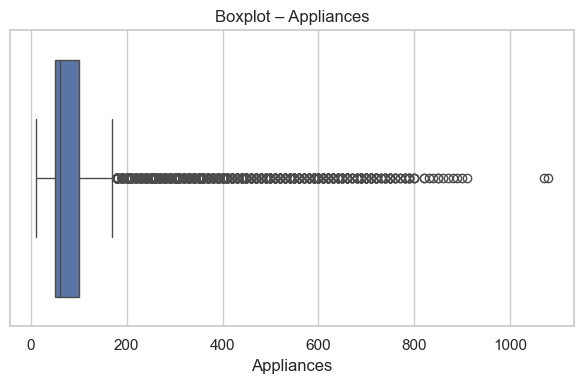
\includegraphics[width=\textwidth,height=0.68\textheight,keepaspectratio]{figures/PL01.png}
\caption[Boxplot của biến Appliances và ngưỡng IQR (Notebook cell 18).]{Boxplot của biến Appliances và ngưỡng IQR (nguồn: Notebook ABC(3), cell 18).}\label{fig:pl1}
\end{figure}

\emph{Outlier Analysis; 2.138 quan sát được gắn cờ, không bị xóa.}

\begin{figure}[H]
\centering
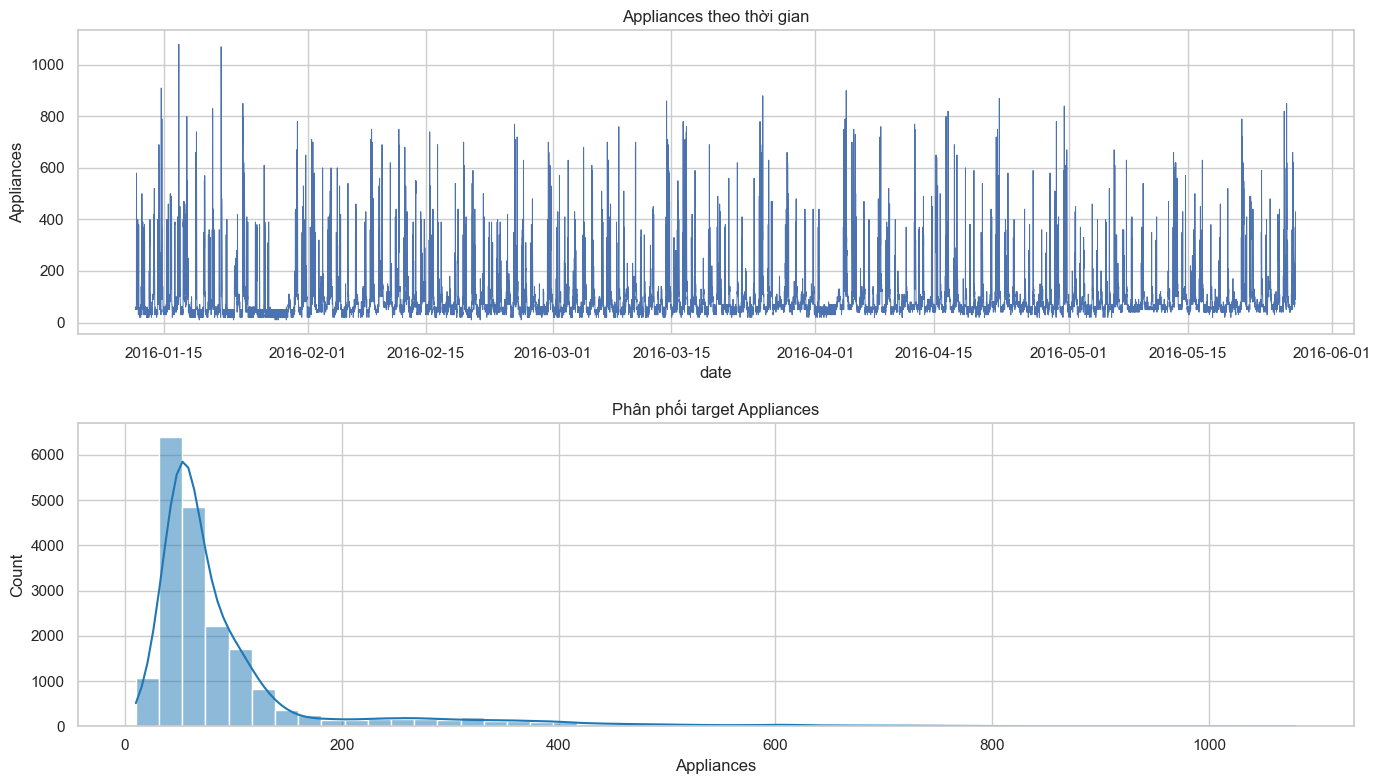
\includegraphics[width=\textwidth,height=0.68\textheight,keepaspectratio]{figures/PL02.png}
\caption[Chuỗi thời gian và phân phối của Appliances (Notebook cell 40).]{Chuỗi thời gian và phân phối của Appliances (nguồn: Notebook ABC(3), cell 40).}\label{fig:pl2}
\end{figure}

\emph{Biểu đồ mục tiêu và histogram; dữ liệu KAG.}

\begin{figure}[H]
\centering
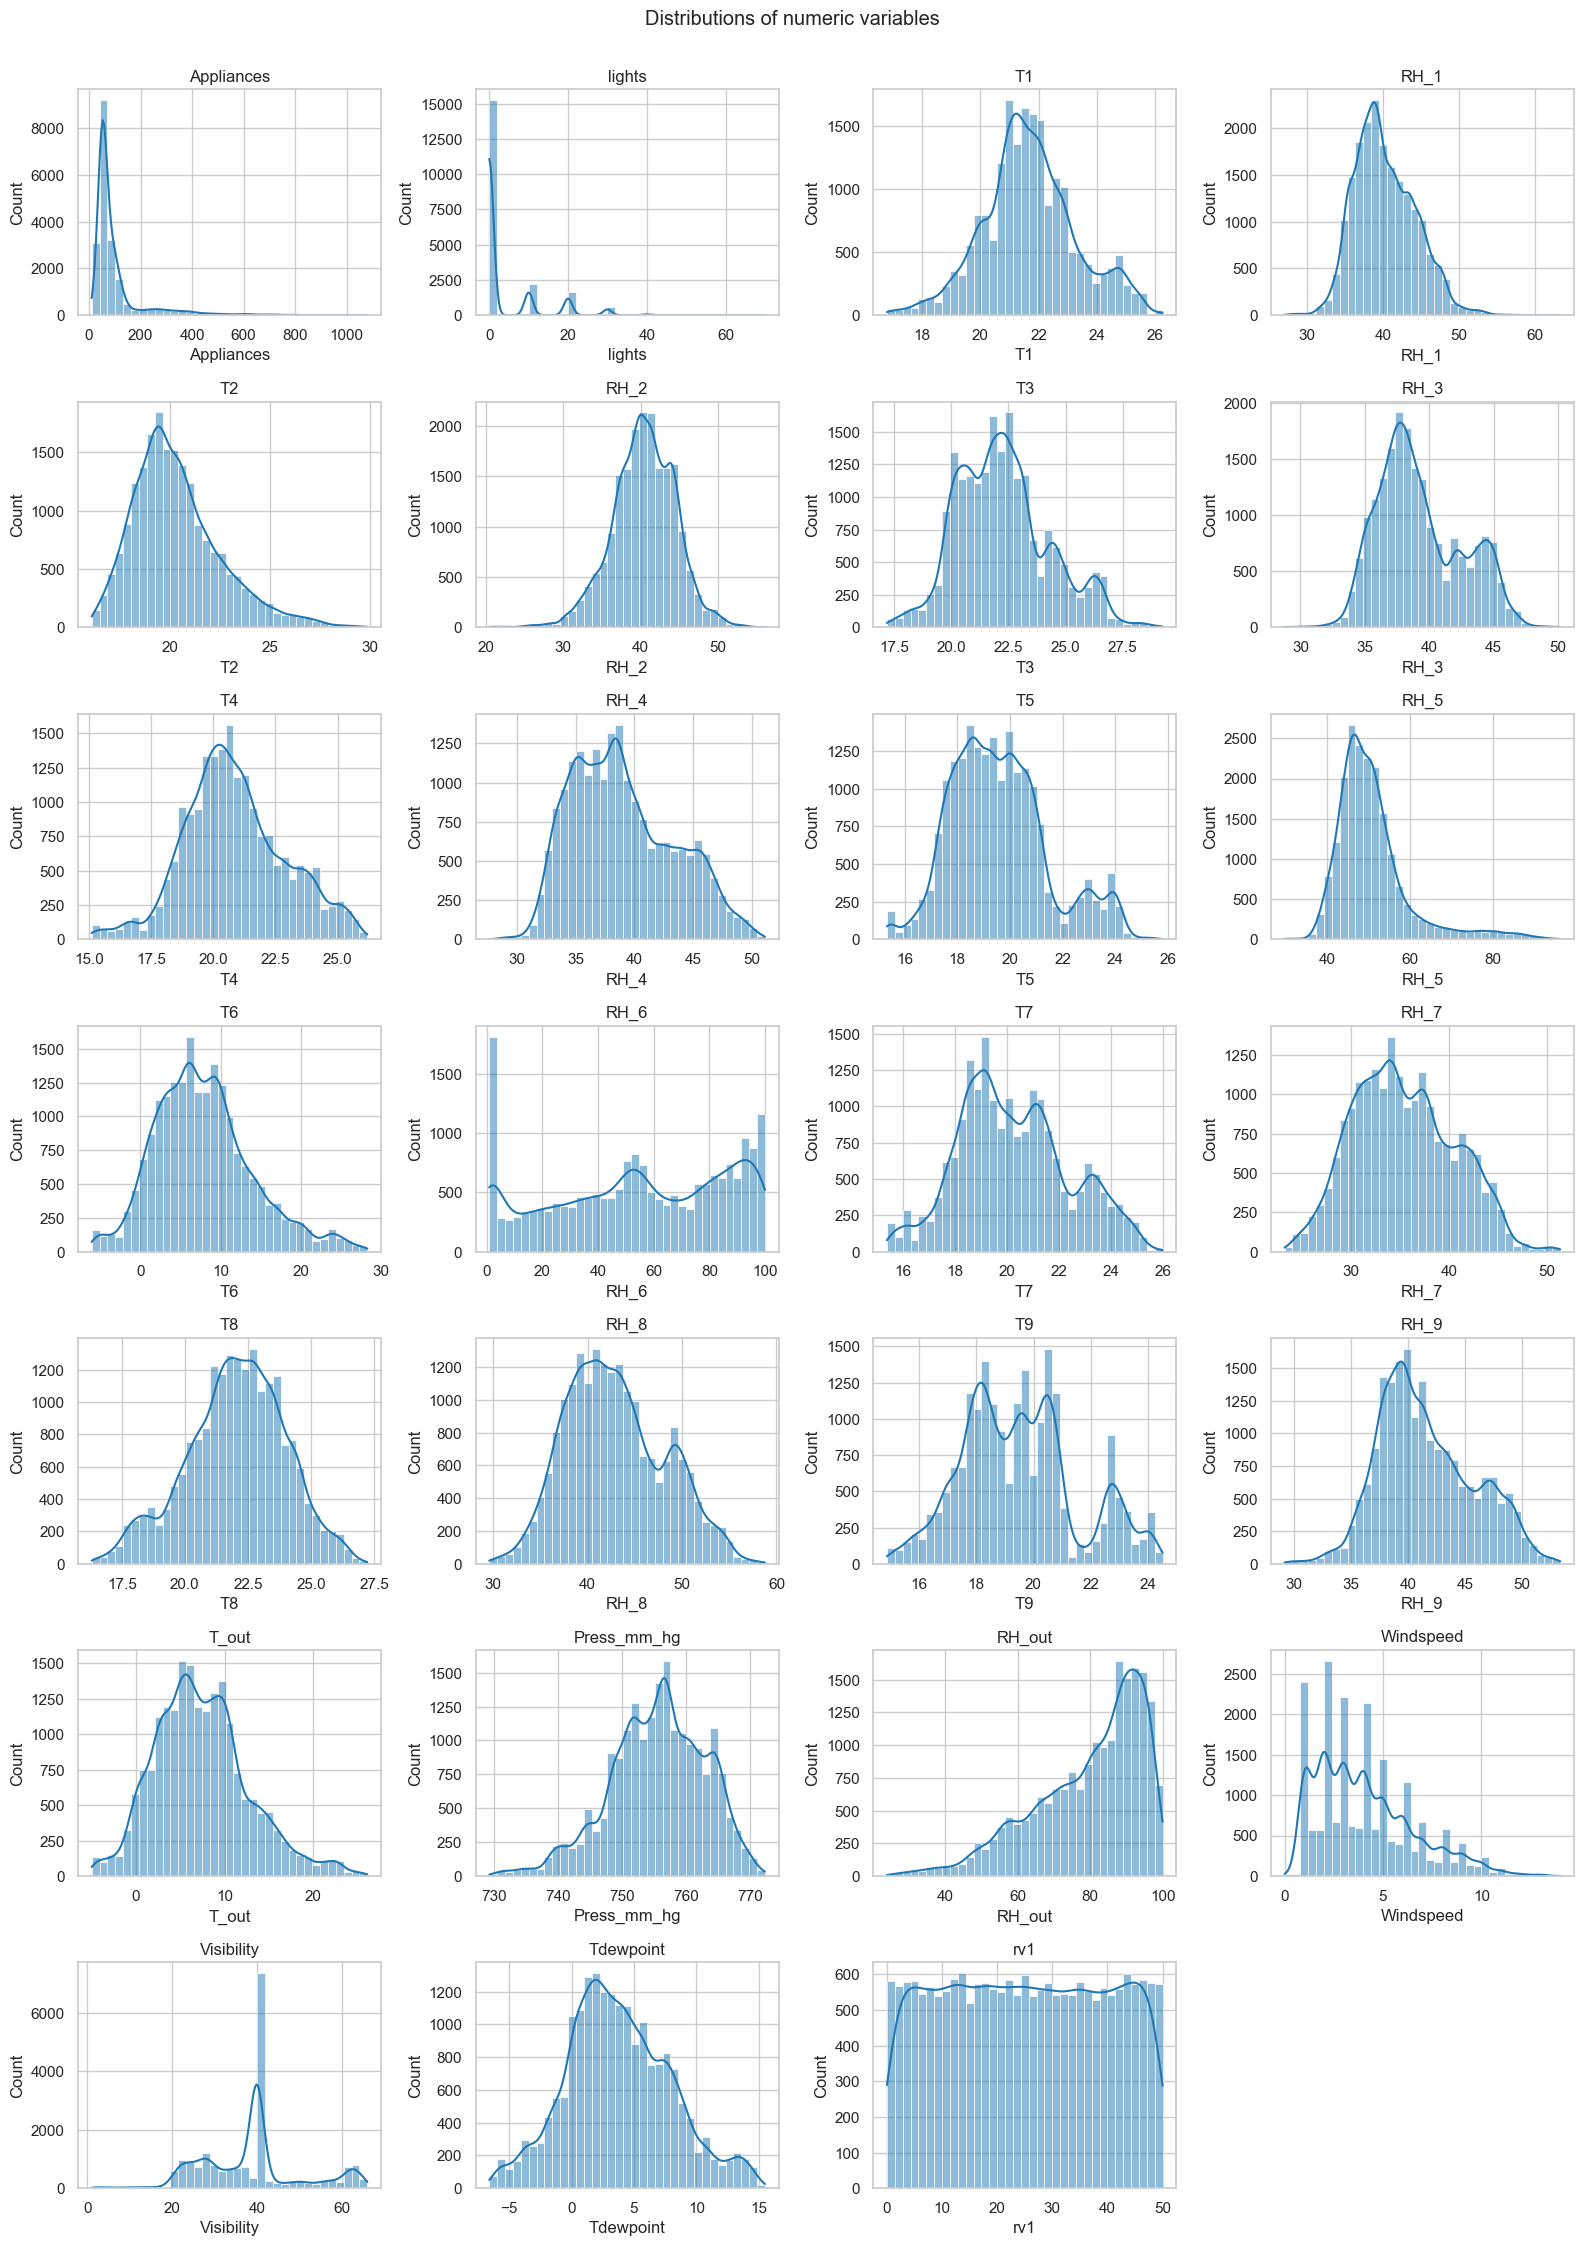
\includegraphics[width=\textwidth,height=0.68\textheight,keepaspectratio]{figures/PL03.png}
\caption[Phân phối các biến số trong dataset (Notebook cell 40).]{Phân phối các biến số trong dataset (nguồn: Notebook ABC(3), cell 40).}\label{fig:pl3}
\end{figure}

\emph{Các histogram của biến số sau làm sạch cột trùng.}

\begin{figure}[H]
\centering
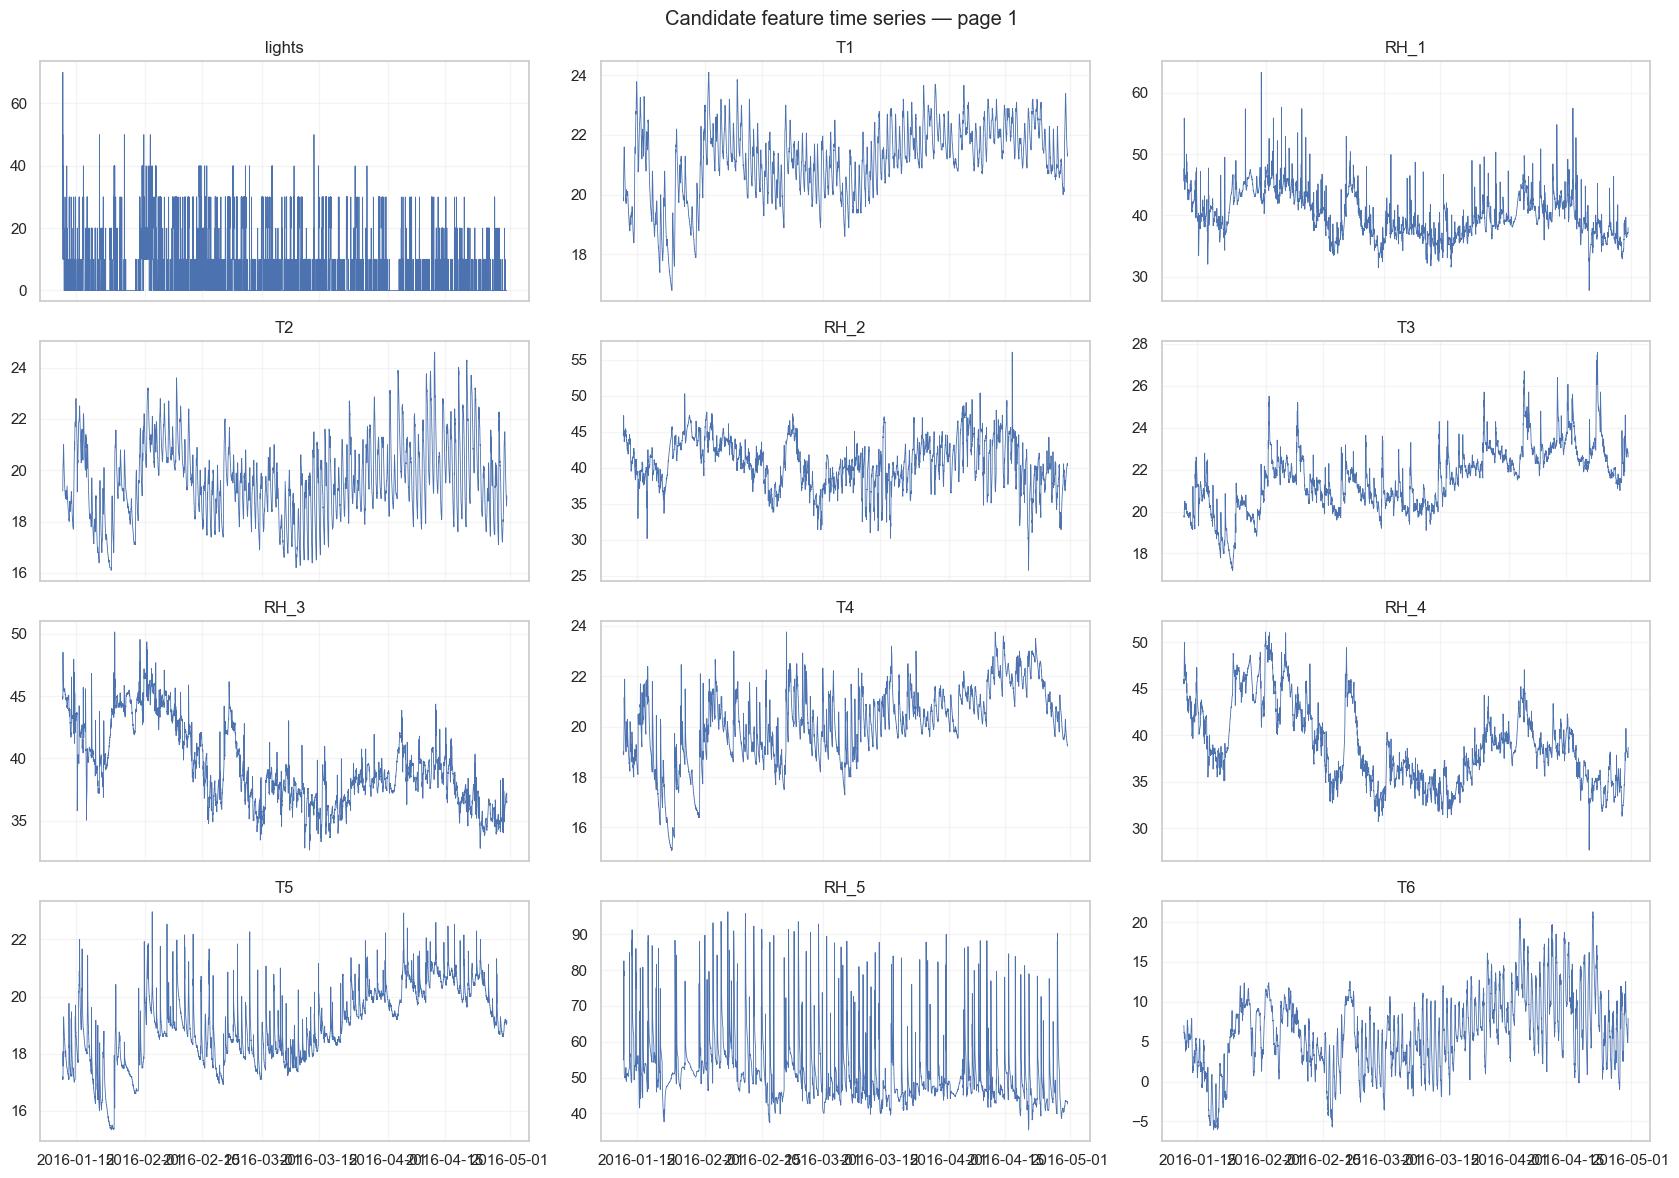
\includegraphics[width=\textwidth,height=0.68\textheight,keepaspectratio]{figures/PL04.png}
\caption[Diễn biến theo thời gian của nhóm đặc trưng - trang 1 (Notebook cell 42).]{Diễn biến theo thời gian của nhóm đặc trưng - trang 1 (nguồn: Notebook ABC(3), cell 42).}\label{fig:pl4}
\end{figure}

\emph{Candidate features; plot tuần tự.}

\begin{figure}[H]
\centering
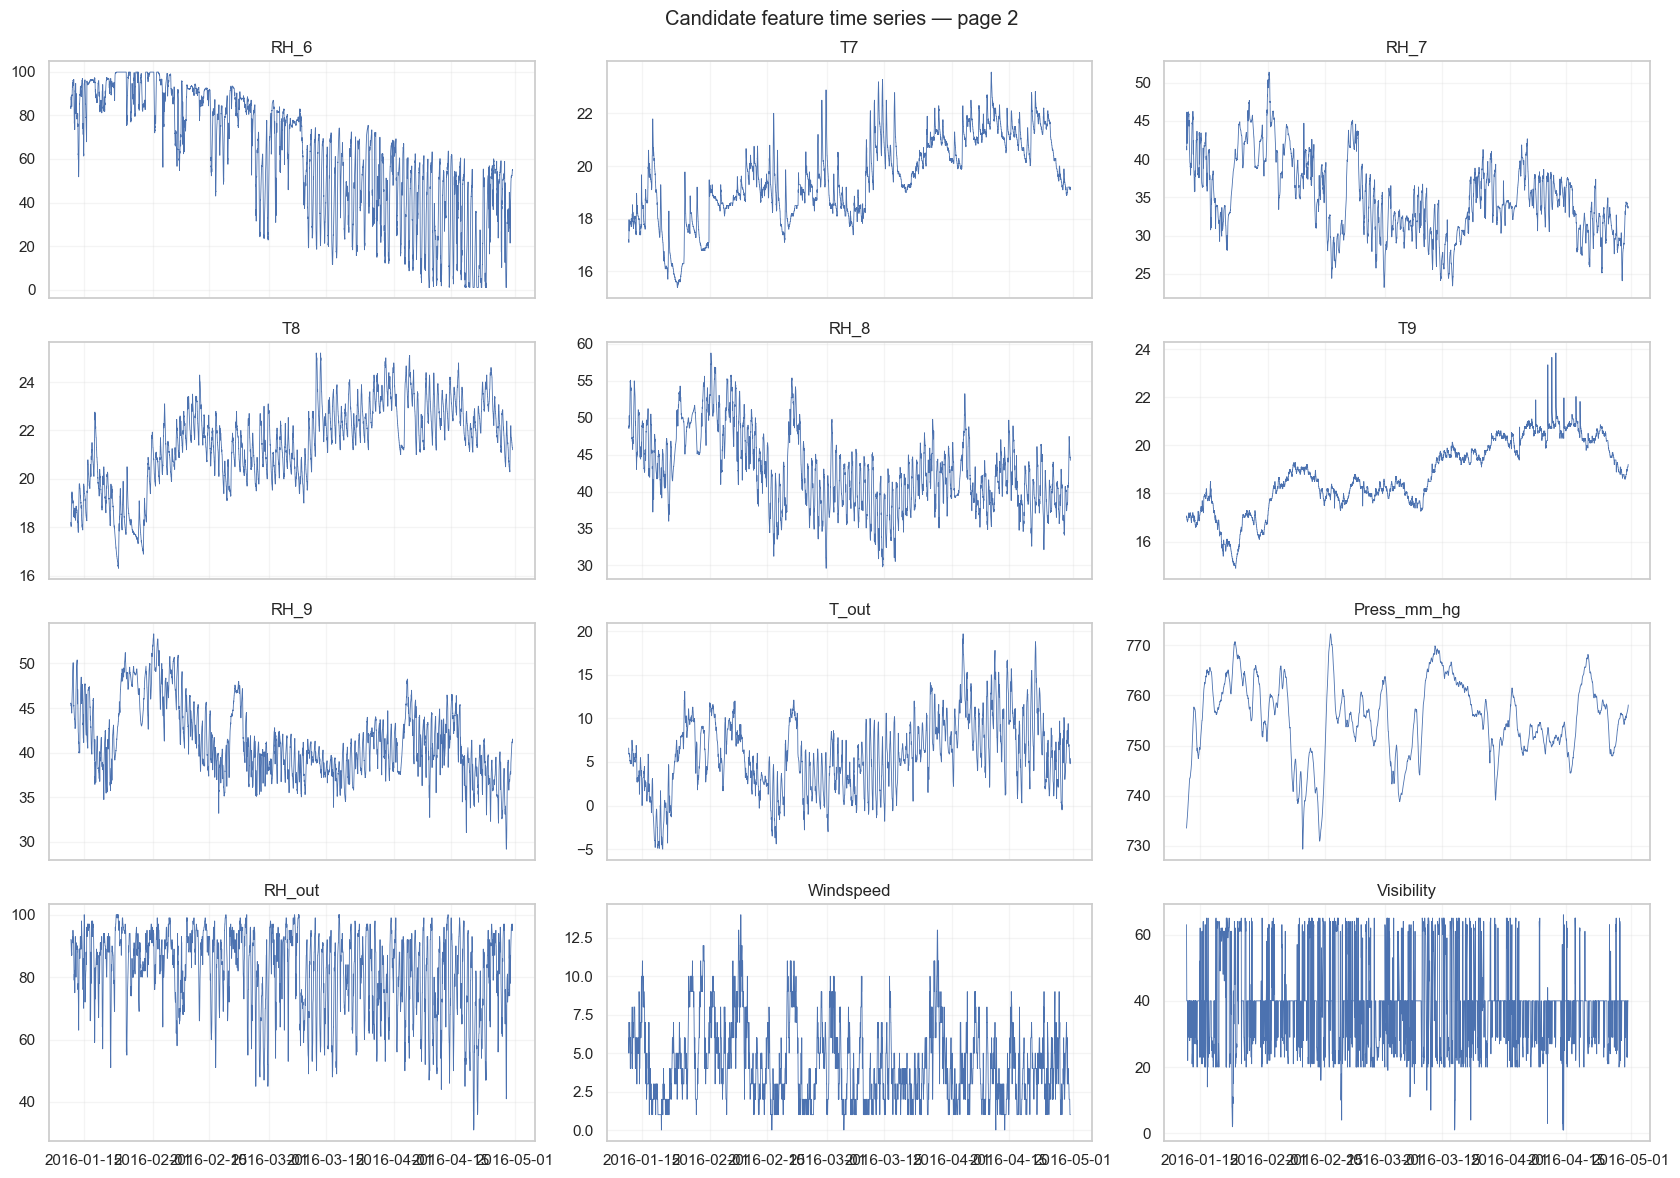
\includegraphics[width=\textwidth,height=0.68\textheight,keepaspectratio]{figures/PL05.png}
\caption[Diễn biến theo thời gian của nhóm đặc trưng - trang 2 (Notebook cell 42).]{Diễn biến theo thời gian của nhóm đặc trưng - trang 2 (nguồn: Notebook ABC(3), cell 42).}\label{fig:pl5}
\end{figure}

\emph{Candidate features; plot tuần tự.}

\begin{figure}[H]
\centering
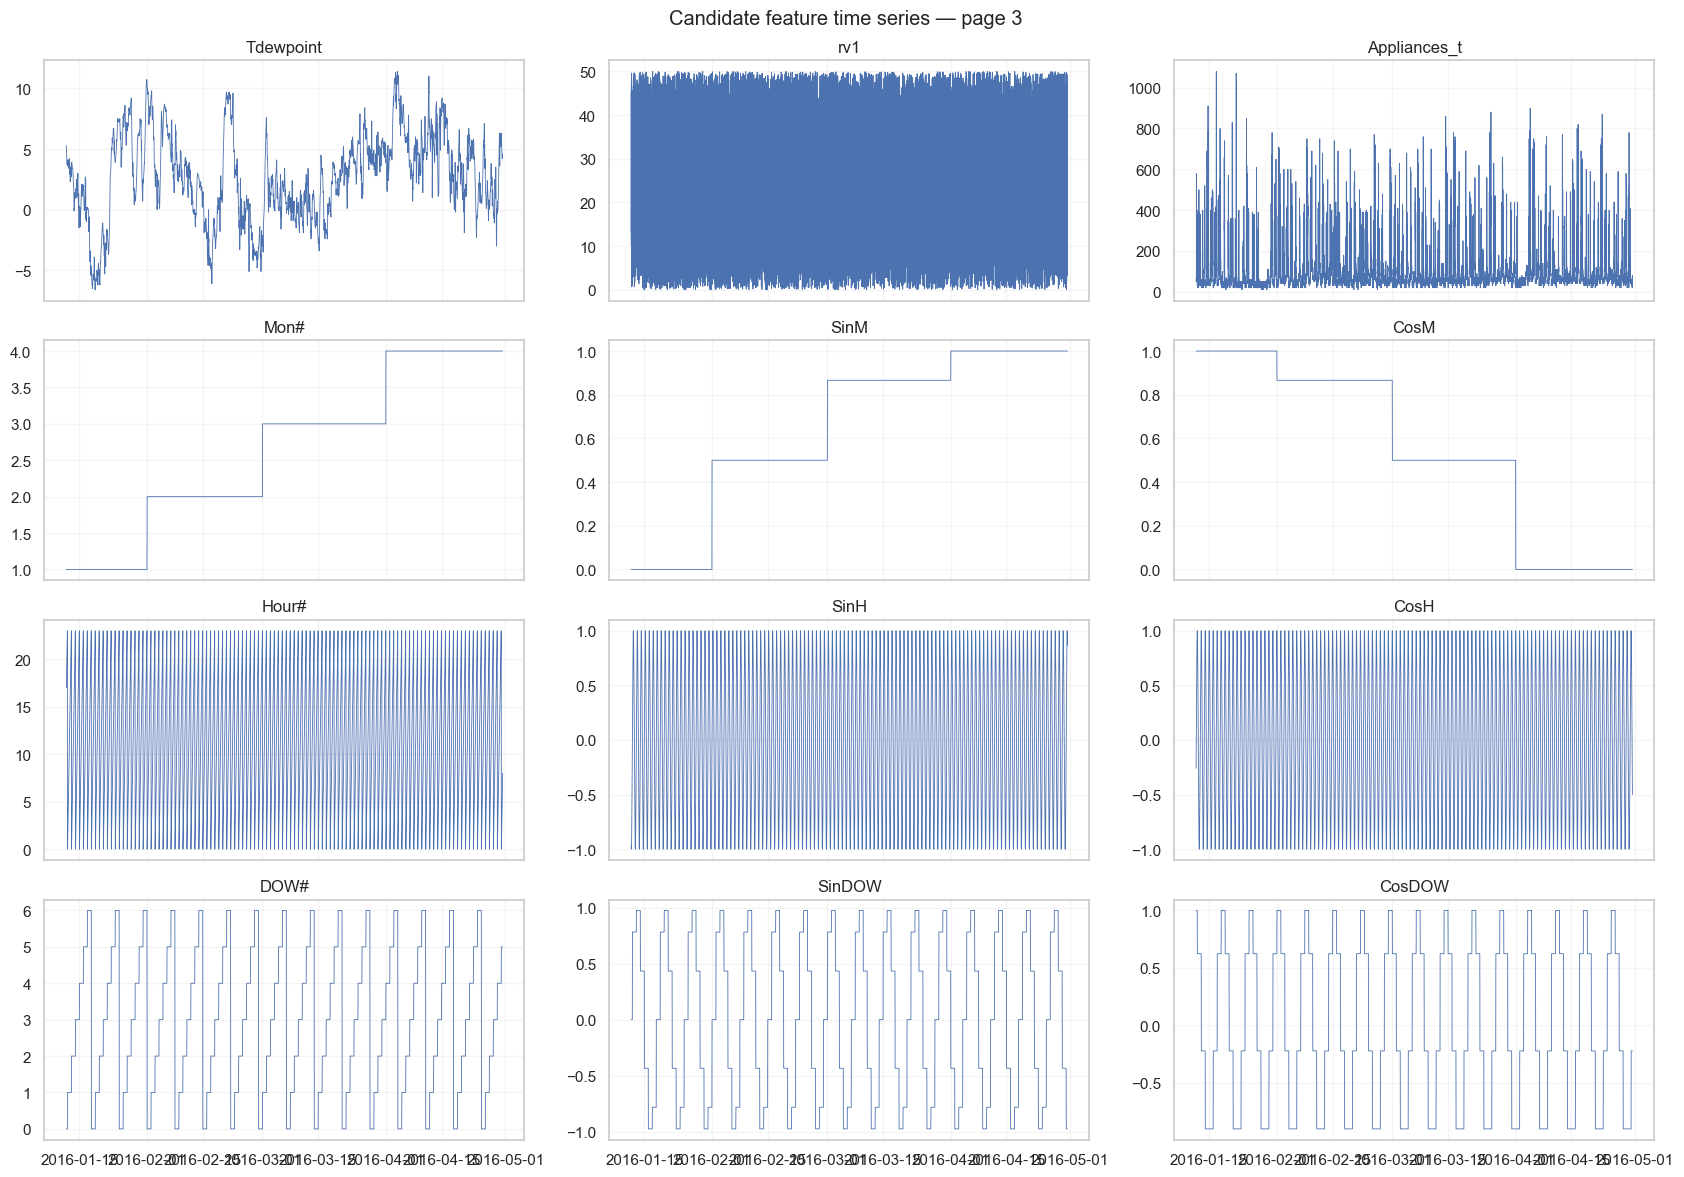
\includegraphics[width=\textwidth,height=0.68\textheight,keepaspectratio]{figures/PL06.png}
\caption[Diễn biến theo thời gian của nhóm đặc trưng - trang 3 (Notebook cell 42).]{Diễn biến theo thời gian của nhóm đặc trưng - trang 3 (nguồn: Notebook ABC(3), cell 42).}\label{fig:pl6}
\end{figure}

\emph{Candidate features; plot tuần tự.}

\begin{figure}[H]
\centering
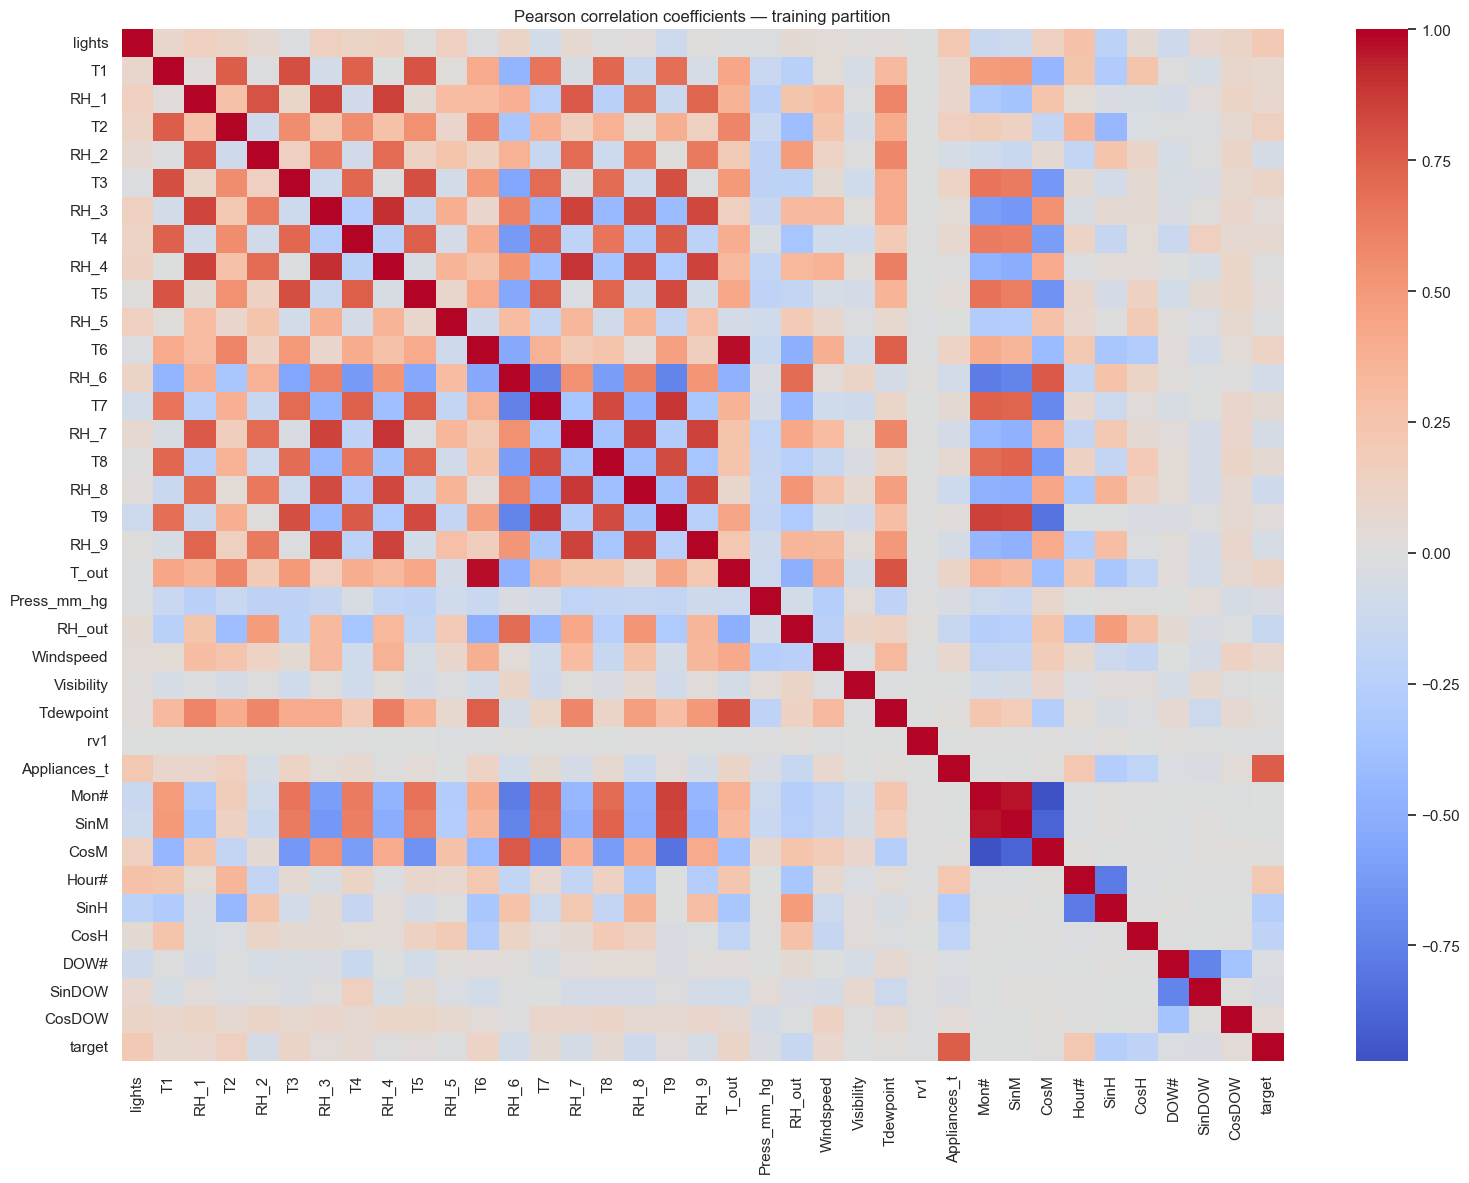
\includegraphics[width=\textwidth,height=0.68\textheight,keepaspectratio]{figures/PL07.png}
\caption[Heatmap Pearson correlation trên training partition (Notebook cell 44).]{Heatmap Pearson correlation trên training partition (nguồn: Notebook ABC(3), cell 44).}\label{fig:pl7}
\end{figure}

\emph{Correlation matrix; calculated from training data.}

\begin{figure}[H]
\centering
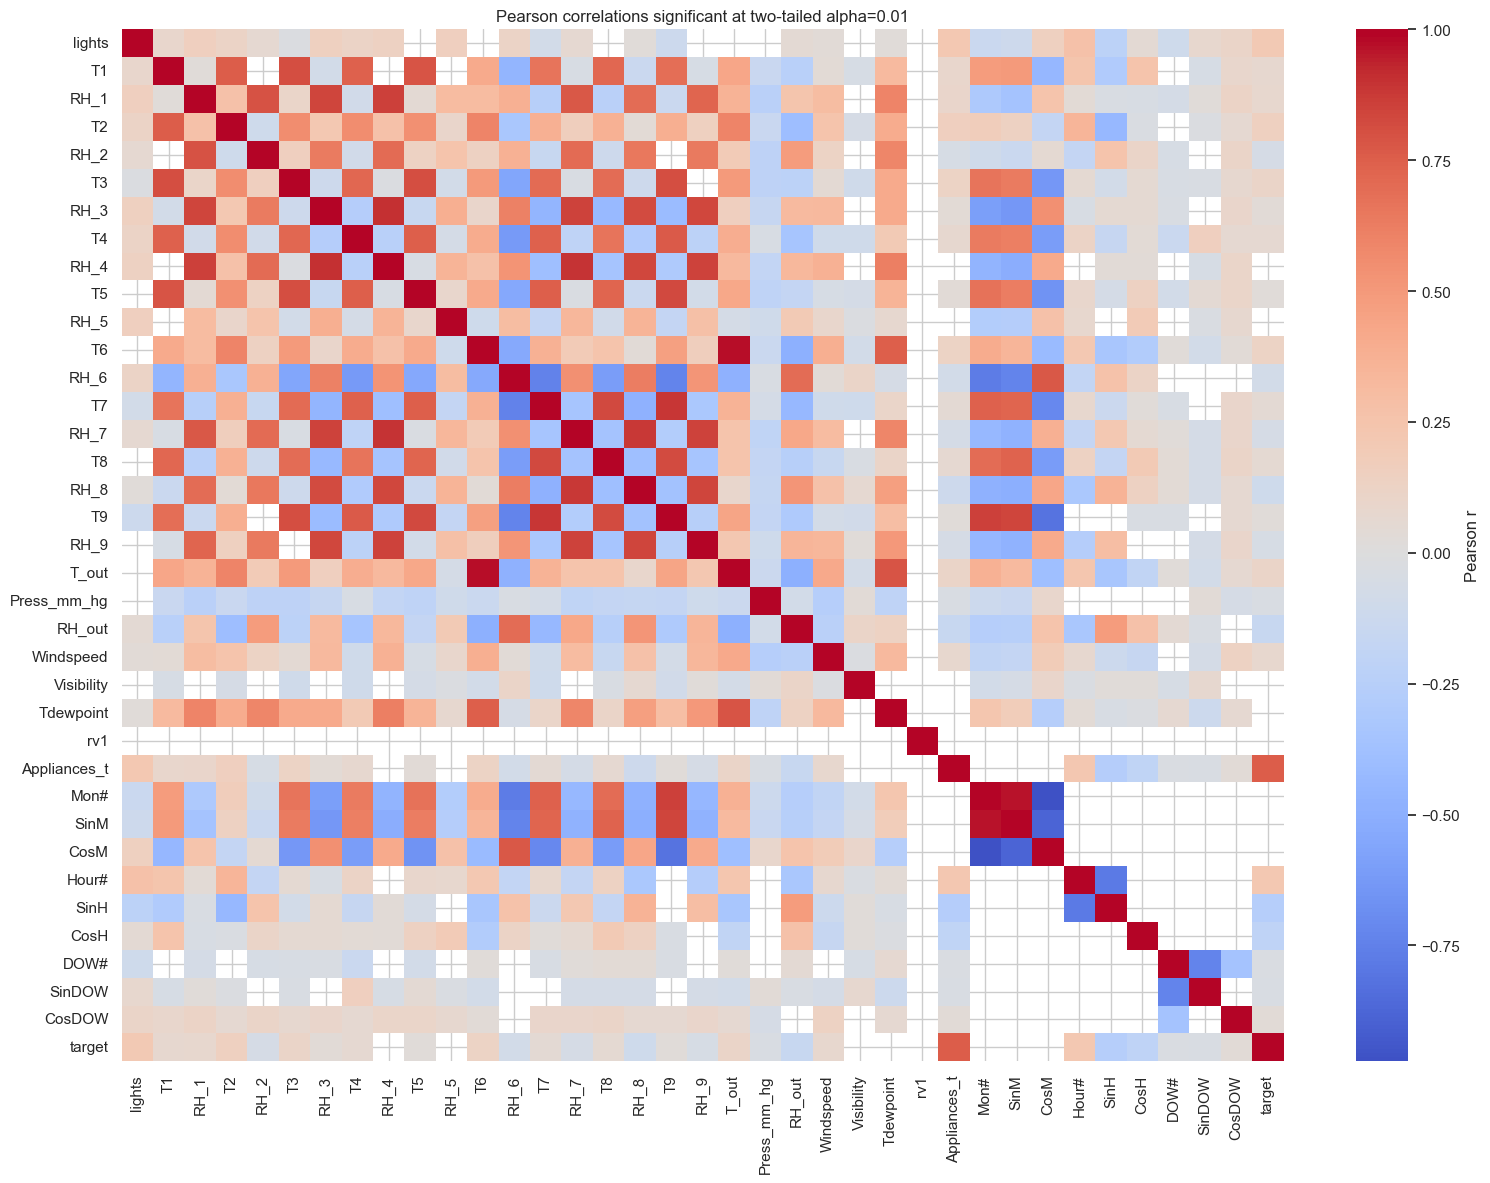
\includegraphics[width=\textwidth,height=0.68\textheight,keepaspectratio]{figures/PL08.png}
\caption[Heatmap Pearson chỉ giữ các cặp có ý nghĩa danh nghĩa (Notebook cell 44).]{Heatmap Pearson chỉ giữ các cặp có ý nghĩa danh nghĩa (nguồn: Notebook ABC(3), cell 44).}\label{fig:pl8}
\end{figure}

\emph{Two-tailed Pearson; alpha = 0.01; cần lưu ý tự tương quan thời gian.}

\begin{figure}[H]
\centering
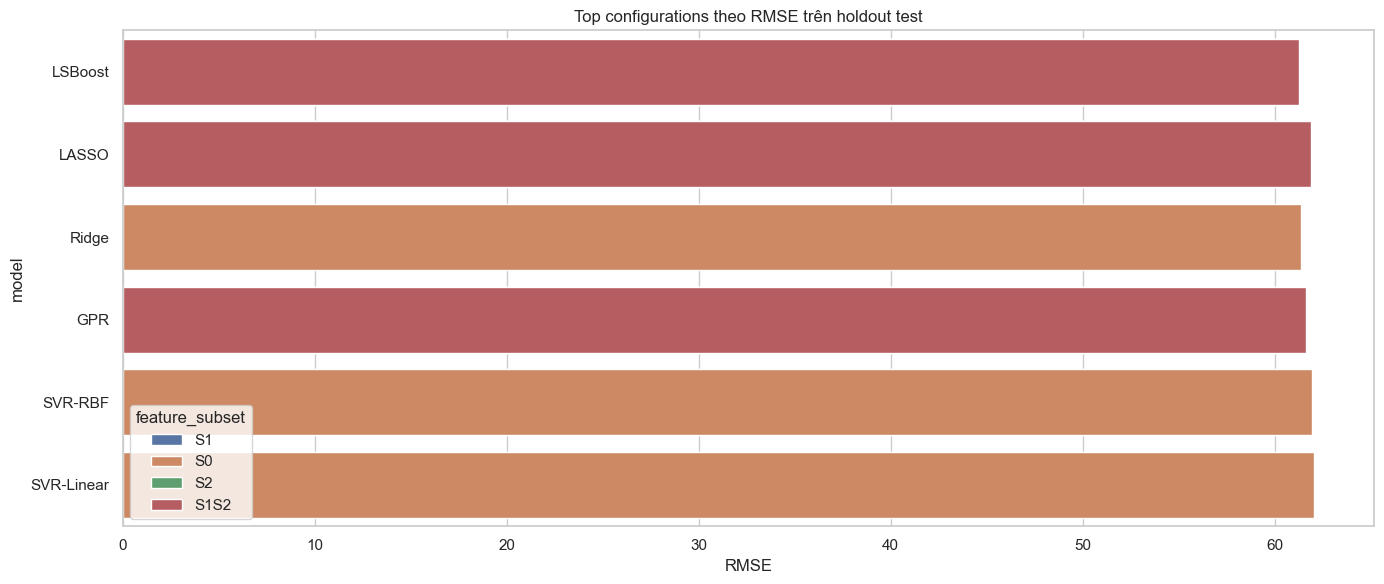
\includegraphics[width=\textwidth,height=0.68\textheight,keepaspectratio]{figures/PL09.png}
\caption[So sánh cấu hình có RMSE thấp trên holdout test (Notebook cell 56).]{So sánh cấu hình có RMSE thấp trên holdout test (nguồn: Notebook ABC(3), cell 56).}\label{fig:pl9}
\end{figure}

\emph{Top configurations; nguồn paper\_results và baseline\_results.}

\begin{figure}[H]
\centering
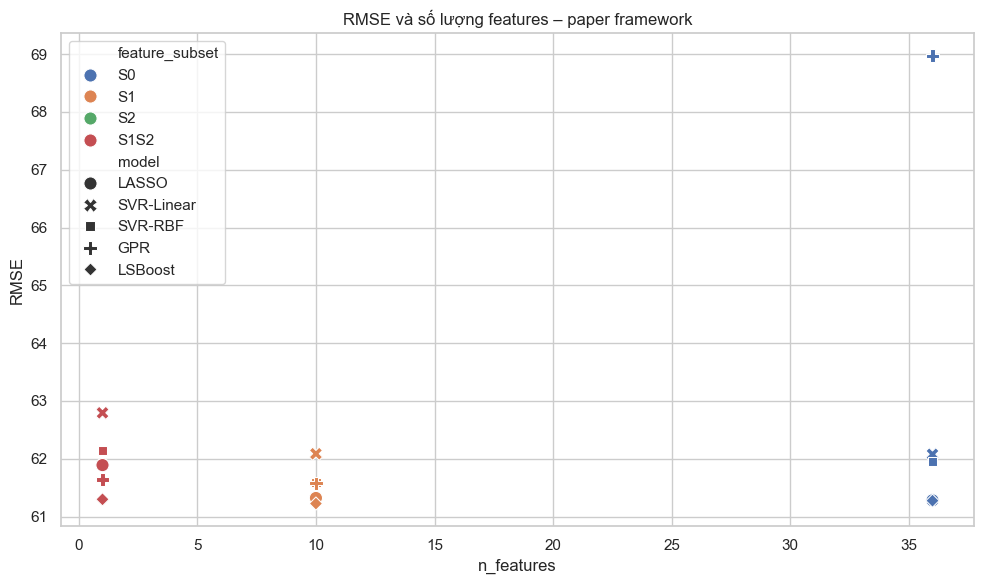
\includegraphics[width=\textwidth,height=0.68\textheight,keepaspectratio]{figures/PL10.png}
\caption[Quan hệ giữa số đặc trưng và RMSE (Notebook cell 56).]{Quan hệ giữa số đặc trưng và RMSE (nguồn: Notebook ABC(3), cell 56).}\label{fig:pl10}
\end{figure}

\emph{Mối quan hệ dimensionality–error trên các cấu hình.}

\begin{figure}[H]
\centering
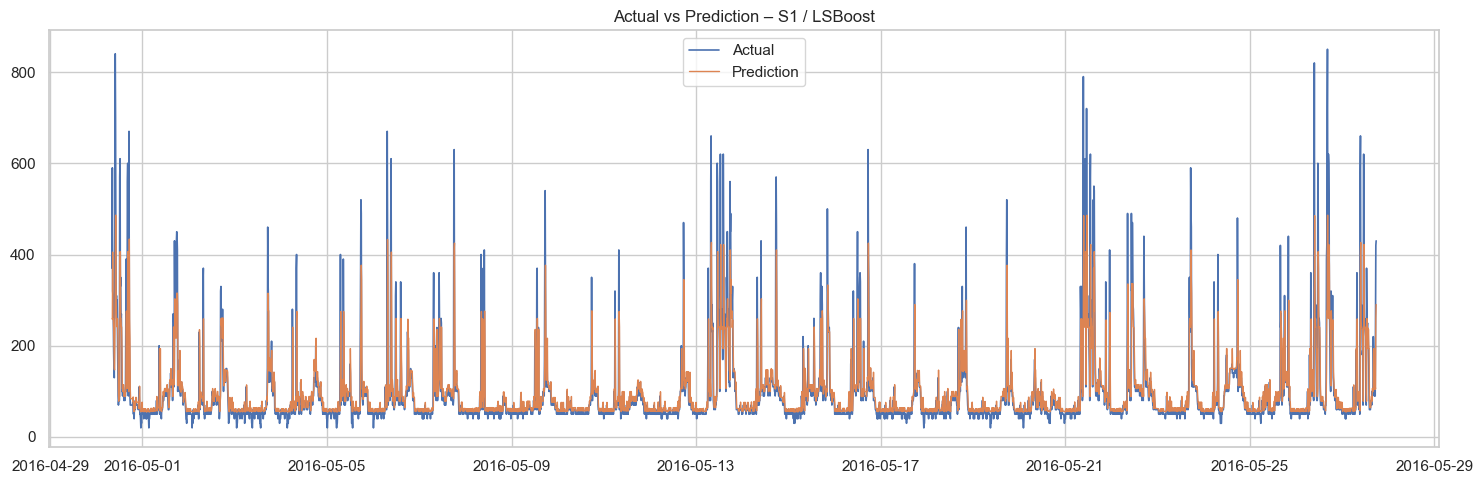
\includegraphics[width=\textwidth,height=0.68\textheight,keepaspectratio]{figures/PL11.png}
\caption[Giá trị thực và dự báo của cấu hình S1–LSBoost (Notebook cell 56).]{Giá trị thực và dự báo của cấu hình S1–LSBoost (nguồn: Notebook ABC(3), cell 56).}\label{fig:pl11}
\end{figure}

\emph{Dự báo trên holdout test.}

\begin{figure}[H]
\centering
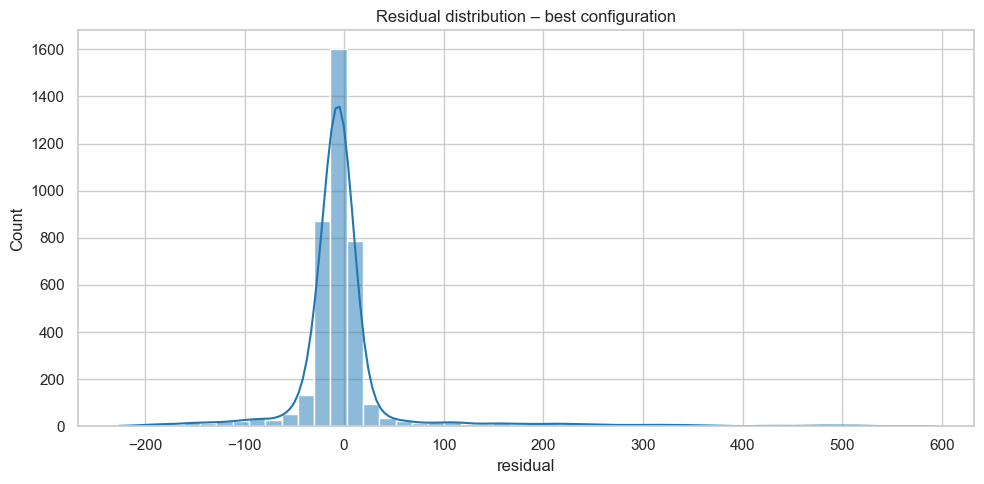
\includegraphics[width=\textwidth,height=0.68\textheight,keepaspectratio]{figures/PL12.png}
\caption[Phân phối residual của cấu hình tốt nhất (Notebook cell 56).]{Phân phối residual của cấu hình tốt nhất (nguồn: Notebook ABC(3), cell 56).}\label{fig:pl12}
\end{figure}

\emph{Residual distribution trên holdout test.}

\begin{figure}[H]
\centering
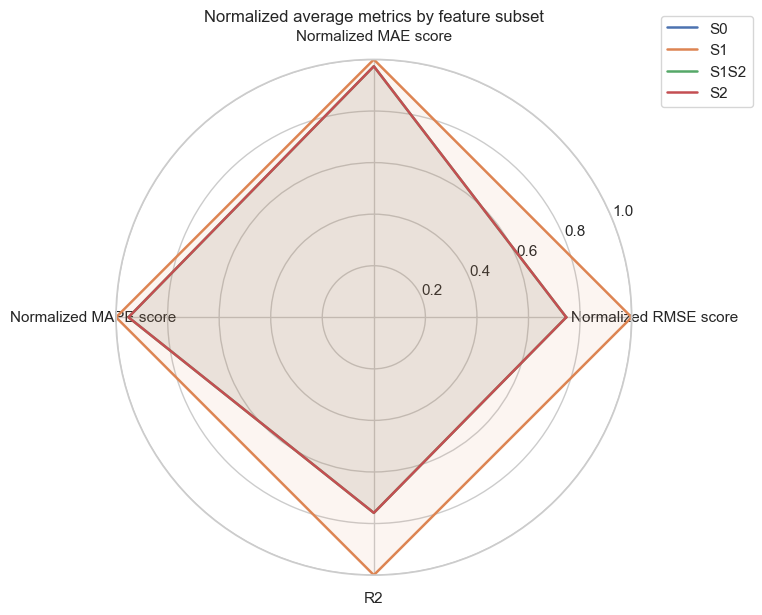
\includegraphics[width=\textwidth,height=0.68\textheight,keepaspectratio]{figures/PL13.png}
\caption[Radar chart hiệu năng chuẩn hóa theo feature subset (Notebook cell 56).]{Radar chart hiệu năng chuẩn hóa theo feature subset (nguồn: Notebook ABC(3), cell 56).}\label{fig:pl13}
\end{figure}

\emph{Chỉ số đã chuẩn hóa phục vụ trực quan hóa; tham chiếu bảng metric gốc.}

\begin{figure}[H]
\centering
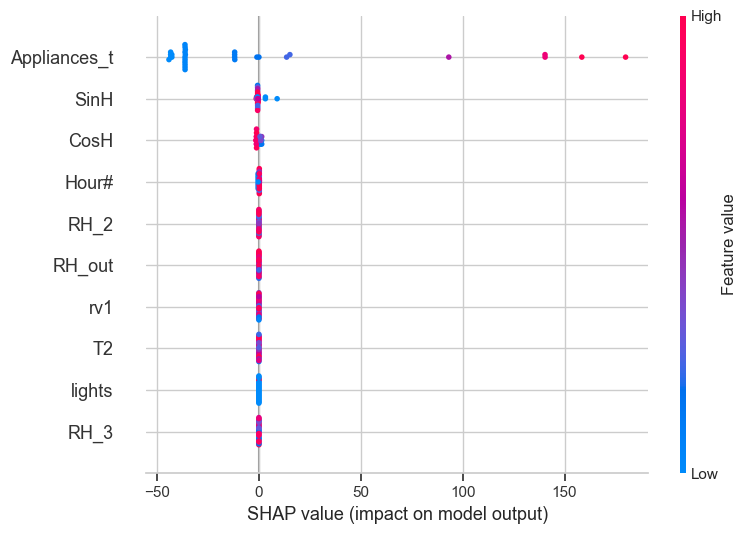
\includegraphics[width=\textwidth,height=0.68\textheight,keepaspectratio]{figures/PL14.png}
\caption[SHAP summary cho S1–LSBoost (Notebook cell 58).]{SHAP summary cho S1–LSBoost (nguồn: Notebook ABC(3), cell 58).}\label{fig:pl14}
\end{figure}

\emph{Permutation\allowbreak Explainer; 10 features, max\_evals=21.}

\begin{figure}[H]
\centering
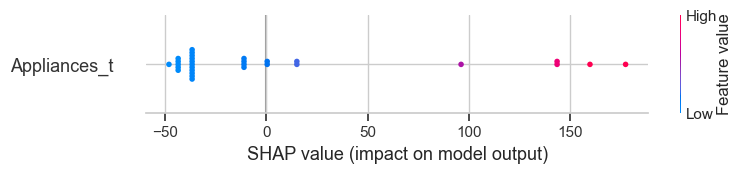
\includegraphics[width=\textwidth,height=0.68\textheight,keepaspectratio]{figures/PL15.png}
\caption[SHAP summary cho S2–LSBoost (Notebook cell 58).]{SHAP summary cho S2–LSBoost (nguồn: Notebook ABC(3), cell 58).}\label{fig:pl15}
\end{figure}

\emph{Permutation\allowbreak Explainer; 1 feature, max\_evals=3.}

\begin{figure}[H]
\centering
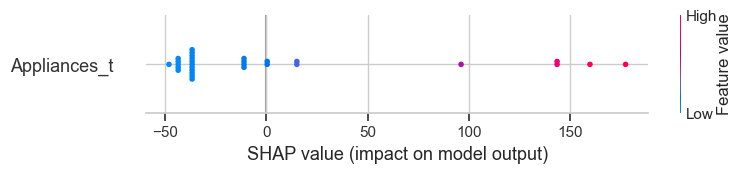
\includegraphics[width=\textwidth,height=0.68\textheight,keepaspectratio]{figures/PL16.png}
\caption[SHAP summary cho S1S2–LSBoost (Notebook cell 58).]{SHAP summary cho S1S2–LSBoost (nguồn: Notebook ABC(3), cell 58).}\label{fig:pl16}
\end{figure}

\emph{Permutation\allowbreak Explainer; 1 feature, max\_evals=3.}

\begin{figure}[H]
\centering
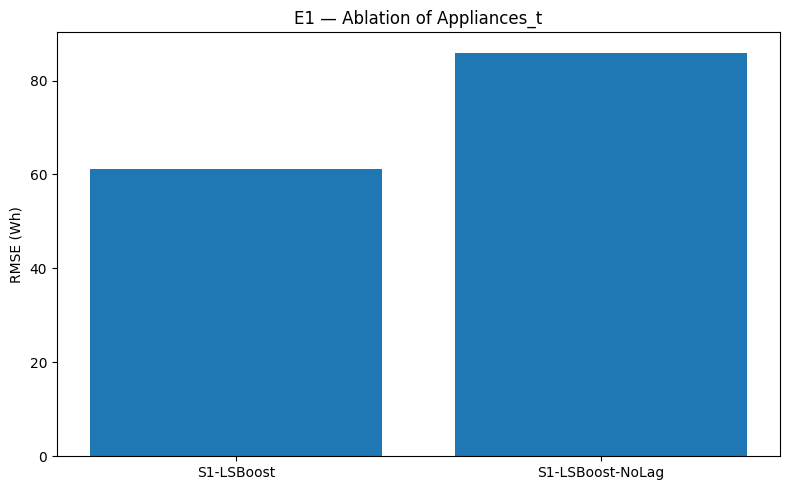
\includegraphics[width=\textwidth,height=0.68\textheight,keepaspectratio]{figures/PL17.png}
\caption[E1: so sánh RMSE khi loại Appliances\_t khỏi S1 (Notebook cell 64).]{E1: so sánh RMSE khi loại Appliances\_t khỏi S1 (nguồn: Notebook ABC(3), cell 64).}\label{fig:pl17}
\end{figure}

\emph{Lag Feature Ablation có kiểm soát; 10 versus 9 features.}

\begin{figure}[H]
\centering
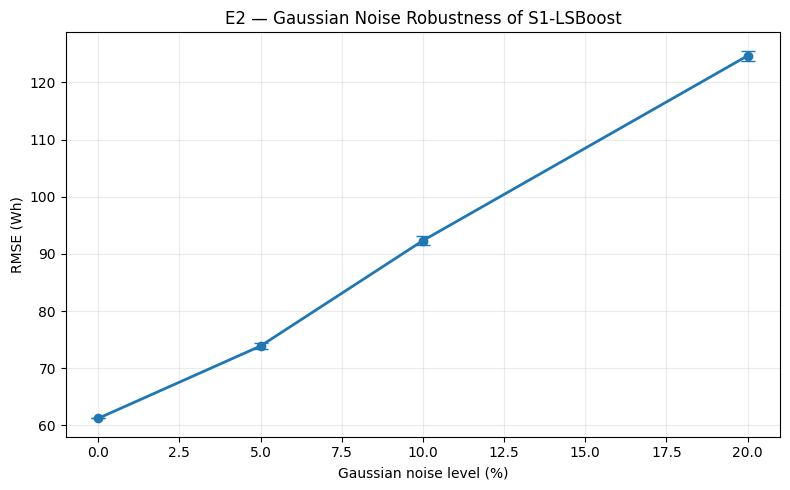
\includegraphics[width=\textwidth,height=0.68\textheight,keepaspectratio]{figures/PL18.png}
\caption[E2: độ nhạy RMSE trước nhiễu Gaussian (Notebook cell 65).]{E2: độ nhạy RMSE trước nhiễu Gaussian (nguồn: Notebook ABC(3), cell 65).}\label{fig:pl18}
\end{figure}

\emph{4 mức noise; 5 lần lặp mỗi mức.}

\chapter{Bảng kết quả thực nghiệm}\label{app:results}
\setcounter{table}{0}\renewcommand{\thetable}{PL.B.\arabic{table}}

\section{Toàn bộ 20 cấu hình forecasting}\label{b.1.-touxe0n-bux1ed9-20-cux1ea5u-huxecnh-forecasting}

\begin{longtable}[]{@{}
  >{\raggedright\arraybackslash}p{(\columnwidth - 12\tabcolsep) * \real{0.1429}}
  >{\raggedright\arraybackslash}p{(\columnwidth - 12\tabcolsep) * \real{0.1429}}
  >{\raggedright\arraybackslash}p{(\columnwidth - 12\tabcolsep) * \real{0.1429}}
  >{\raggedright\arraybackslash}p{(\columnwidth - 12\tabcolsep) * \real{0.1429}}
  >{\raggedright\arraybackslash}p{(\columnwidth - 12\tabcolsep) * \real{0.1429}}
  >{\raggedright\arraybackslash}p{(\columnwidth - 12\tabcolsep) * \real{0.1429}}
  >{\raggedright\arraybackslash}p{(\columnwidth - 12\tabcolsep) * \real{0.1429}}@{}}
\caption{Toàn bộ 20 cấu hình forecasting.}\label{tab:app-b-0-to-n-b-20-c-u-h-nh-forecasting}\\
\toprule\noalign{}
\toprule\noalign{}
\begin{minipage}[b]{\linewidth}\raggedright
\textbf{Subset}
\end{minipage} & \begin{minipage}[b]{\linewidth}\raggedright
\textbf{Model}
\end{minipage} & \begin{minipage}[b]{\linewidth}\raggedright
\textbf{n}
\end{minipage} & \begin{minipage}[b]{\linewidth}\raggedright
\textbf{RMSE}
\end{minipage} & \begin{minipage}[b]{\linewidth}\raggedright
\textbf{MAE}
\end{minipage} & \begin{minipage}[b]{\linewidth}\raggedright
\textbf{MAPE \%}
\end{minipage} & \begin{minipage}[b]{\linewidth}\raggedright
\textbf{R²}
\end{minipage} \\
\midrule\noalign{}
\endfirsthead
\toprule\noalign{}
\begin{minipage}[b]{\linewidth}\raggedright
\textbf{Subset}
\end{minipage} & \begin{minipage}[b]{\linewidth}\raggedright
\textbf{Model}
\end{minipage} & \begin{minipage}[b]{\linewidth}\raggedright
\textbf{n}
\end{minipage} & \begin{minipage}[b]{\linewidth}\raggedright
\textbf{RMSE}
\end{minipage} & \begin{minipage}[b]{\linewidth}\raggedright
\textbf{MAE}
\end{minipage} & \begin{minipage}[b]{\linewidth}\raggedright
\textbf{MAPE \%}
\end{minipage} & \begin{minipage}[b]{\linewidth}\raggedright
\textbf{R²}
\end{minipage} \\
\midrule\noalign{}
\endhead
\bottomrule\noalign{}
\endlastfoot
S1 & LSBoost & 10 & 61.223997 & 26.543855 & 24.2492 & 0.547735 \\
S0 & LSBoost & 36 & 61.274424 & 26.524782 & 24.2216 & 0.546990 \\
S0 & LASSO & 36 & 61.280461 & 27.384938 & 25.8779 & 0.546901 \\
S2 & LSBoost & 1 & 61.297607 & 26.693146 & 24.5056 & 0.546647 \\
S1S2 & LSBoost & 1 & 61.297607 & 26.693146 & 24.5056 & 0.546647 \\
S1 & LASSO & 10 & 61.320689 & 26.929178 & 24.9662 & 0.546305 \\
S1 & GPR & 10 & 61.575189 & 27.337066 & 25.2211 & 0.542532 \\
S1 & SVR-RBF & 10 & 61.587307 & 25.240089 & 21.4945 & 0.542352 \\
S1S2 & GPR & 1 & 61.642860 & 26.880983 & 25.4322 & 0.541526 \\
S2 & GPR & 1 & 61.642860 & 26.880983 & 25.4322 & 0.541526 \\
S1S2 & LASSO & 1 & 61.889770 & 27.284338 & 26.0961 & 0.537845 \\
S2 & LASSO & 1 & 61.889770 & 27.284338 & 26.0961 & 0.537845 \\
S0 & SVR-RBF & 36 & 61.957310 & 25.266593 & 20.8677 & 0.536836 \\
S0 & SVR-Linear & 36 & 62.076702 & 25.223017 & 21.2298 & 0.535049 \\
S1 & SVR-Linear & 10 & 62.086319 & 25.074346 & 20.9799 & 0.534905 \\
S2 & SVR-RBF & 1 & 62.138361 & 25.436815 & 21.4556 & 0.534125 \\
S1S2 & SVR-RBF & 1 & 62.138361 & 25.436815 & 21.4556 & 0.534125 \\
S2 & SVR-Linear & 1 & 62.793984 & 25.196022 & 20.4339 & 0.524243 \\
S1S2 & SVR-Linear & 1 & 62.793984 & 25.196022 & 20.4339 & 0.524243 \\
S0 & GPR & 36 & 68.969188 & 40.661501 & 45.7191 & 0.426069 \\
\end{longtable}

\section{Baseline results}\label{b.2.-baseline-results}

\begin{longtable}[]{@{}
  >{\raggedright\arraybackslash}p{(\columnwidth - 10\tabcolsep) * \real{0.1667}}
  >{\raggedright\arraybackslash}p{(\columnwidth - 10\tabcolsep) * \real{0.1667}}
  >{\raggedright\arraybackslash}p{(\columnwidth - 10\tabcolsep) * \real{0.1667}}
  >{\raggedright\arraybackslash}p{(\columnwidth - 10\tabcolsep) * \real{0.1667}}
  >{\raggedright\arraybackslash}p{(\columnwidth - 10\tabcolsep) * \real{0.1667}}
  >{\raggedright\arraybackslash}p{(\columnwidth - 10\tabcolsep) * \real{0.1667}}@{}}
\caption{Baseline results.}\label{tab:app-b-1-baseline-results}\\
\toprule\noalign{}
\toprule\noalign{}
\begin{minipage}[b]{\linewidth}\raggedright
\textbf{Baseline}
\end{minipage} & \begin{minipage}[b]{\linewidth}\raggedright
\textbf{n features}
\end{minipage} & \begin{minipage}[b]{\linewidth}\raggedright
\textbf{RMSE}
\end{minipage} & \begin{minipage}[b]{\linewidth}\raggedright
\textbf{MAE}
\end{minipage} & \begin{minipage}[b]{\linewidth}\raggedright
\textbf{MAPE \%}
\end{minipage} & \begin{minipage}[b]{\linewidth}\raggedright
\textbf{R²}
\end{minipage} \\
\midrule\noalign{}
\endfirsthead
\toprule\noalign{}
\begin{minipage}[b]{\linewidth}\raggedright
\textbf{Baseline}
\end{minipage} & \begin{minipage}[b]{\linewidth}\raggedright
\textbf{n features}
\end{minipage} & \begin{minipage}[b]{\linewidth}\raggedright
\textbf{RMSE}
\end{minipage} & \begin{minipage}[b]{\linewidth}\raggedright
\textbf{MAE}
\end{minipage} & \begin{minipage}[b]{\linewidth}\raggedright
\textbf{MAPE \%}
\end{minipage} & \begin{minipage}[b]{\linewidth}\raggedright
\textbf{R²}
\end{minipage} \\
\midrule\noalign{}
\endhead
\bottomrule\noalign{}
\endlastfoot
Persistence & 1 & 66.437640 & 26.650621 & 21.9361 & 0.467429 \\
Ridge & 36 & 61.393249 & 26.333199 & 23.1436 & 0.545231 \\
RandomForest & 36 & 97.809147 & 65.064723 & 72.5555 & -0.154273 \\
HistGradient\allowbreak Boosting & 36 & 64.144688 & 33.990690 & 34.2283 & 0.503555 \\
\end{longtable}

\section{SHAP feature importance}\label{b.3.-shap-feature-importance}

\begin{longtable}[]{@{}
  >{\raggedright\arraybackslash}p{(\columnwidth - 10\tabcolsep) * \real{0.1667}}
  >{\raggedright\arraybackslash}p{(\columnwidth - 10\tabcolsep) * \real{0.1667}}
  >{\raggedright\arraybackslash}p{(\columnwidth - 10\tabcolsep) * \real{0.1667}}
  >{\raggedright\arraybackslash}p{(\columnwidth - 10\tabcolsep) * \real{0.1667}}
  >{\raggedright\arraybackslash}p{(\columnwidth - 10\tabcolsep) * \real{0.1667}}
  >{\raggedright\arraybackslash}p{(\columnwidth - 10\tabcolsep) * \real{0.1667}}@{}}
\caption{SHAP feature importance.}\label{tab:app-b-2-shap-feature-importance}\\
\toprule\noalign{}
\toprule\noalign{}
\begin{minipage}[b]{\linewidth}\raggedright
\textbf{Track}
\end{minipage} & \begin{minipage}[b]{\linewidth}\raggedright
\textbf{Model}
\end{minipage} & \begin{minipage}[b]{\linewidth}\raggedright
\textbf{Feature}
\end{minipage} & \begin{minipage}[b]{\linewidth}\raggedright
\textbf{Mean \textbar SHAP\textbar{}}
\end{minipage} & \begin{minipage}[b]{\linewidth}\raggedright
\textbf{Explained samples}
\end{minipage} & \begin{minipage}[b]{\linewidth}\raggedright
\textbf{Background}
\end{minipage} \\
\midrule\noalign{}
\endfirsthead
\toprule\noalign{}
\begin{minipage}[b]{\linewidth}\raggedright
\textbf{Track}
\end{minipage} & \begin{minipage}[b]{\linewidth}\raggedright
\textbf{Model}
\end{minipage} & \begin{minipage}[b]{\linewidth}\raggedright
\textbf{Feature}
\end{minipage} & \begin{minipage}[b]{\linewidth}\raggedright
\textbf{Mean \textbar SHAP\textbar{}}
\end{minipage} & \begin{minipage}[b]{\linewidth}\raggedright
\textbf{Explained samples}
\end{minipage} & \begin{minipage}[b]{\linewidth}\raggedright
\textbf{Background}
\end{minipage} \\
\midrule\noalign{}
\endhead
\bottomrule\noalign{}
\endlastfoot
S1 & LSBoost & Appliances\_t & 48.267422 & 30 & 40 \\
S1 & LSBoost & SinH & 1.087708 & 30 & 40 \\
S1 & LSBoost & CosH & 0.933166 & 30 & 40 \\
S1 & LSBoost & Hour\# & 0.244809 & 30 & 40 \\
S1 & LSBoost & RH\_3, lights, T2, rv1, RH\_out, RH\_2 & 0.000000 each & 30 & 40 \\
S2 & LSBoost & Appliances\_t & 48.818012 & 30 & 40 \\
S1S2 & LSBoost & Appliances\_t & 48.818012 & 30 & 40 \\
\end{longtable}

\section{Ensemble filter cardinality sensitivity}\label{b.4.-ensemble-filter-cardinality-sensitivity}

\begin{longtable}[]{@{}
  >{\raggedright\arraybackslash}p{(\columnwidth - 4\tabcolsep) * \real{0.3333}}
  >{\raggedright\arraybackslash}p{(\columnwidth - 4\tabcolsep) * \real{0.3333}}
  >{\raggedright\arraybackslash}p{(\columnwidth - 4\tabcolsep) * \real{0.3333}}@{}}
\caption{Ensemble filter cardinality sensitivity.}\label{tab:app-b-3-ensemble-filter-cardinality-sensitivity}\\
\toprule\noalign{}
\toprule\noalign{}
\begin{minipage}[b]{\linewidth}\raggedright
\textbf{Requested m}
\end{minipage} & \begin{minipage}[b]{\linewidth}\raggedright
\textbf{Selected count}
\end{minipage} & \begin{minipage}[b]{\linewidth}\raggedright
\textbf{Overlap with S1 at m=10}
\end{minipage} \\
\midrule\noalign{}
\endfirsthead
\toprule\noalign{}
\begin{minipage}[b]{\linewidth}\raggedright
\textbf{Requested m}
\end{minipage} & \begin{minipage}[b]{\linewidth}\raggedright
\textbf{Selected count}
\end{minipage} & \begin{minipage}[b]{\linewidth}\raggedright
\textbf{Overlap with S1 at m=10}
\end{minipage} \\
\midrule\noalign{}
\endhead
\bottomrule\noalign{}
\endlastfoot
5 & 5 & 5 \\
8 & 8 & 8 \\
10 & 10 & 10 \\
12 & 12 & 8 \\
15 & 15 & 8 \\
\end{longtable}

\emph{Đây là output của cell 26. Chỉ số overlap mô tả số feature chung giữa tập được chọn ở m\_test và tập S1 chính m=10; không phải accuracy sau huấn luyện.}

\section{SIFE audit counts}\label{b.5.-sife-audit-counts}

\begin{longtable}[]{@{}
  >{\raggedright\arraybackslash}p{(\columnwidth - 6\tabcolsep) * \real{0.2500}}
  >{\raggedright\arraybackslash}p{(\columnwidth - 6\tabcolsep) * \real{0.2500}}
  >{\raggedright\arraybackslash}p{(\columnwidth - 6\tabcolsep) * \real{0.2500}}
  >{\raggedright\arraybackslash}p{(\columnwidth - 6\tabcolsep) * \real{0.2500}}@{}}
\caption{SIFE audit counts.}\label{tab:app-b-4-sife-audit-counts}\\
\toprule\noalign{}
\toprule\noalign{}
\begin{minipage}[b]{\linewidth}\raggedright
\textbf{Track}
\end{minipage} & \begin{minipage}[b]{\linewidth}\raggedright
\textbf{Model}
\end{minipage} & \begin{minipage}[b]{\linewidth}\raggedright
\textbf{Unique subsets evaluated}
\end{minipage} & \begin{minipage}[b]{\linewidth}\raggedright
\textbf{Final selected features}
\end{minipage} \\
\midrule\noalign{}
\endfirsthead
\toprule\noalign{}
\begin{minipage}[b]{\linewidth}\raggedright
\textbf{Track}
\end{minipage} & \begin{minipage}[b]{\linewidth}\raggedright
\textbf{Model}
\end{minipage} & \begin{minipage}[b]{\linewidth}\raggedright
\textbf{Unique subsets evaluated}
\end{minipage} & \begin{minipage}[b]{\linewidth}\raggedright
\textbf{Final selected features}
\end{minipage} \\
\midrule\noalign{}
\endhead
\bottomrule\noalign{}
\endlastfoot
S2 & LASSO & 3785 & Appliances\_t \\
S2 & SVR-Linear & 3841 & Appliances\_t \\
S2 & SVR-RBF & 3805 & Appliances\_t \\
S2 & GPR & 3662 & Appliances\_t \\
S2 & LSBoost & 3835 & Appliances\_t \\
S1S2 & LASSO & 936 & Appliances\_t \\
S1S2 & SVR-Linear & 960 & Appliances\_t \\
S1S2 & SVR-RBF & 939 & Appliances\_t \\
S1S2 & GPR & 899 & Appliances\_t \\
S1S2 & LSBoost & 935 & Appliances\_t \\
\end{longtable}

\chapter{Cấu hình thực nghiệm và kiểm toán nguồn}\label{app:audit}
\setcounter{table}{0}\renewcommand{\thetable}{PL.C.\arabic{table}}

\section{Best parameters from Bayesian Optimization}\label{c.1.-best-parameters-from-bayesian-optimization}

\begin{longtable}[]{@{}
  >{\raggedright\arraybackslash}p{(\columnwidth - 4\tabcolsep) * \real{0.3333}}
  >{\raggedright\arraybackslash}p{(\columnwidth - 4\tabcolsep) * \real{0.3333}}
  >{\raggedright\arraybackslash}p{(\columnwidth - 4\tabcolsep) * \real{0.3333}}@{}}
\caption{Best parameters from Bayesian Optimization.}\label{tab:app-c-0-best-parameters-from-bayesian-optimization}\\
\toprule\noalign{}
\toprule\noalign{}
\begin{minipage}[b]{\linewidth}\raggedright
\textbf{Model}
\end{minipage} & \begin{minipage}[b]{\linewidth}\raggedright
\textbf{Best parameters}
\end{minipage} & \begin{minipage}[b]{\linewidth}\raggedright
\textbf{Validation best score}
\end{minipage} \\
\midrule\noalign{}
\endfirsthead
\toprule\noalign{}
\begin{minipage}[b]{\linewidth}\raggedright
\textbf{Model}
\end{minipage} & \begin{minipage}[b]{\linewidth}\raggedright
\textbf{Best parameters}
\end{minipage} & \begin{minipage}[b]{\linewidth}\raggedright
\textbf{Validation best score}
\end{minipage} \\
\midrule\noalign{}
\endhead
\bottomrule\noalign{}
\endlastfoot
LASSO & alpha = 0.0002888177 & 0.062402 \\
SVR-Linear & C = 36.3661383; epsilon = 0.0002657135 & 0.063067 \\
SVR-RBF & C = 43.1636967; gamma = 0.0011268743; epsilon = 0.0151827249 & 0.064026 \\
GPR & alpha = 0.1; length\_scale = 2.0 & 0.069082 \\
LSBoost & learning\_rate = 0.01; max\_leaf\_nodes = 4; n\_estimators = 250 & 0.065428 \\
\end{longtable}

\section{Model parameters reported in original paper and mapping}\label{c.2.-model-parameters-reported-in-original-paper-and-mapping}

\begin{longtable}[]{@{}
  >{\raggedright\arraybackslash}p{(\columnwidth - 4\tabcolsep) * \real{0.3333}}
  >{\raggedright\arraybackslash}p{(\columnwidth - 4\tabcolsep) * \real{0.3333}}
  >{\raggedright\arraybackslash}p{(\columnwidth - 4\tabcolsep) * \real{0.3333}}@{}}
\caption{Model parameters reported in original paper and mapping.}\label{tab:app-c-1-model-parameters-reported-in-original-paper-and-}\\
\toprule\noalign{}
\toprule\noalign{}
\begin{minipage}[b]{\linewidth}\raggedright
\textbf{Model}
\end{minipage} & \begin{minipage}[b]{\linewidth}\raggedright
\textbf{Paper Table 3}
\end{minipage} & \begin{minipage}[b]{\linewidth}\raggedright
\textbf{Python mapping / note}
\end{minipage} \\
\midrule\noalign{}
\endfirsthead
\toprule\noalign{}
\begin{minipage}[b]{\linewidth}\raggedright
\textbf{Model}
\end{minipage} & \begin{minipage}[b]{\linewidth}\raggedright
\textbf{Paper Table 3}
\end{minipage} & \begin{minipage}[b]{\linewidth}\raggedright
\textbf{Python mapping / note}
\end{minipage} \\
\midrule\noalign{}
\endhead
\bottomrule\noalign{}
\endlastfoot
LASSO & lambda = 1.16e-4 & sklearn Lasso alpha = 1.16e-4 reference; Bayes search later updated alpha. \\
SVR-Linear & C=10; epsilon=0.005 & sklearn SVR(kernel=linear); reference values then Bayes optimized. \\
SVR-RBF & C=10.5; gamma=35; epsilon=.003 & sklearn SVR(kernel=rbf); reference values then Bayes optimized. \\
LSBoost & 12 max splits; pruning off; 8 cycles; lr=.28 & GradientBoosting\allowbreak Regressor; `max\_leaf\_nodes=13` reference mapping; final best search parameters differ. \\
GPR & sigma=.046; subset of regressors; pure quadratic basis & Constant×\allowbreak RBF+\allowbreak WhiteKernel GPR capped at 1.800 train rows; not equivalent. \\
\end{longtable}

\section{Ma trận truy xuất số liệu trong báo cáo}\label{c.3.-ma-trux1eadn-truy-xuux1ea5t-sux1ed1-liux1ec7u-trong-buxe1o-cuxe1o}

\begin{longtable}[]{@{}
  >{\raggedright\arraybackslash}p{(\columnwidth - 6\tabcolsep) * \real{0.2500}}
  >{\raggedright\arraybackslash}p{(\columnwidth - 6\tabcolsep) * \real{0.2500}}
  >{\raggedright\arraybackslash}p{(\columnwidth - 6\tabcolsep) * \real{0.2500}}
  >{\raggedright\arraybackslash}p{(\columnwidth - 6\tabcolsep) * \real{0.2500}}@{}}
\caption{Ma trận truy xuất số liệu trong báo cáo.}\label{tab:app-c-2-ma-tr-n-truy-xu-t-s-li-u-trong-b-o-c-o}\\
\toprule\noalign{}
\toprule\noalign{}
\begin{minipage}[b]{\linewidth}\raggedright
\textbf{Nội dung}
\end{minipage} & \begin{minipage}[b]{\linewidth}\raggedright
\textbf{Nguồn Notebook}
\end{minipage} & \begin{minipage}[b]{\linewidth}\raggedright
\textbf{Bằng chứng được lưu}
\end{minipage} & \begin{minipage}[b]{\linewidth}\raggedright
\textbf{Trạng thái}
\end{minipage} \\
\midrule\noalign{}
\endfirsthead
\toprule\noalign{}
\begin{minipage}[b]{\linewidth}\raggedright
\textbf{Nội dung}
\end{minipage} & \begin{minipage}[b]{\linewidth}\raggedright
\textbf{Nguồn Notebook}
\end{minipage} & \begin{minipage}[b]{\linewidth}\raggedright
\textbf{Bằng chứng được lưu}
\end{minipage} & \begin{minipage}[b]{\linewidth}\raggedright
\textbf{Trạng thái}
\end{minipage} \\
\midrule\noalign{}
\endhead
\bottomrule\noalign{}
\endlastfoot
Dataset shape, time range, SHA256 & Notebook cell 13 & CSV fingerprint / df\_raw & Verified \\
Missing, duplicate rows/timestamps, 10-min interval & Notebook cell 14 & Quality summary & Verified \\
rv1/rv2 duplicate columns & Notebook cell 16 & rv2 dropped iff exact match & Verified \\
IQR outliers 2,138 / 10.833544\%; none removed & Notebook cell 18 & IQR result and REMOVE\_\allowbreak OUTLIERS=False & Verified \\
36 candidate features; target Appliances\_t\_plus\_1 & Notebook cell 20 & Supervised data summary & Verified \\
Train 15,787 / Test 3,947 & Notebook cell 22 & Chronological split info & Verified \\
S1 ten features and votes & Notebook cell 26 & Ensemble importance/vote table & Verified \\
S2/S1S2 one selected feature per model & Notebook cell 38 + feature\_selection JSON / user supplied SIFE logs & Table 6 output and logs & Verified \\
BayesSearchCV best parameters & Notebook cell 47 & Best parameters logs & Verified \\
20 configurations all status ok & Notebook cell 50 & paper\_results table & Verified \\
Baseline results & Notebook cell 52 & baseline\_results table & Verified \\
Subset mean metrics and best config & Notebook cell 54 & paper\_avg table & Verified \\
SHAP summary values & Notebook cell 58 & mean\_abs\_SHAP table & Verified \\
E1 lag ablation & Notebook cell 64 & lag\_\allowbreak ablation\_\allowbreak results.csv and output & Verified \\
E2 Gaussian robustness & Notebook cell 65 & gaussian\_\allowbreak noise\_\allowbreak summary.csv and output & Verified \\
Output artifacts exist & Notebook cell 66 & E1/E2 file inventory & Verified \\
\end{longtable}

\section{Đầu ra mở rộng E1/E2}\label{c.4.-ux111ux1ea7u-ra-mux1edf-rux1ed9ng-e1e2}

\begin{longtable}[]{@{}
  >{\raggedright\arraybackslash}p{(\columnwidth - 4\tabcolsep) * \real{0.3333}}
  >{\raggedright\arraybackslash}p{(\columnwidth - 4\tabcolsep) * \real{0.3333}}
  >{\raggedright\arraybackslash}p{(\columnwidth - 4\tabcolsep) * \real{0.3333}}@{}}
\caption{Đầu ra mở rộng E1/E2.}\label{tab:app-c-3-u-ra-m-r-ng-e1-e2}\\
\toprule\noalign{}
\toprule\noalign{}
\begin{minipage}[b]{\linewidth}\raggedright
\textbf{Thí nghiệm}
\end{minipage} & \begin{minipage}[b]{\linewidth}\raggedright
\textbf{Tệp đầu ra đã xác nhận}
\end{minipage} & \begin{minipage}[b]{\linewidth}\raggedright
\textbf{Mục đích}
\end{minipage} \\
\midrule\noalign{}
\endfirsthead
\toprule\noalign{}
\begin{minipage}[b]{\linewidth}\raggedright
\textbf{Thí nghiệm}
\end{minipage} & \begin{minipage}[b]{\linewidth}\raggedright
\textbf{Tệp đầu ra đã xác nhận}
\end{minipage} & \begin{minipage}[b]{\linewidth}\raggedright
\textbf{Mục đích}
\end{minipage} \\
\midrule\noalign{}
\endhead
\bottomrule\noalign{}
\endlastfoot
E1 & lag\_\allowbreak ablation\_\allowbreak results.csv; lag\_\allowbreak ablation\_\allowbreak predictions.csv; lag\_\allowbreak ablation\_\allowbreak rmse.png; S1\_\allowbreak LSBoost\_\allowbreak NoLag.joblib & Metric, predictions, visualization và mô hình đã fit. \\
E2 & gaussian\_\allowbreak noise\_\allowbreak all\_\allowbreak runs.csv; gaussian\_\allowbreak noise\_\allowbreak summary.csv; gaussian\_\allowbreak noise\_\allowbreak config.json; gaussian\_\allowbreak noise\_\allowbreak robustness.png & Kết quả 20 lượt, thống kê mean/std, cấu hình và biểu đồ. \\
\end{longtable}

\section{Ghi chú tái lập}\label{c.5.-ghi-chuxfa-tuxe1i-lux1eadp}

Notebook ghi `experiment\_revision=ABC-1.2`, `experiment\_mode=paper`, random seed 42 và SHA-256 dataset `\url{2820bf712ad0275cb18b85a05250926100d8e65ebb9f4d2d016ca91ea152a25d}`. Run root nằm tại `outputs/paper/`; E1/E2 nằm dưới `outputs/paper/extended\_experiments/`. Backup ZIP được ghi ở notebook cell 61 với kích thước 121,02 MB. Các thông tin đường dẫn tuyệt đối có thể khác khi di chuyển project sang máy khác; nên dùng path tương đối hoặc cấu hình lại `PROJECT\_ROOT` khi tái chạy.

\chapter{Hình ảnh và bảng trích từ bài báo gốc}
\label{app:original-paper}
\setcounter{figure}{0}
\renewcommand{\thefigure}{D.\arabic{figure}}
\setcounter{table}{0}
\renewcommand{\thetable}{D.\arabic{table}}

\noindent Phụ lục này lưu các hình và bảng gốc được trích từ bài báo của Eskandari et al. (2024), \emph{Applied Energy}, 366, 123314 [1]. Các ảnh được trích từ PDF bài báo, giữ nguyên nội dung biểu đồ, chú giải và dữ liệu hiển thị; không dựng lại bằng dữ liệu KAG và không chỉnh sửa giá trị. Mục đích là cung cấp nguồn trực quan để đối chiếu các mô tả trong Chương 5. Số trang ghi trong caption là số trang của bài báo gốc.

\section{Các hình mô tả bối cảnh và phương pháp}

\begin{figure}[p]
\centering
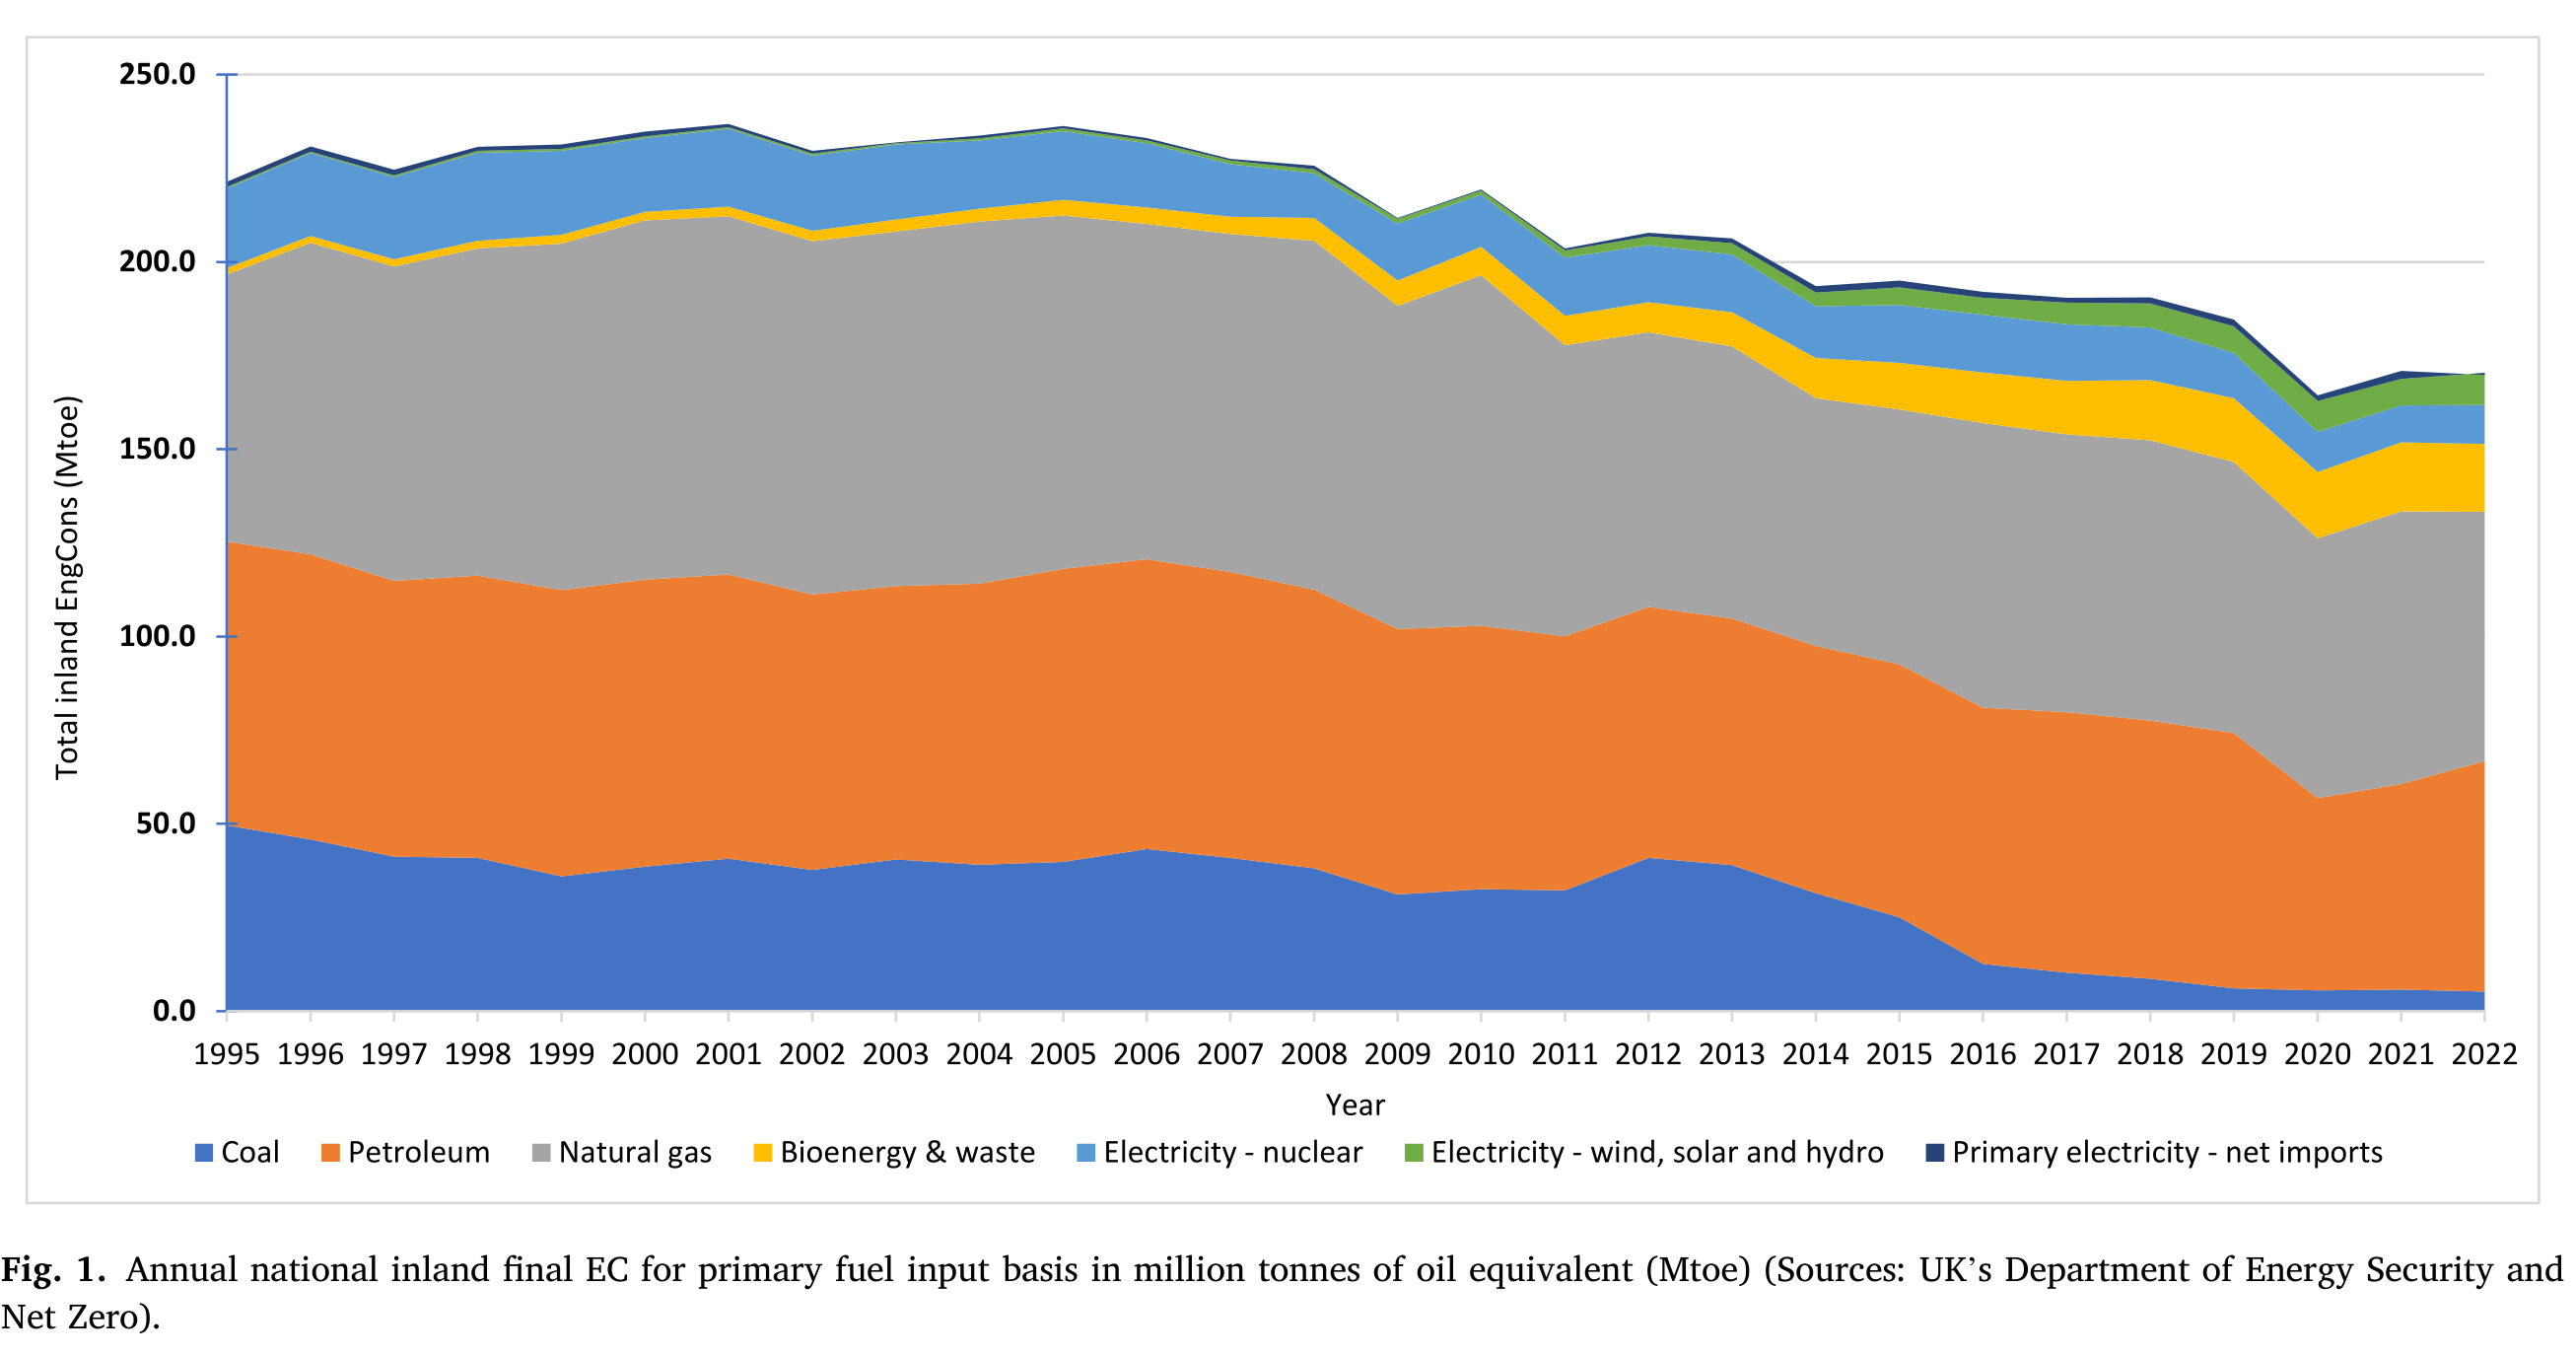
\includegraphics[width=0.96\textwidth,height=0.70\textheight,keepaspectratio]{figures/paper_original/fig01_annual_energy_mix.png}
\caption{Hình 1 trong bài báo gốc: cơ cấu tiêu thụ năng lượng nội địa cuối cùng theo nguồn năng lượng tại Vương quốc Anh. Nguồn: Eskandari et al. [1], tr. 2.}
\label{fig:orig-01}
\end{figure}

\begin{figure}[p]
\centering
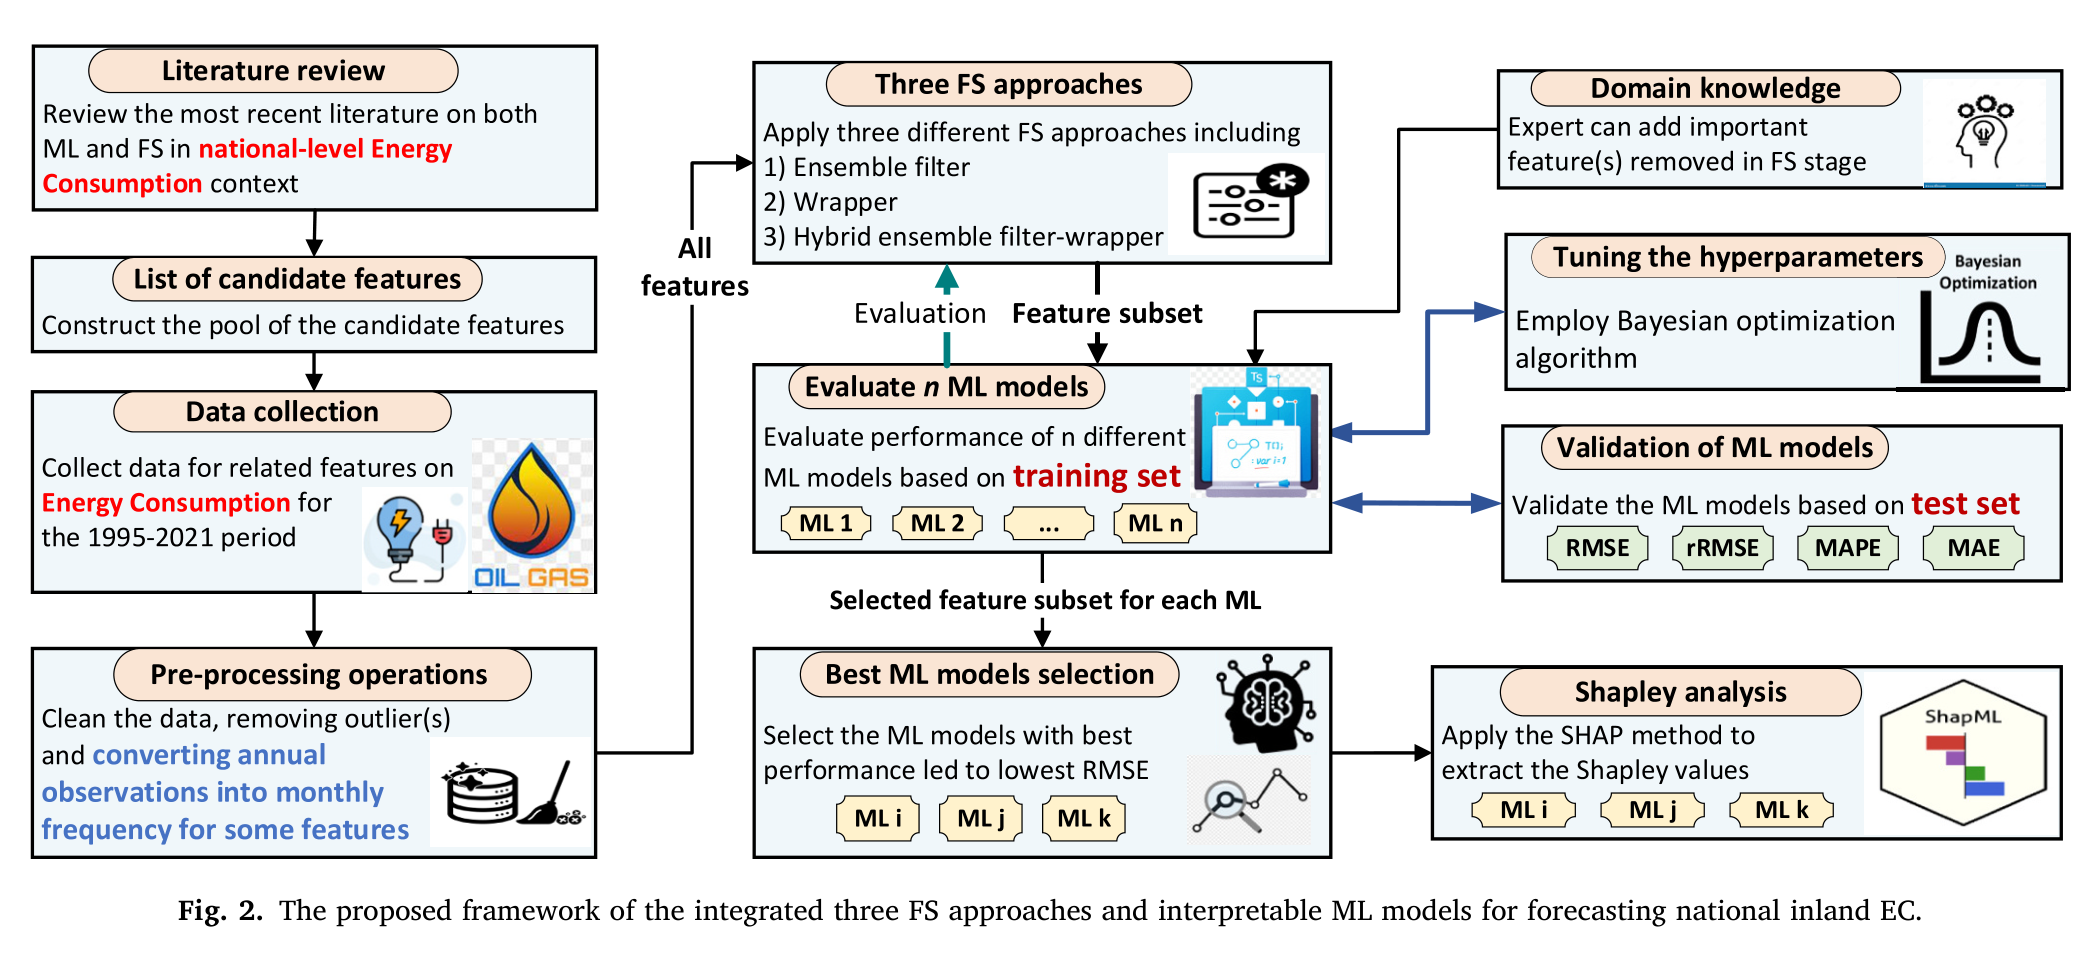
\includegraphics[width=0.98\textwidth,height=0.66\textheight,keepaspectratio]{figures/paper_original/fig02_framework.png}
\caption{Hình 2 trong bài báo gốc: framework tích hợp ba chiến lược Feature Selection, các mô hình ML, Bayesian Optimization, validation và SHAP. Nguồn: [1], tr. 3.}
\label{fig:orig-02}
\end{figure}

\begin{figure}[p]
\centering
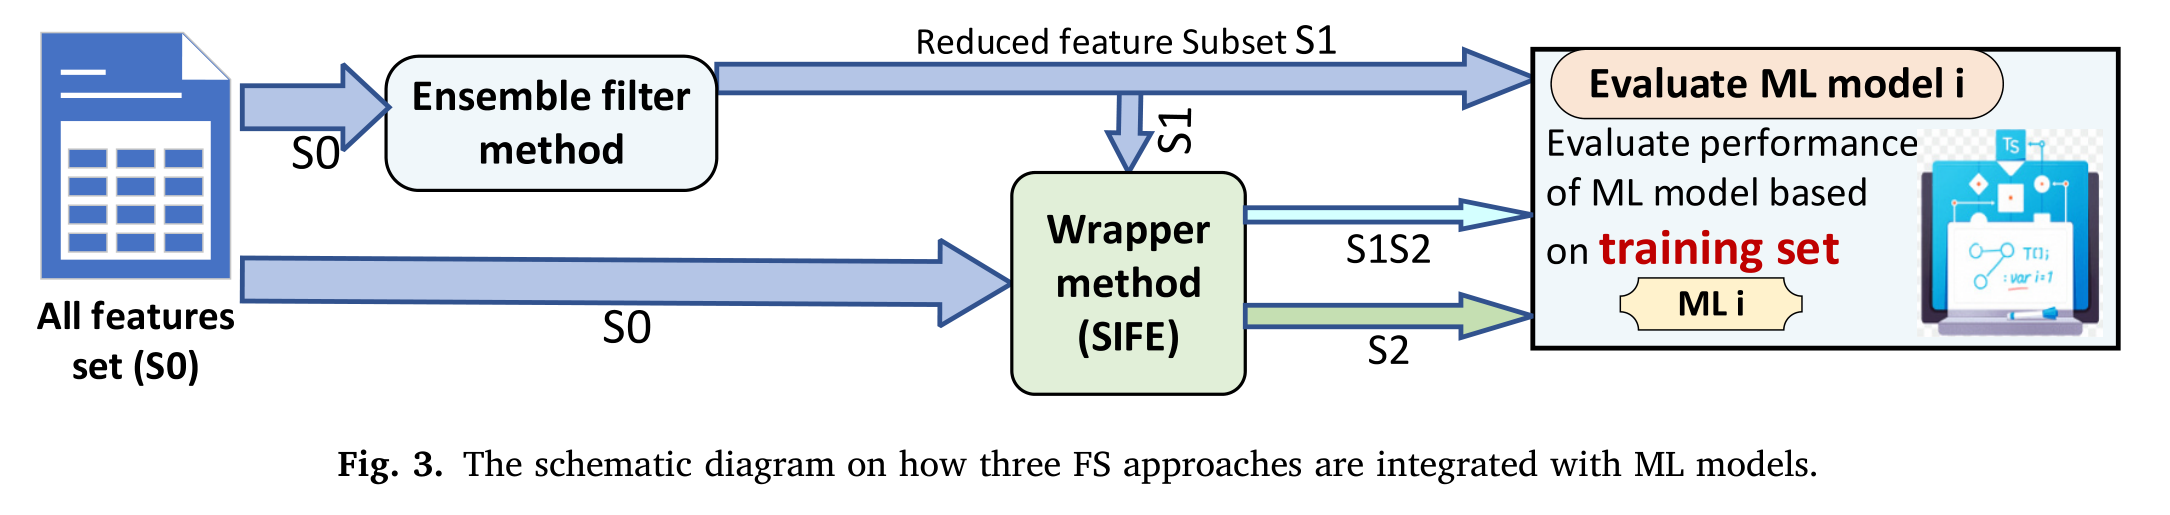
\includegraphics[width=0.98\textwidth,height=0.60\textheight,keepaspectratio]{figures/paper_original/fig03_three_fs_workflow.png}
\caption{Hình 3 trong bài báo gốc: sơ đồ tích hợp ba nhánh S1, S2 và S1S2 với các mô hình ML. Nguồn: [1], tr. 6.}
\label{fig:orig-03}
\end{figure}

\begin{figure}[p]
\centering
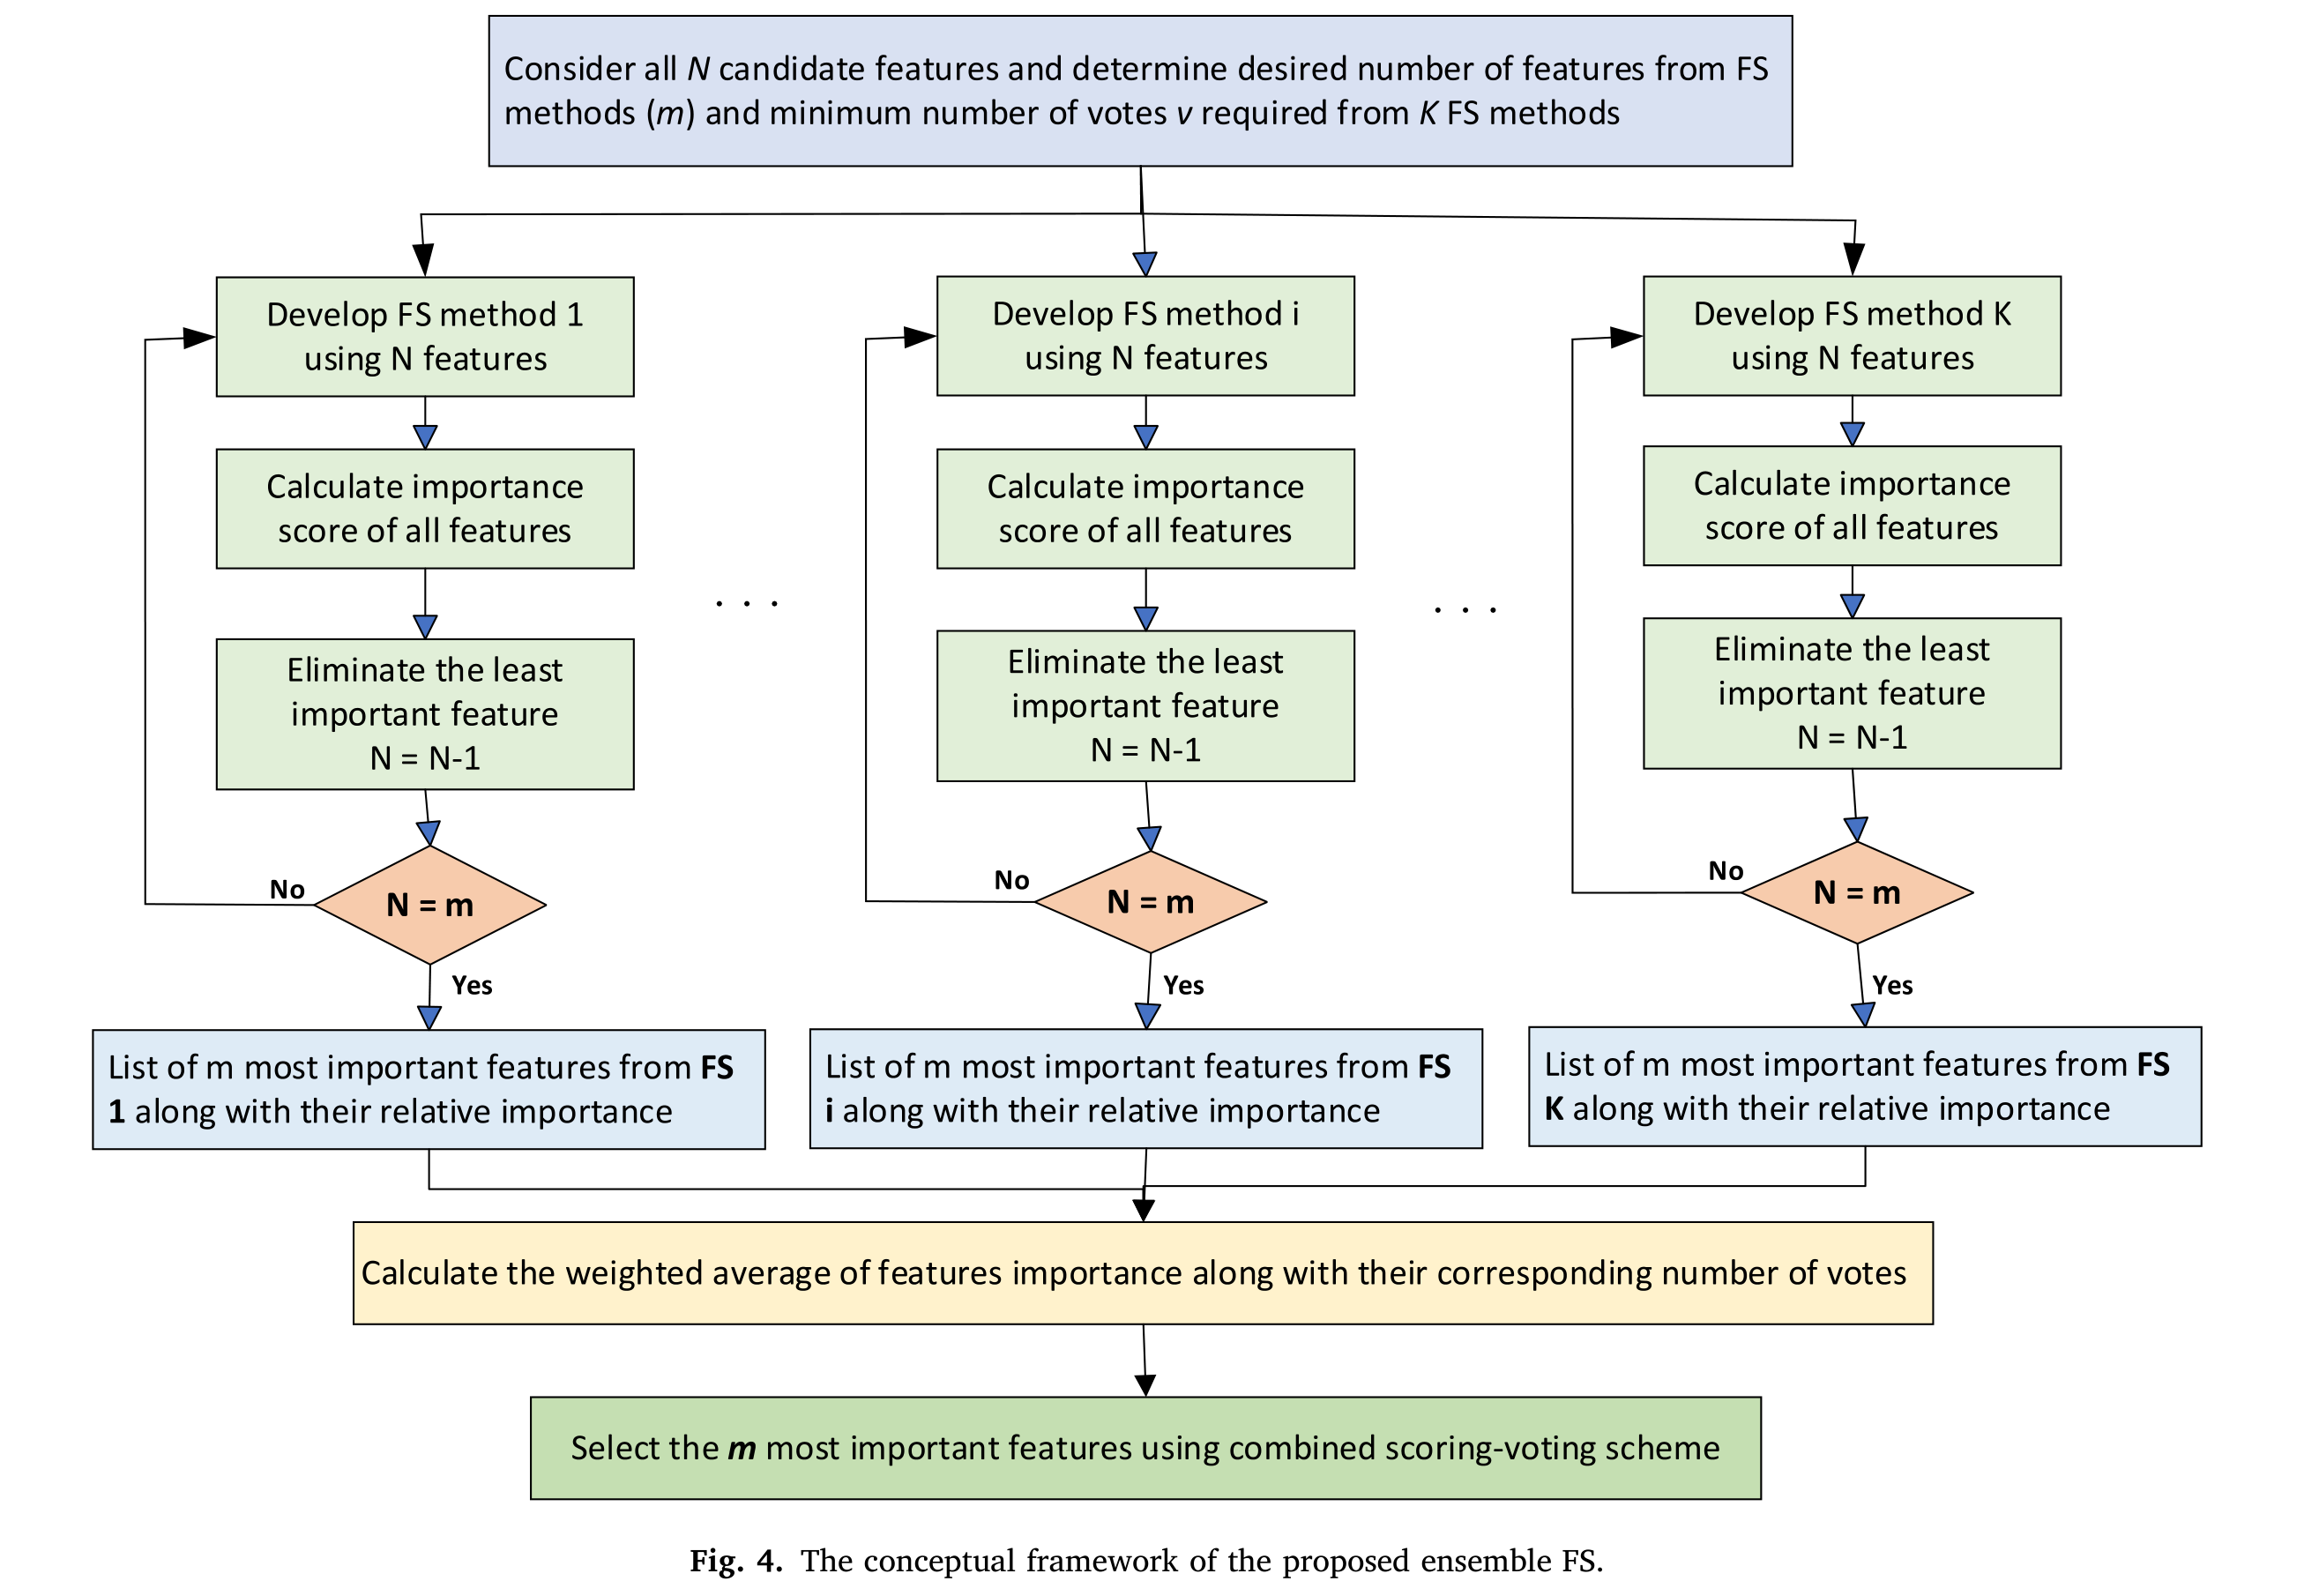
\includegraphics[width=0.98\textwidth,height=0.66\textheight,keepaspectratio]{figures/paper_original/fig04_ensemble_filter.png}
\caption{Hình 4 trong bài báo gốc: quy trình Ensemble Filter với loại dần đặc trưng, tổng hợp importance và voting. Nguồn: [1], tr. 7.}
\label{fig:orig-04}
\end{figure}

\section{Các hình mô tả dữ liệu và phân tích đặc trưng}

\begin{figure}[p]
\centering
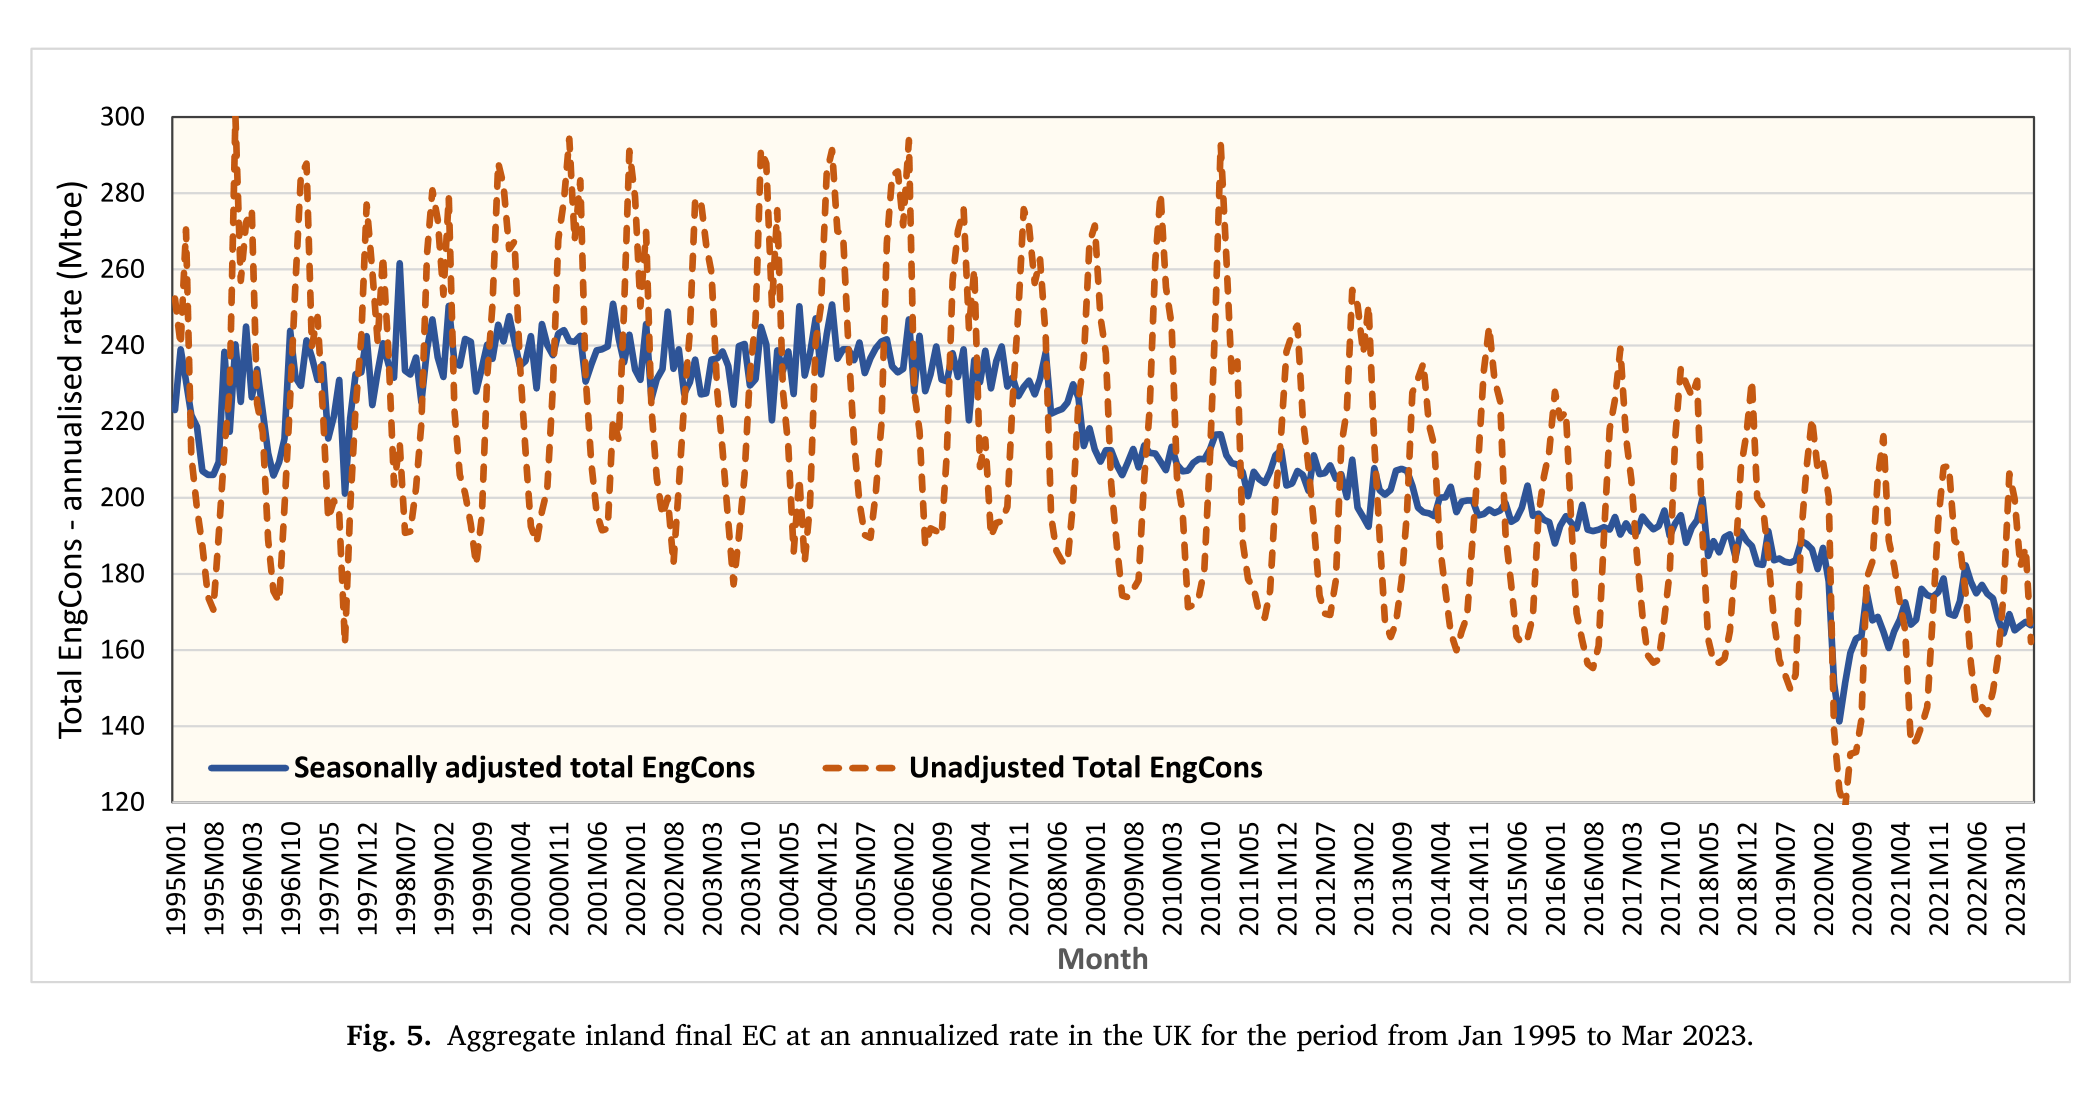
\includegraphics[width=0.98\textwidth,height=0.65\textheight,keepaspectratio]{figures/paper_original/fig05_uk_monthly_ec.png}
\caption{Hình 5 trong bài báo gốc: diễn biến tổng tiêu thụ năng lượng nội địa cuối cùng theo tháng tại Vương quốc Anh. Nguồn: [1], tr. 10.}
\label{fig:orig-05}
\end{figure}

\begin{figure}[p]
\centering
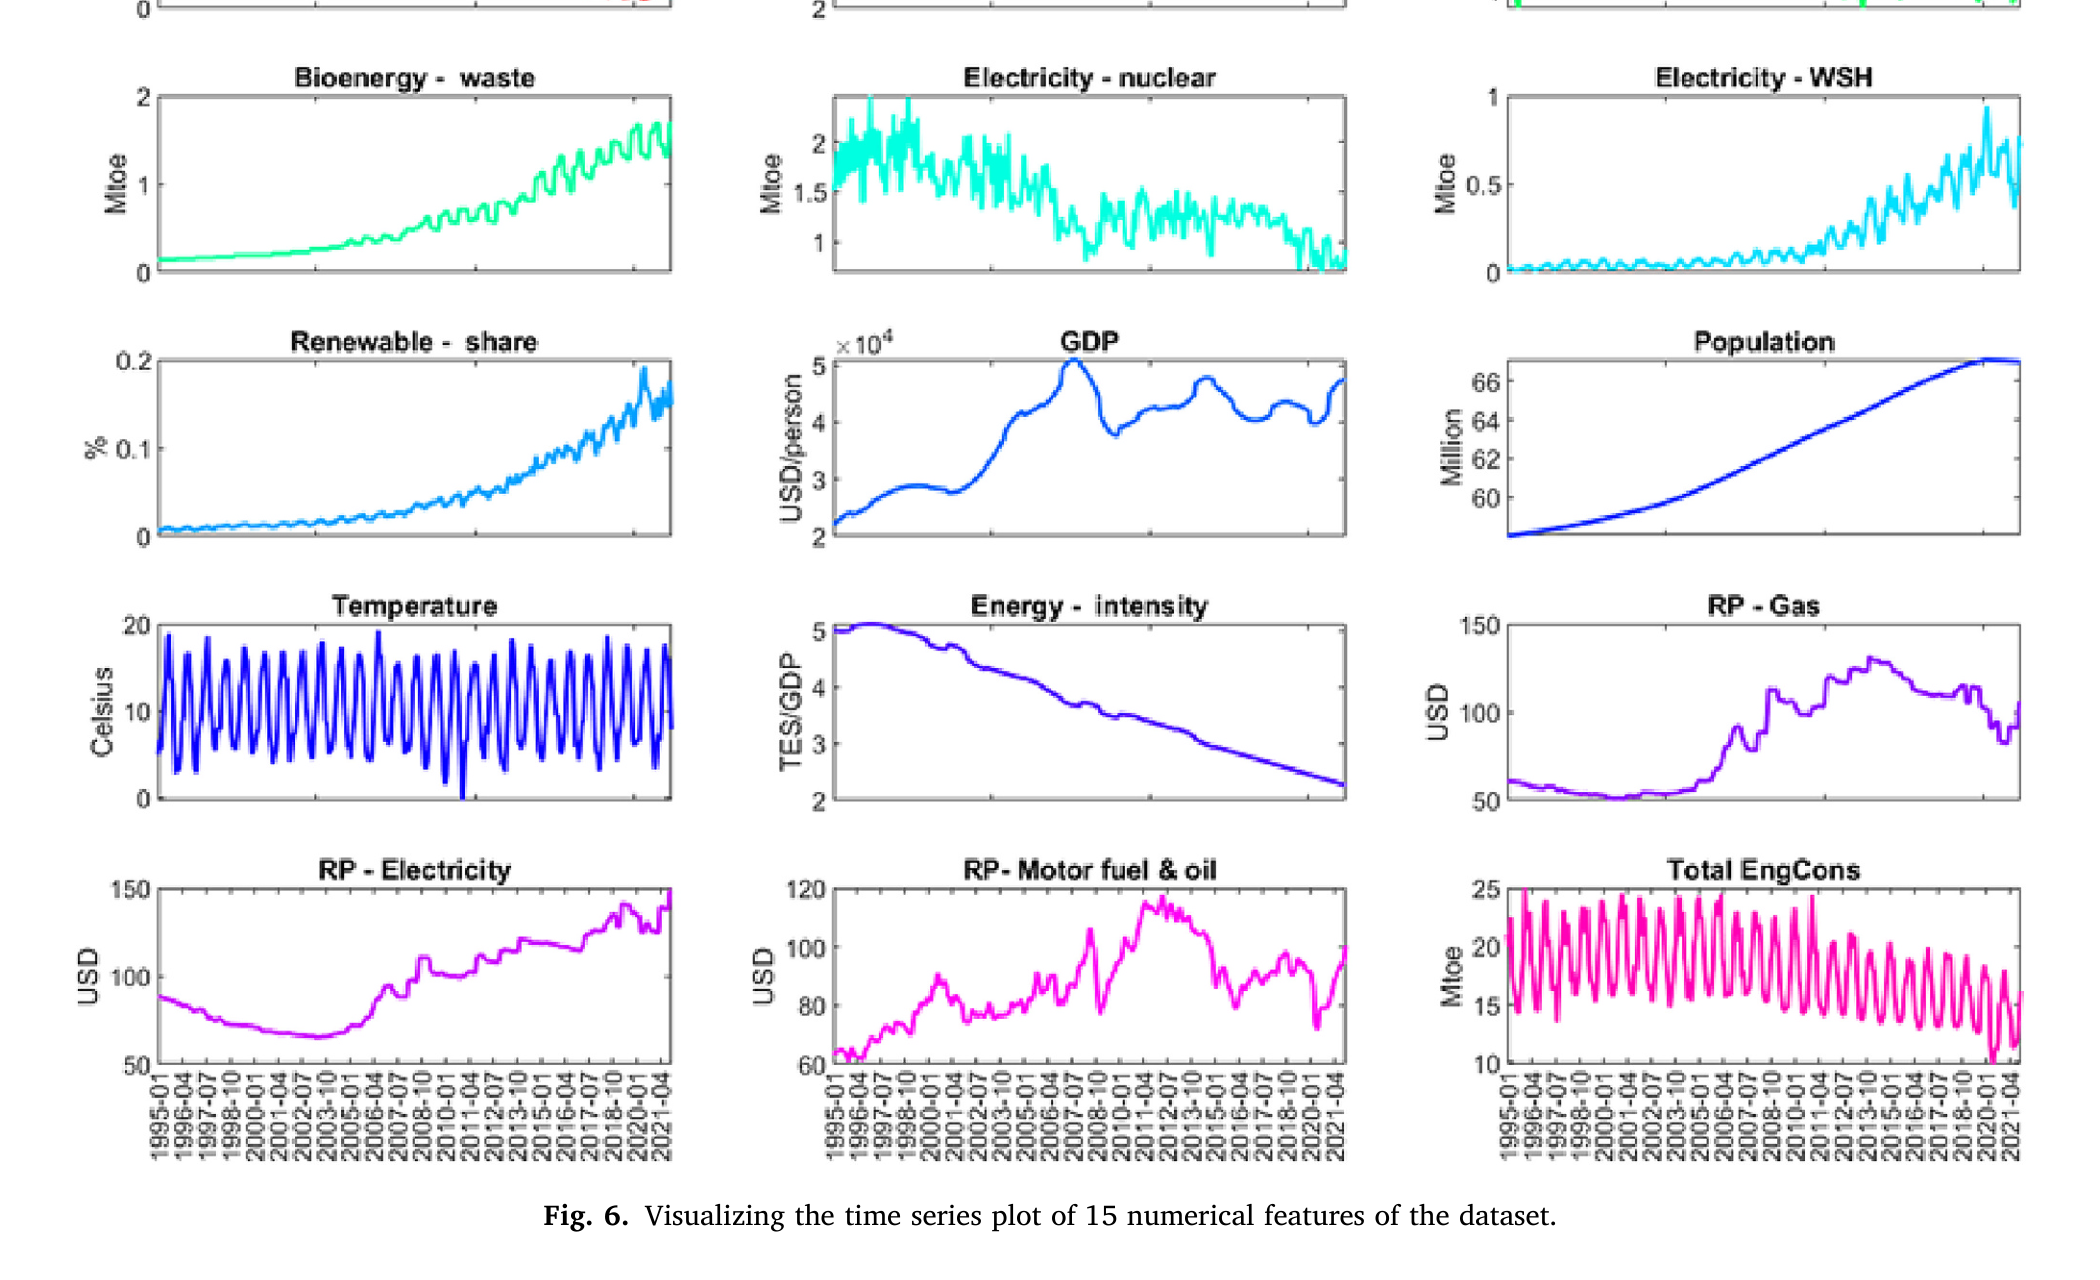
\includegraphics[width=0.98\textwidth,height=0.70\textheight,keepaspectratio]{figures/paper_original/fig06_original_feature_series.png}
\caption{Hình 6 trong bài báo gốc: chuỗi thời gian của 15 biến số chính được sử dụng trong nghiên cứu. Nguồn: [1], tr. 11.}
\label{fig:orig-06}
\end{figure}

\begin{figure}[p]
\centering
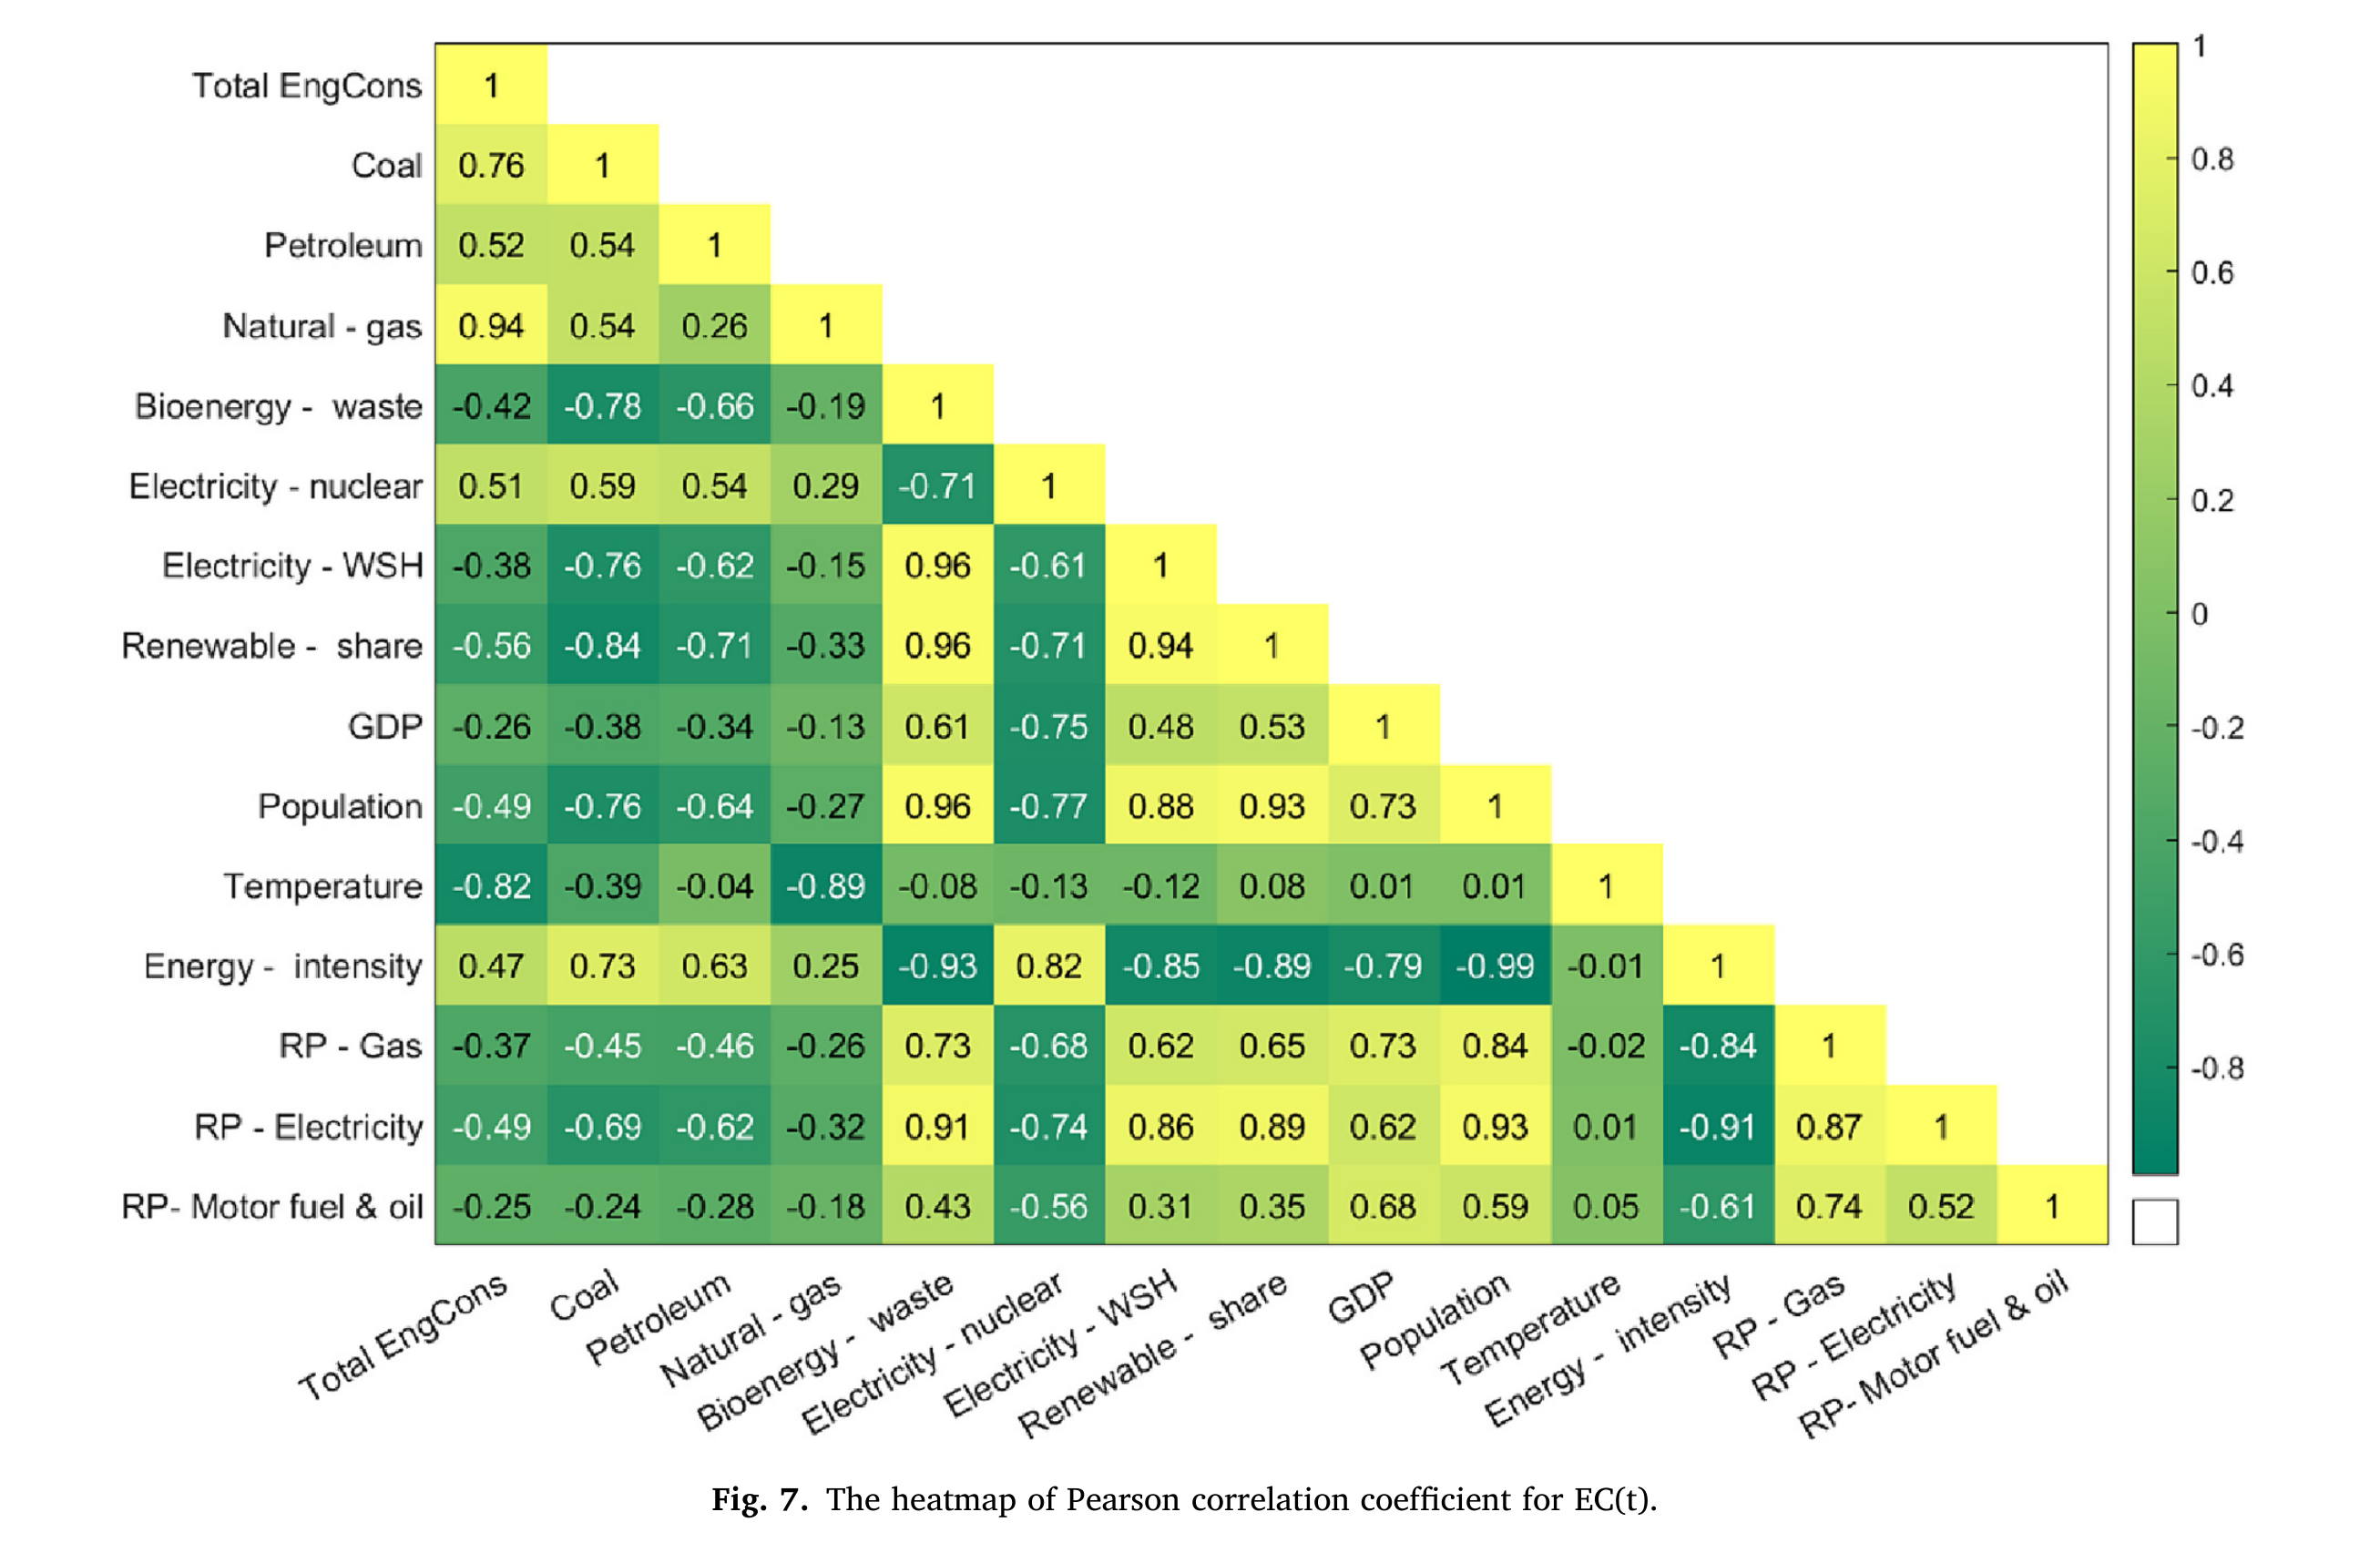
\includegraphics[width=0.98\textwidth,height=0.68\textheight,keepaspectratio]{figures/paper_original/fig07_pearson_heatmap.png}
\caption{Hình 7 trong bài báo gốc: heatmap hệ số tương quan Pearson giữa các biến tiêu thụ năng lượng và biến giải thích. Nguồn: [1], tr. 13.}
\label{fig:orig-07}
\end{figure}

\section{Các hình kết quả dự báo}

\begin{figure}[p]
\centering
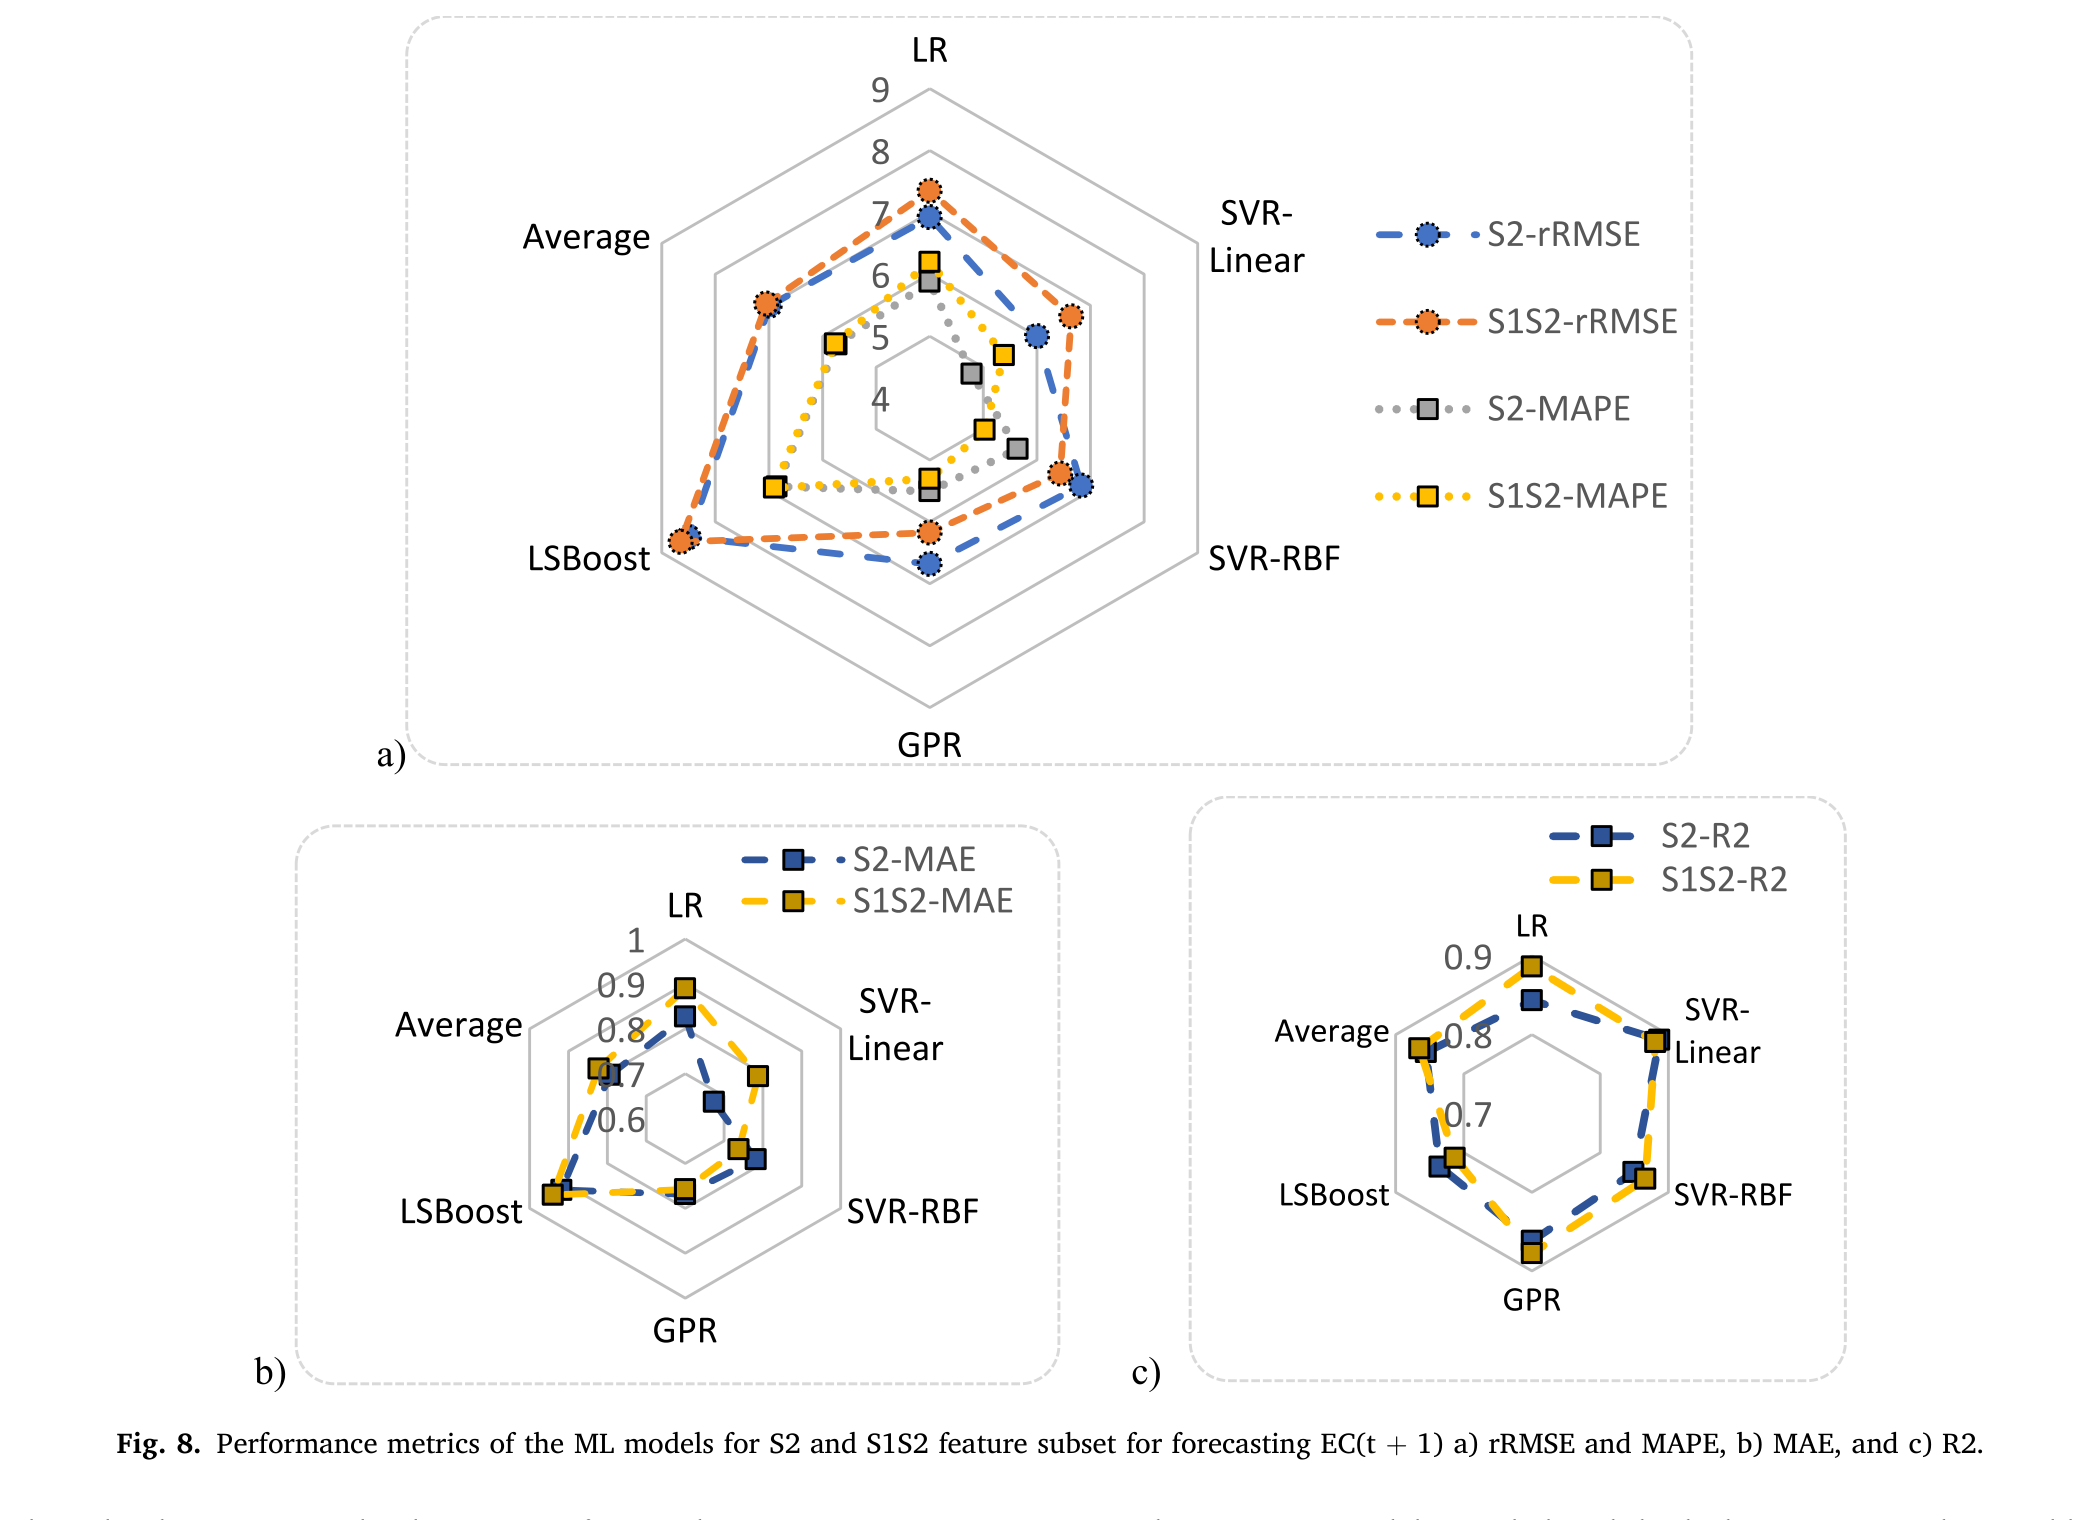
\includegraphics[width=0.98\textwidth,height=0.68\textheight,keepaspectratio]{figures/paper_original/fig08_model_metrics.png}
\caption{Hình 8 trong bài báo gốc: biểu đồ so sánh metric giữa S2 và S1S2. Nguồn: [1], tr. 15.}
\label{fig:orig-08}
\end{figure}

\begin{figure}[p]
\centering
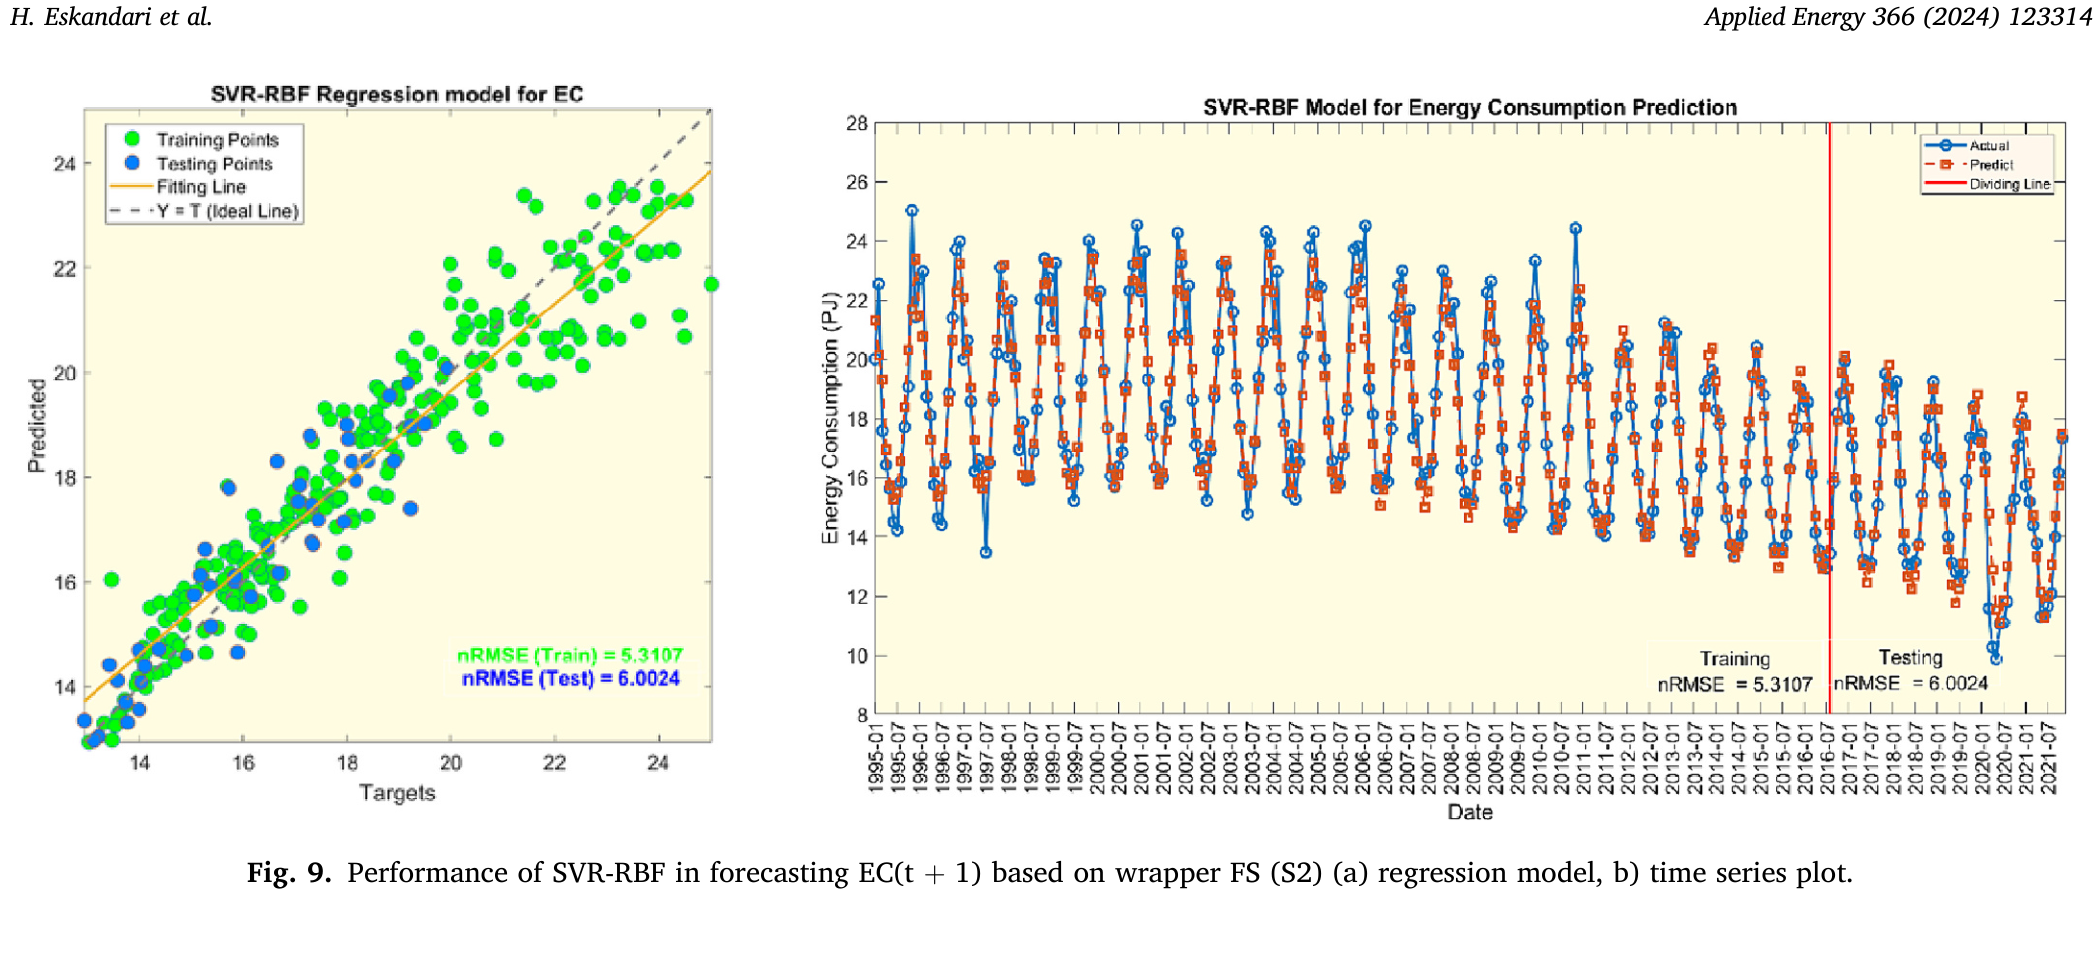
\includegraphics[width=0.98\textwidth,height=0.62\textheight,keepaspectratio]{figures/paper_original/fig09_s2_svr_rbf.png}
\caption{Hình 9 trong bài báo gốc: kết quả SVR-RBF với Wrapper S2, gồm regression plot và chuỗi dự báo. Nguồn: [1], tr. 16.}
\label{fig:orig-09}
\end{figure}

\begin{figure}[p]
\centering
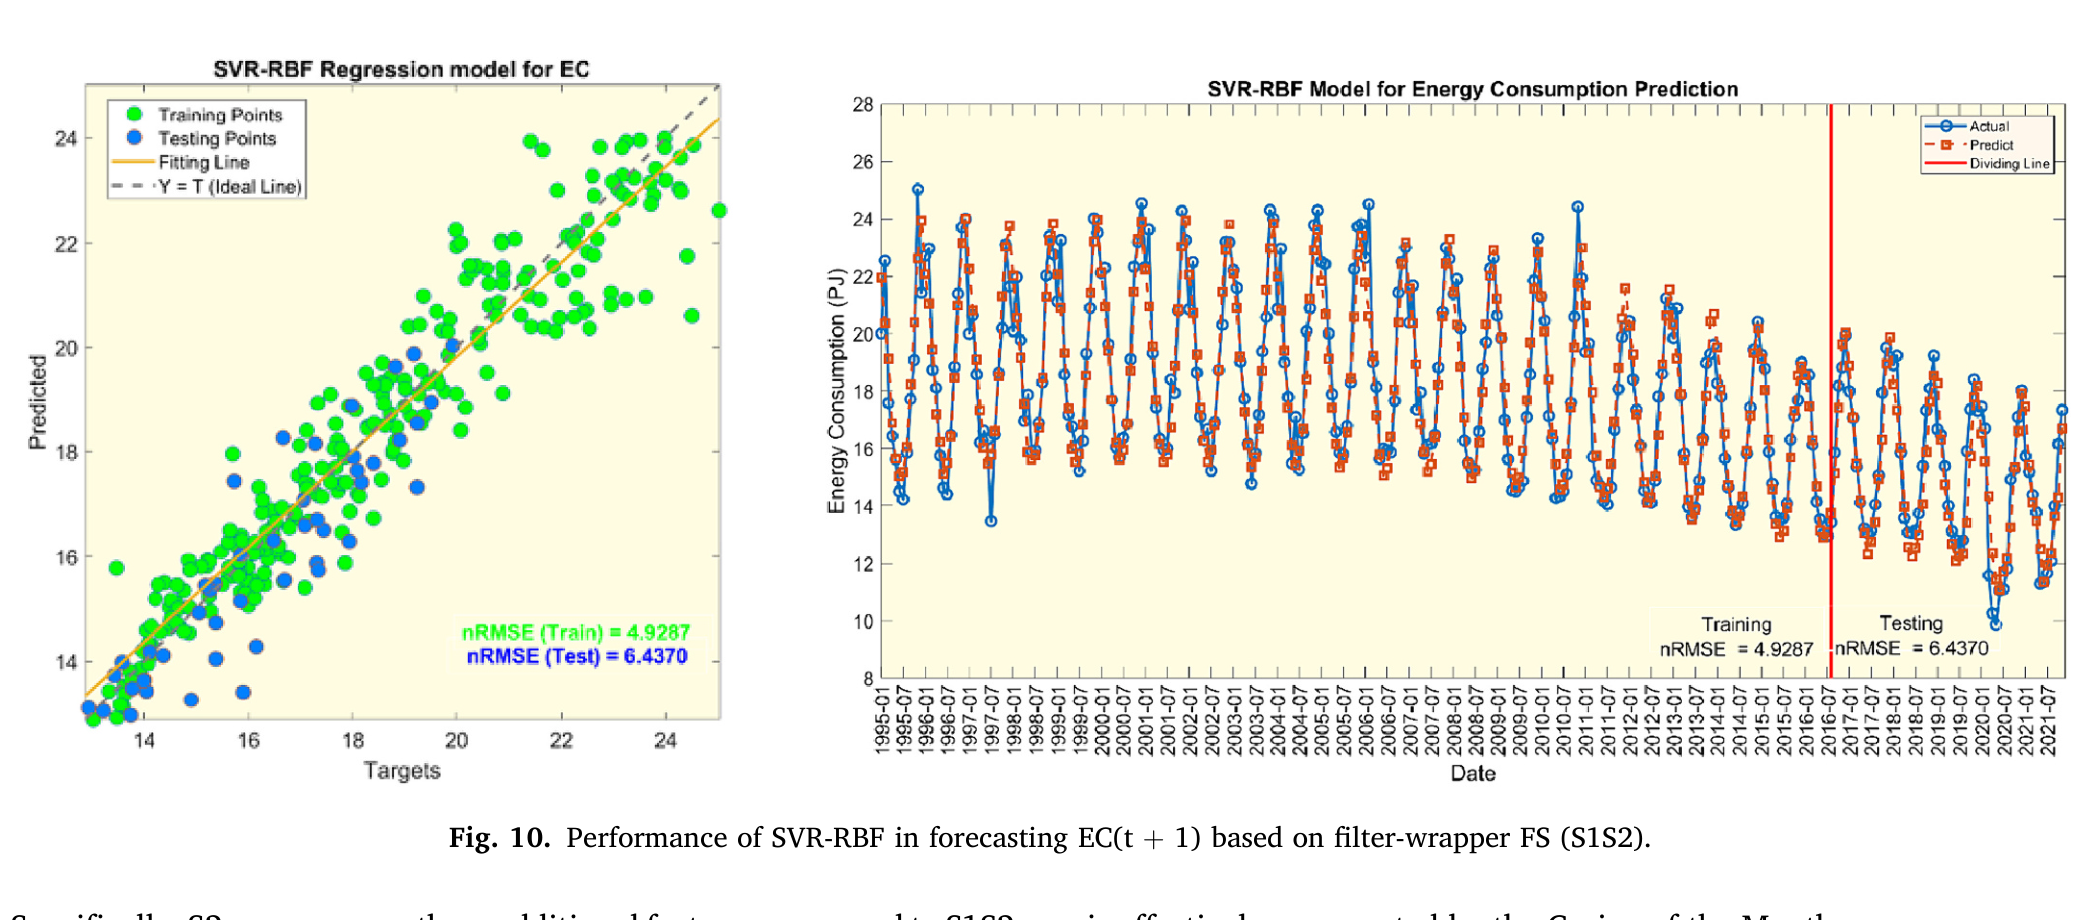
\includegraphics[width=0.98\textwidth,height=0.62\textheight,keepaspectratio]{figures/paper_original/fig10_s1s2_svr_rbf.png}
\caption{Hình 10 trong bài báo gốc: kết quả SVR-RBF với Ensemble Filter-Wrapper S1S2. Nguồn: [1], tr. 16.}
\label{fig:orig-10}
\end{figure}

\section{Các hình SHAP}

\begin{figure}[p]
\centering
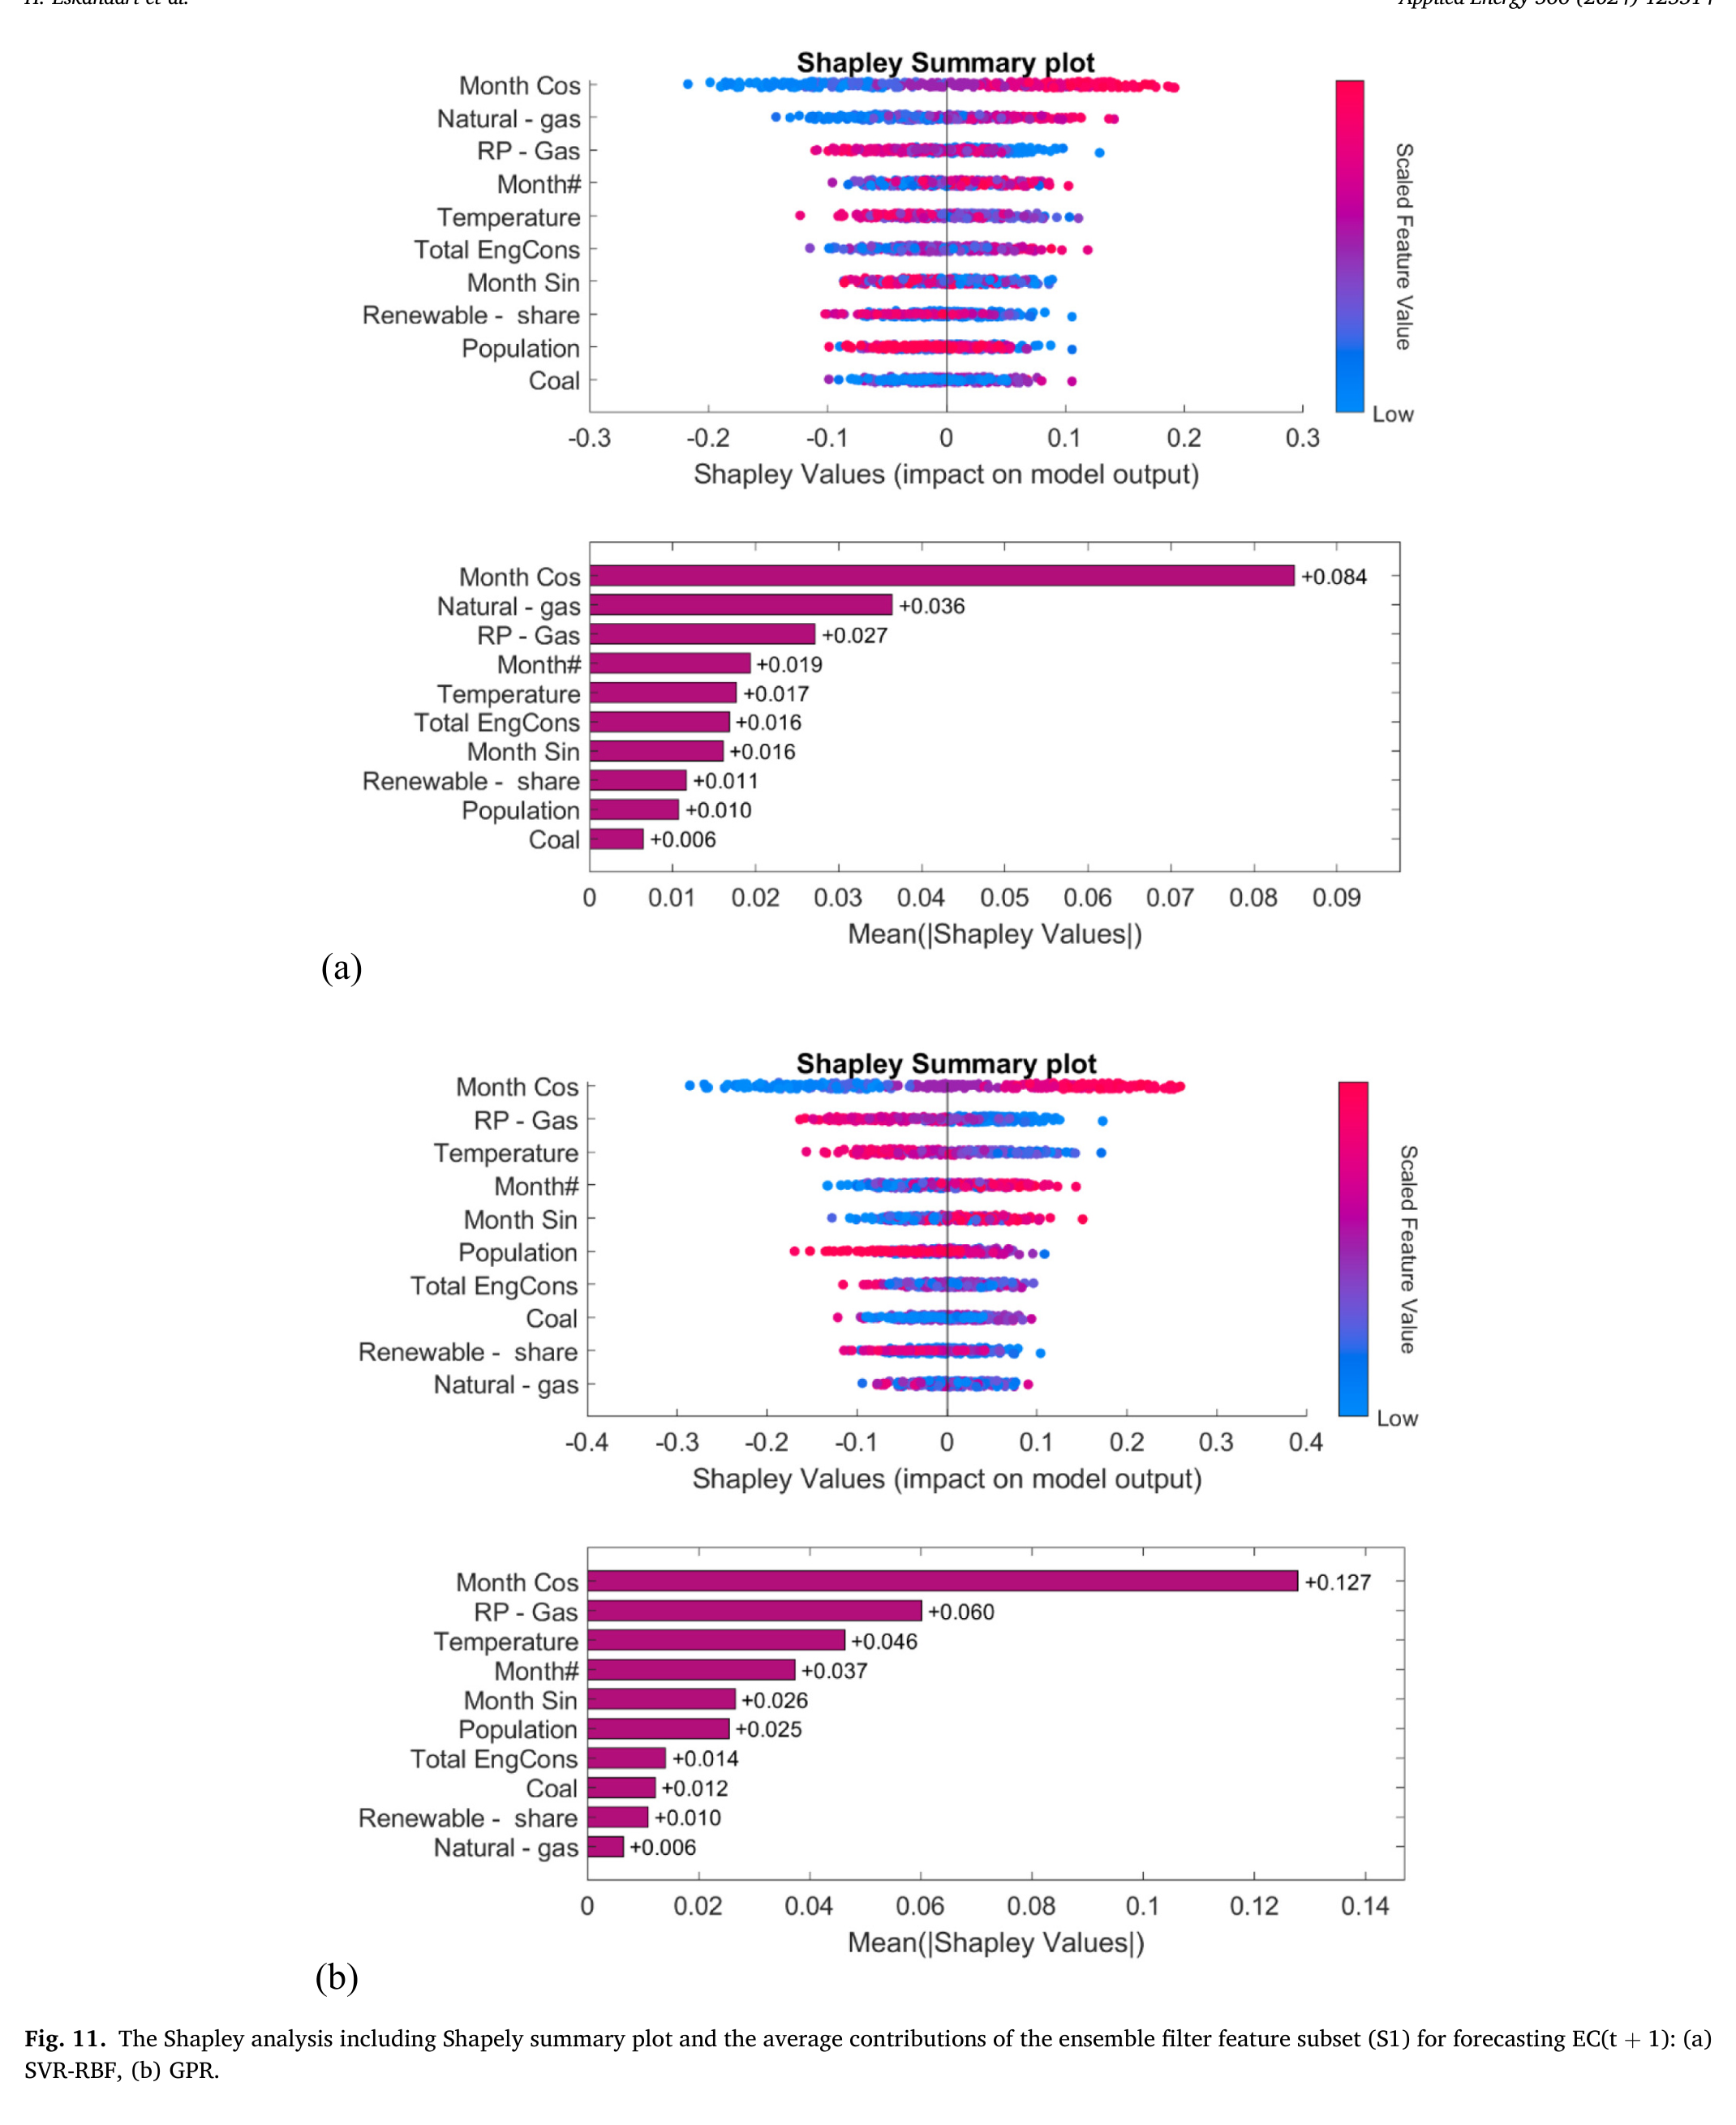
\includegraphics[width=0.88\textwidth,height=0.78\textheight,keepaspectratio]{figures/paper_original/fig11_shap_s1.png}
\caption{Hình 11 trong bài báo gốc: SHAP summary và Mean absolute SHAP của S1 với SVR-RBF và GPR. Nguồn: [1], tr. 17.}
\label{fig:orig-11}
\end{figure}

\begin{figure}[p]
\centering
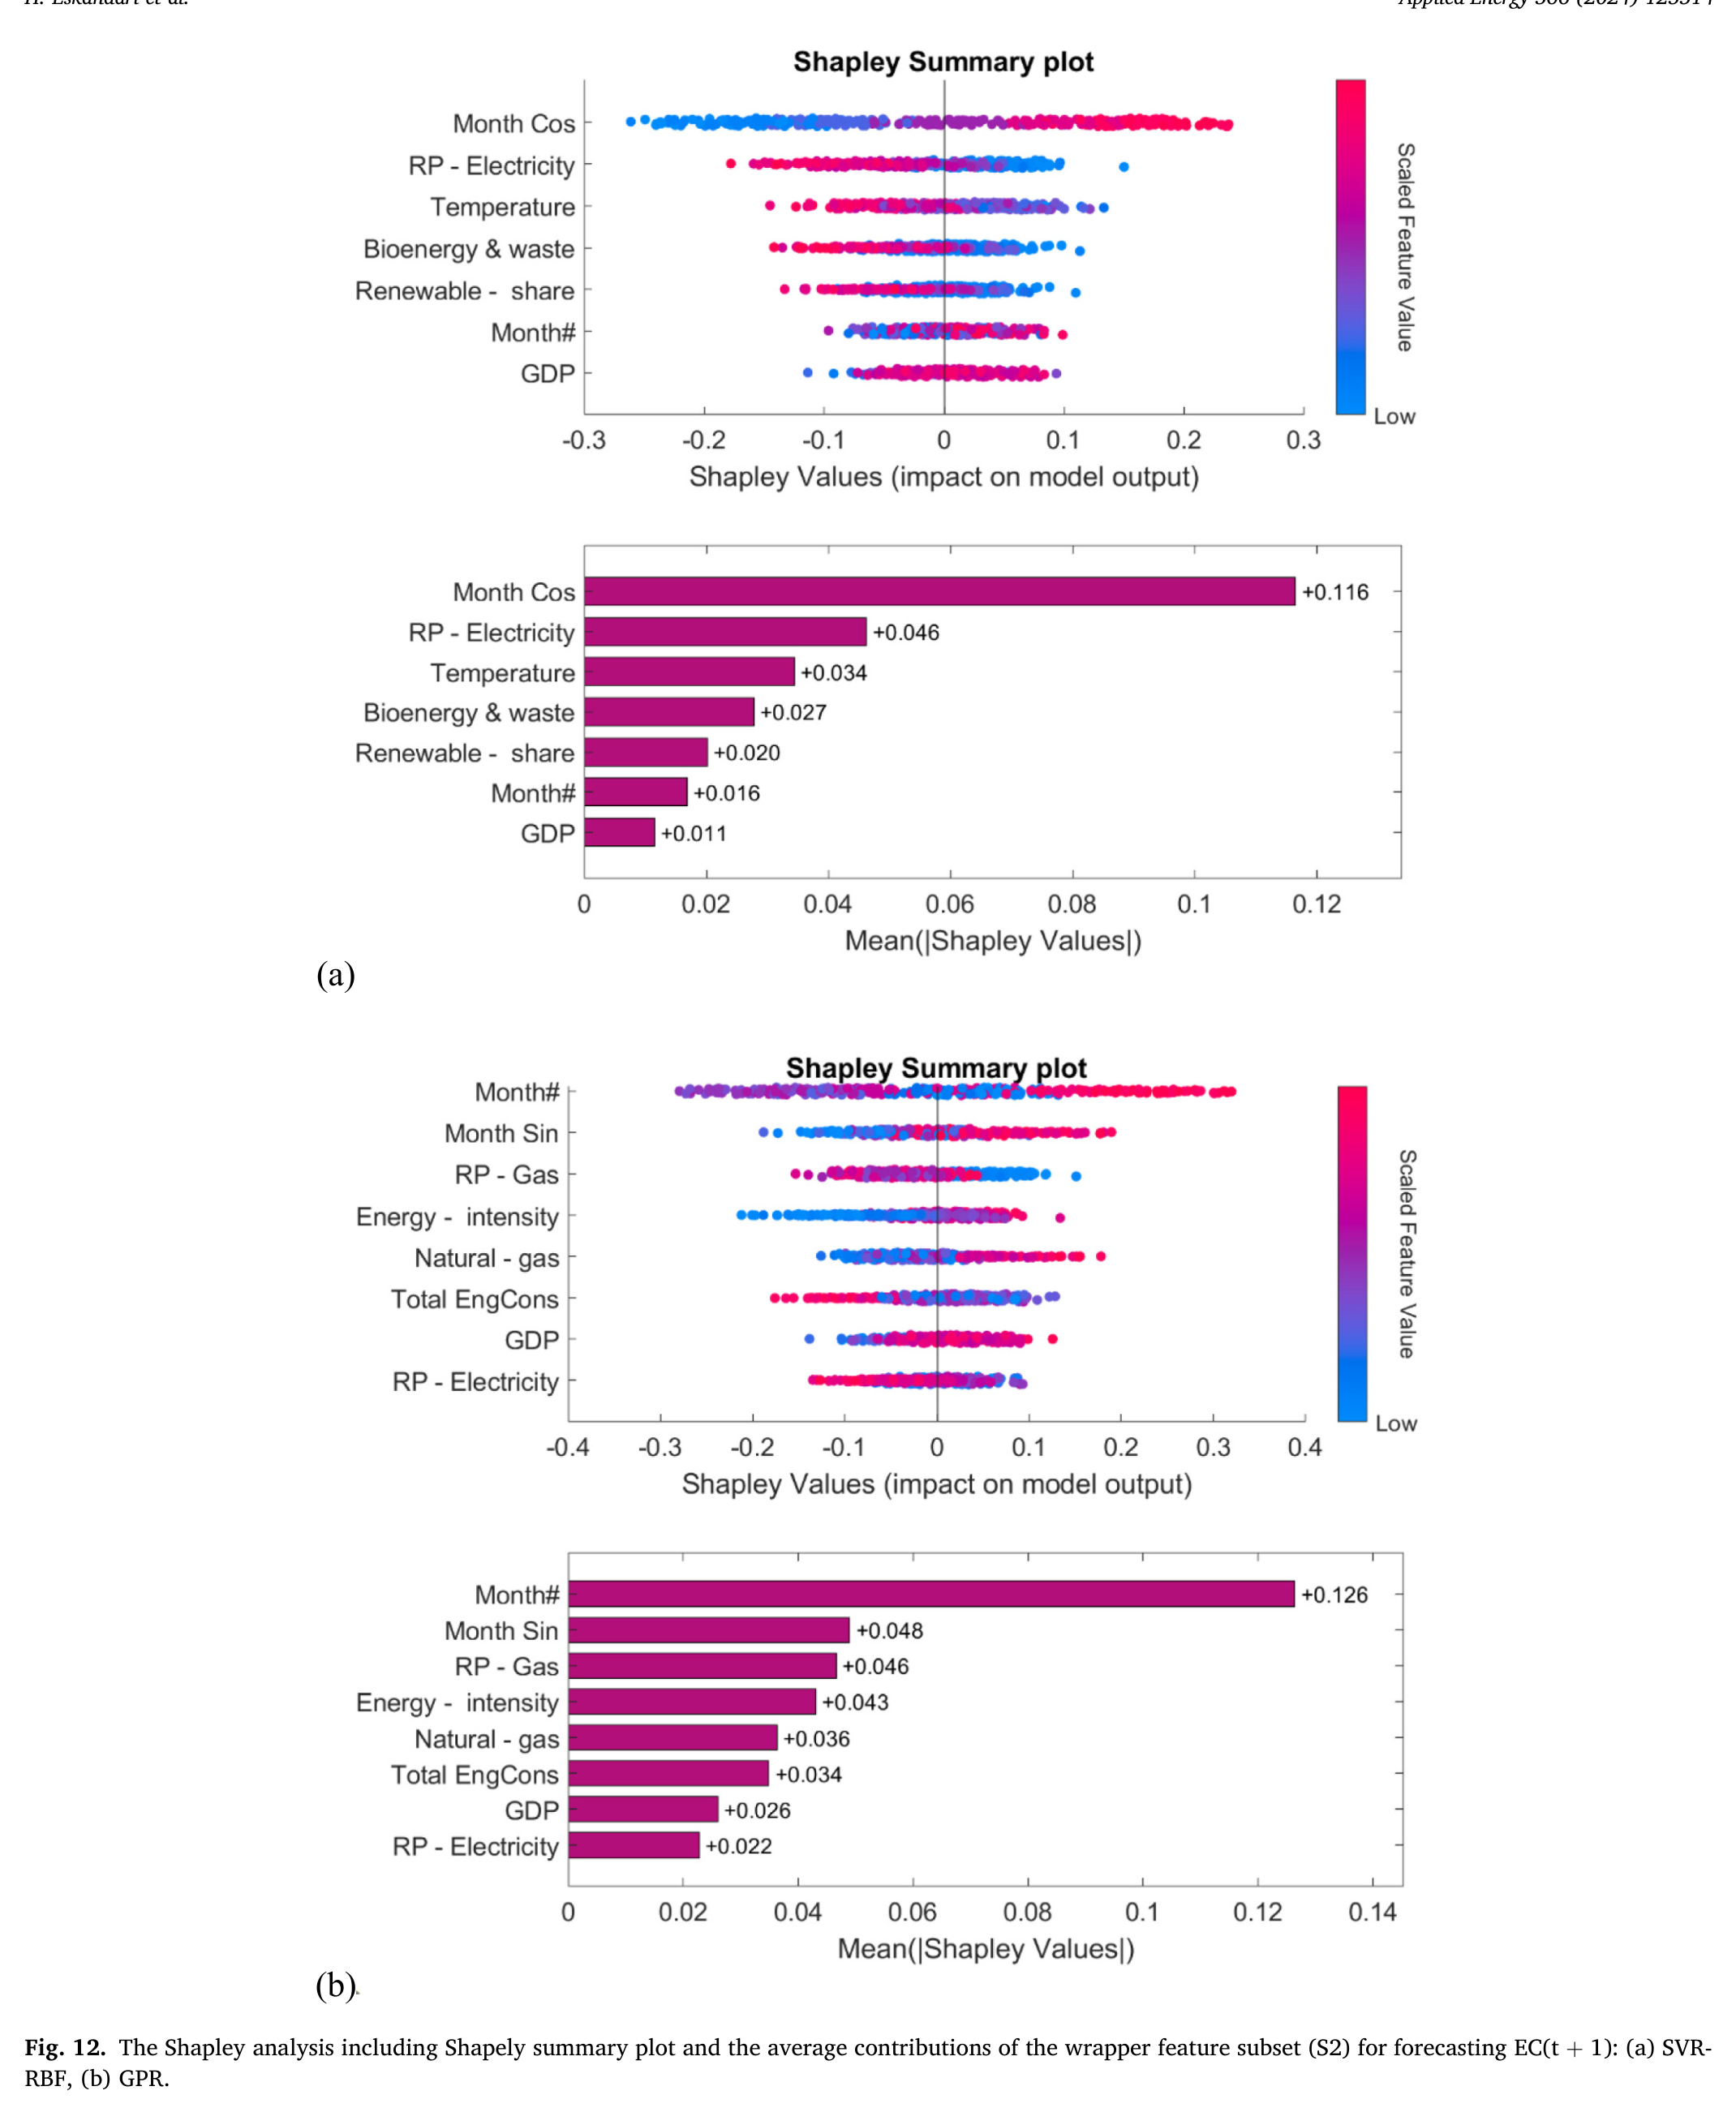
\includegraphics[width=0.88\textwidth,height=0.78\textheight,keepaspectratio]{figures/paper_original/fig12_shap_s2.png}
\caption{Hình 12 trong bài báo gốc: SHAP summary và Mean absolute SHAP của S2 với SVR-RBF và GPR. Nguồn: [1], tr. 18.}
\label{fig:orig-12}
\end{figure}

\begin{figure}[p]
\centering
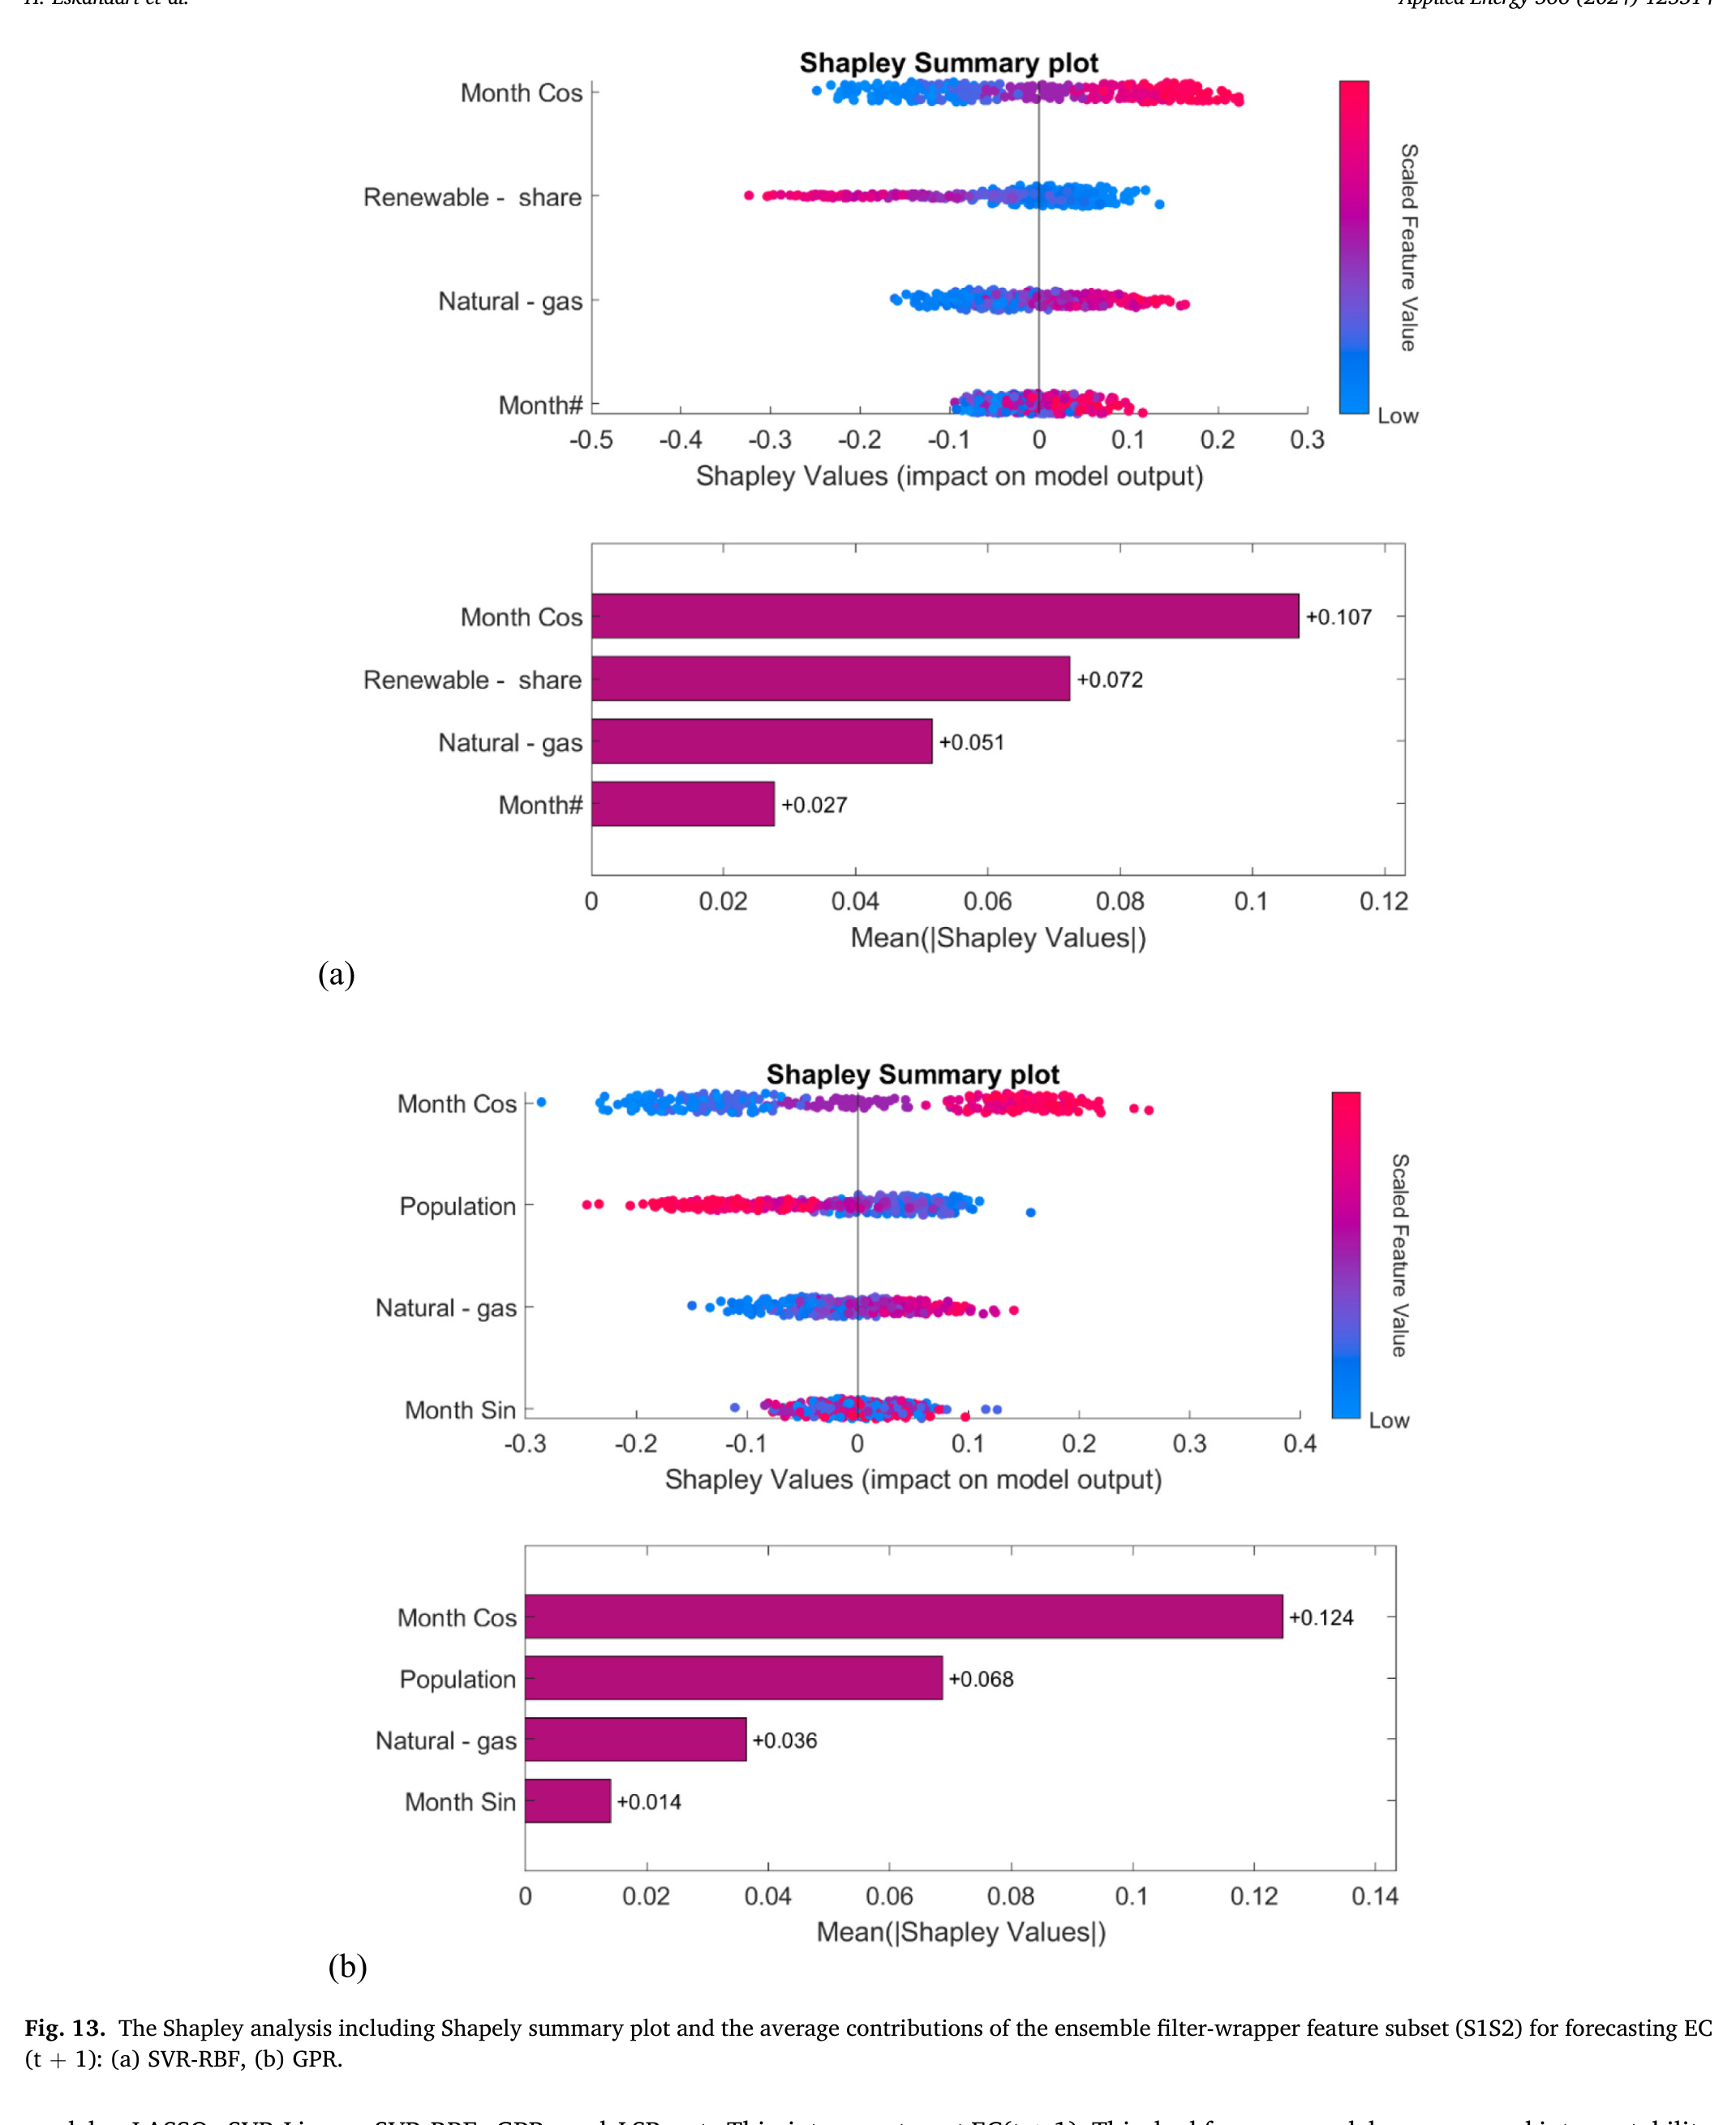
\includegraphics[width=0.88\textwidth,height=0.78\textheight,keepaspectratio]{figures/paper_original/fig13_shap_s1s2.png}
\caption{Hình 13 trong bài báo gốc: SHAP summary và Mean absolute SHAP của S1S2 với SVR-RBF và GPR. Nguồn: [1], tr. 19.}
\label{fig:orig-13}
\end{figure}

\section{Bản trích nguyên gốc các bảng Feature Selection và forecasting}

\begin{landscape}
\begin{table}[p]
\centering
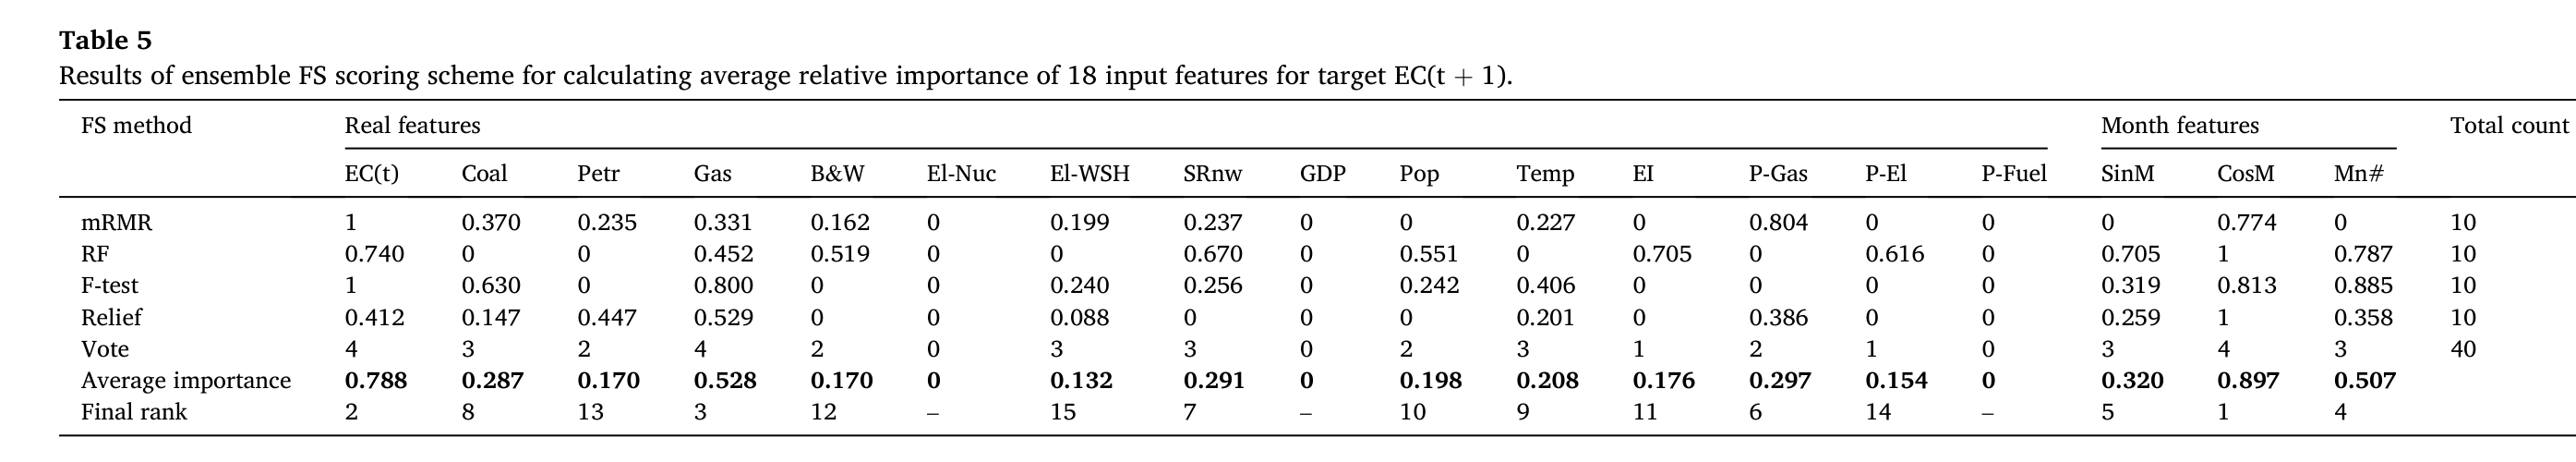
\includegraphics[width=0.96\linewidth,height=0.62\textheight,keepaspectratio]{figures/paper_original/table_5_original.png}
\caption{Bản trích nguyên gốc Table 5: điểm và thứ hạng Ensemble Filter cho 18 đặc trưng. Nguồn: [1], tr. 14.}
\label{tab:orig-5-image}
\end{table}
\end{landscape}

\begin{landscape}
\begin{table}[p]
\centering
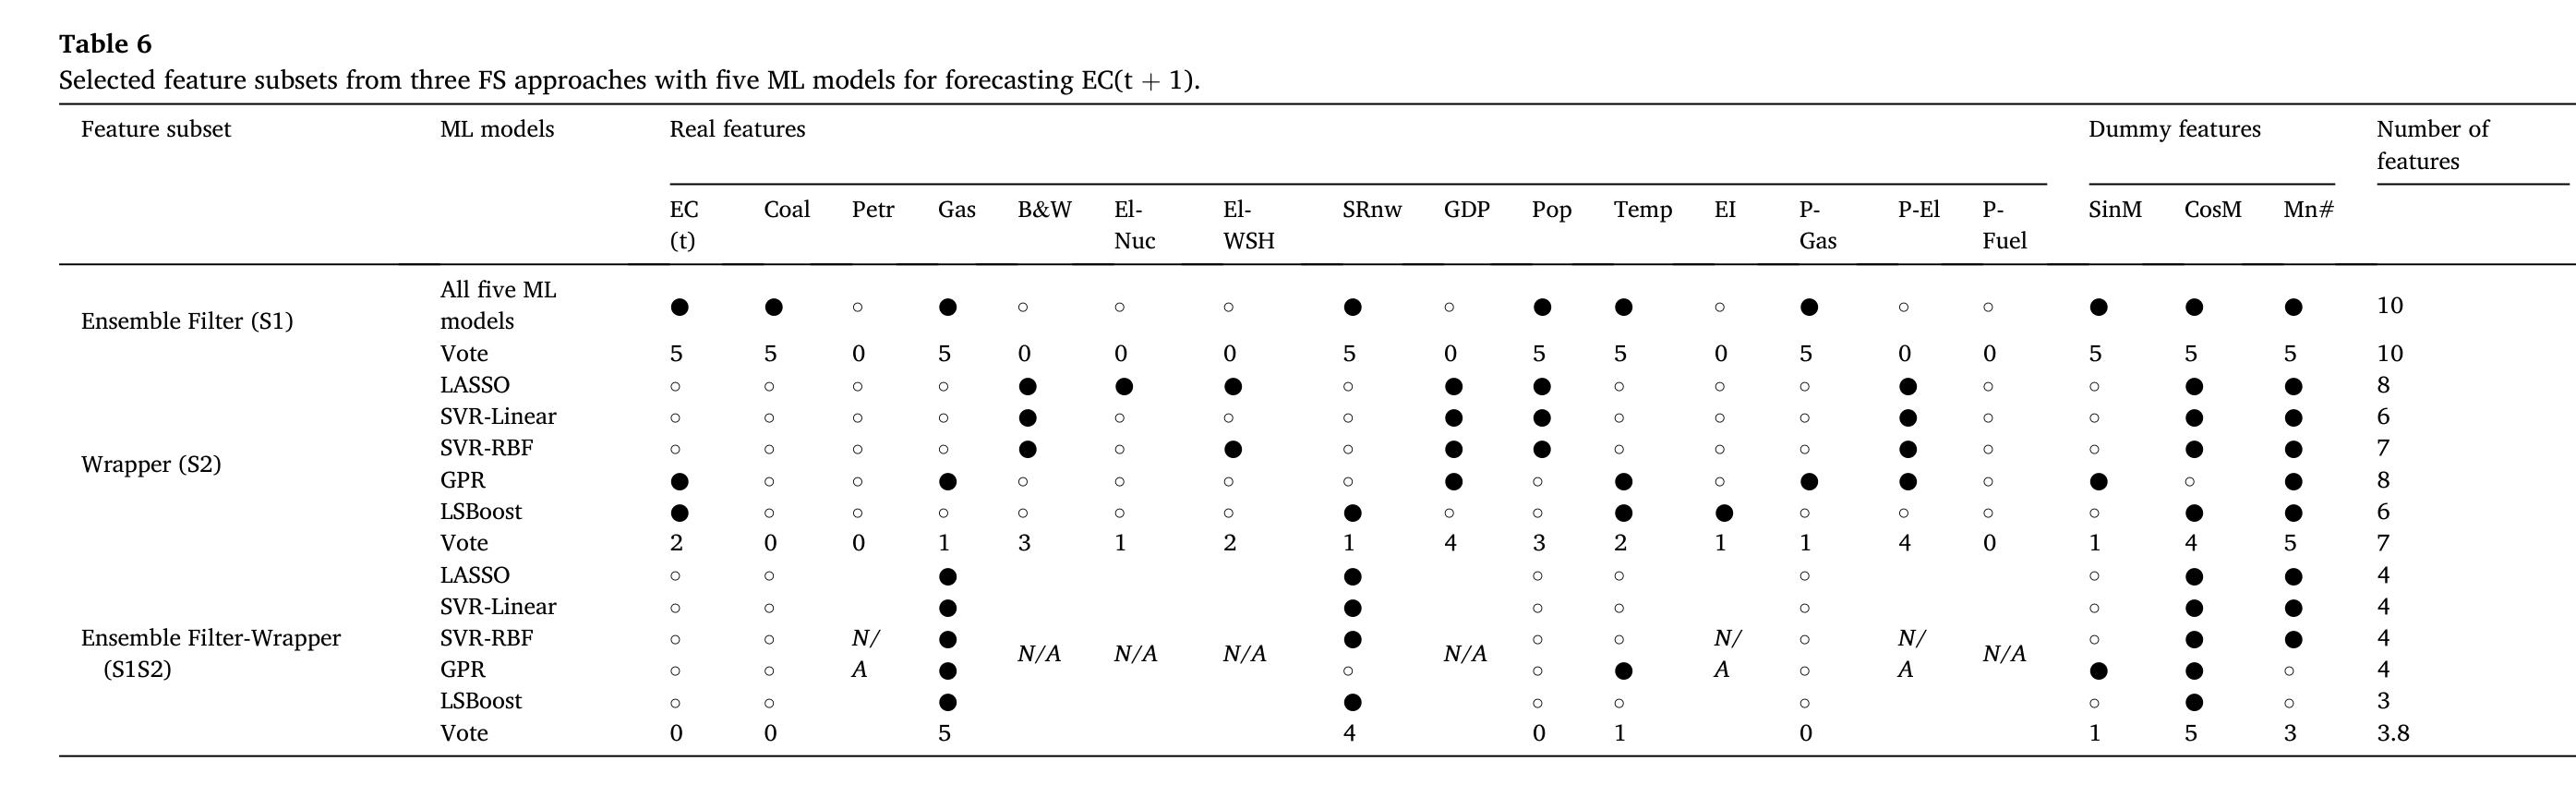
\includegraphics[width=0.96\linewidth,height=0.72\textheight,keepaspectratio]{figures/paper_original/table_6_original.png}
\caption{Bản trích nguyên gốc Table 6: các tập đặc trưng S1, S2 và S1S2 theo từng ML model. Nguồn: [1], tr. 14.}
\label{tab:orig-6-image}
\end{table}
\end{landscape}

\begin{landscape}
\begin{table}[p]
\centering
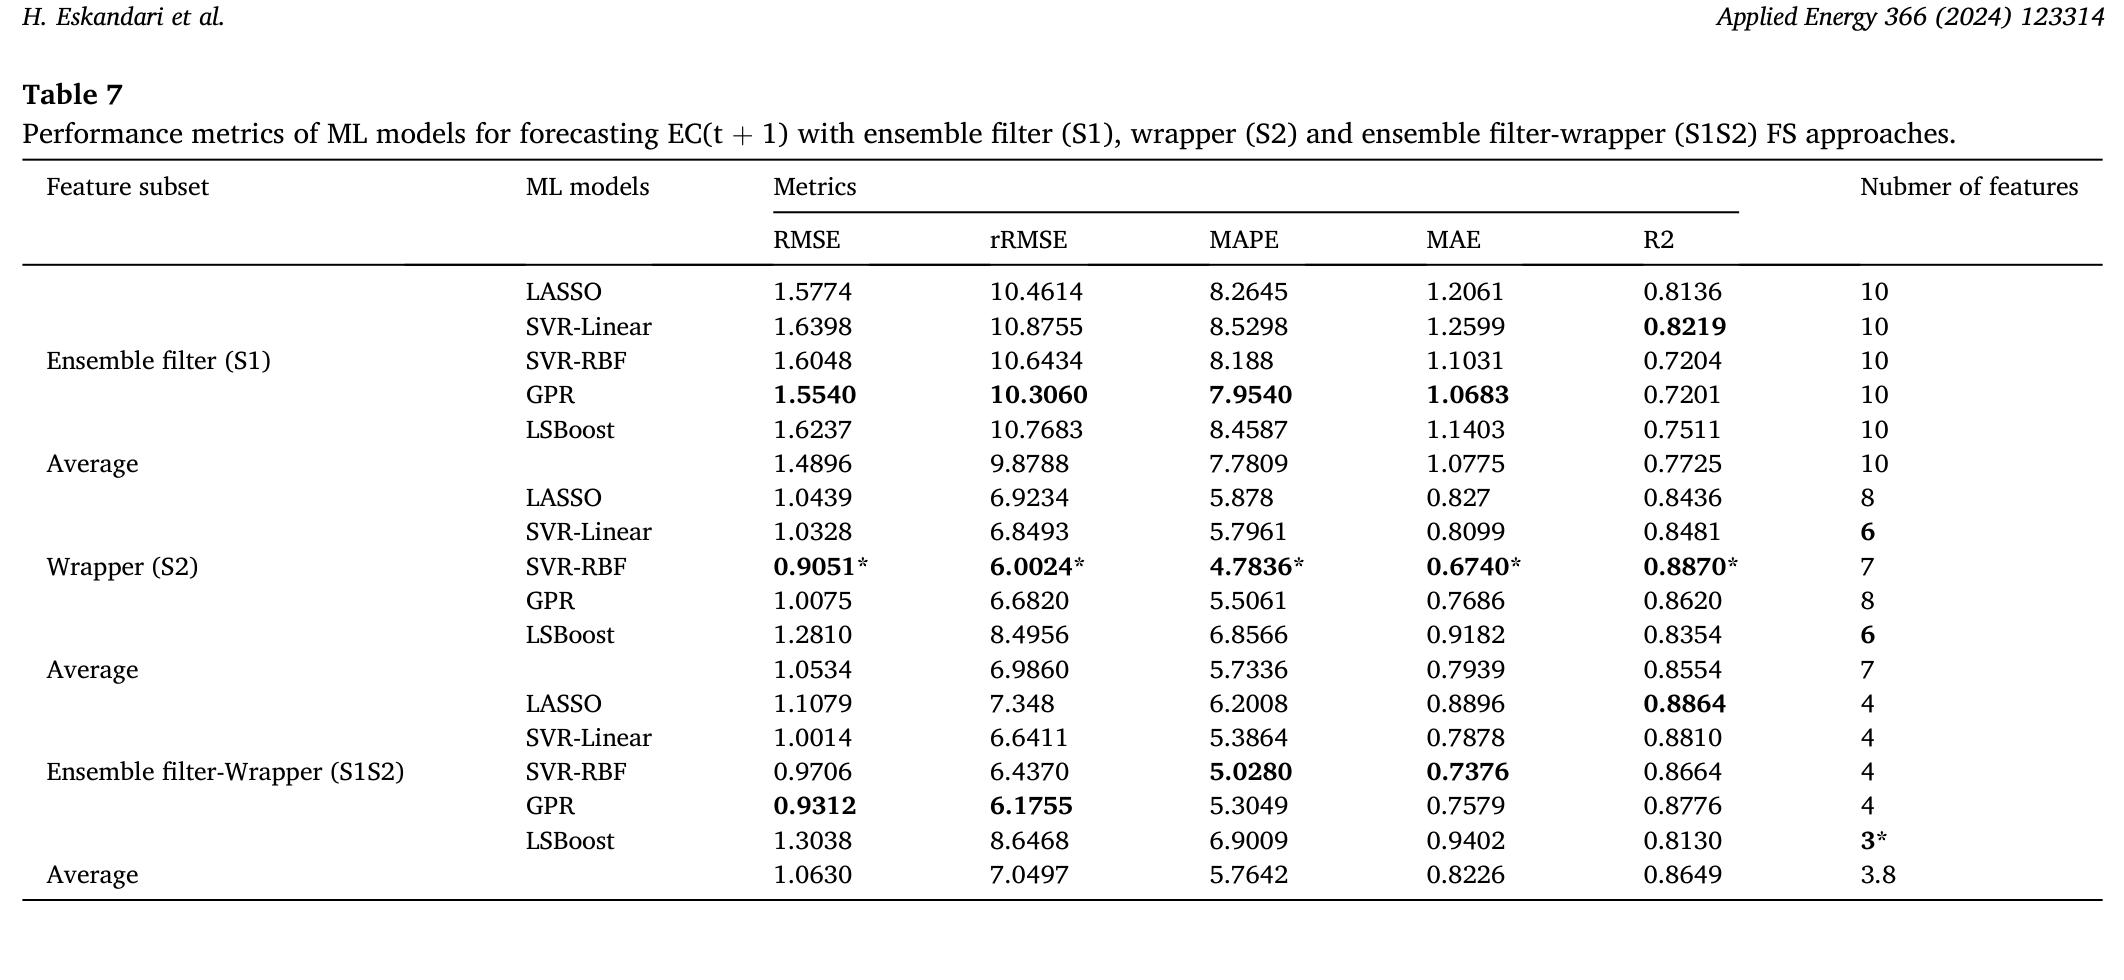
\includegraphics[width=0.96\linewidth,height=0.72\textheight,keepaspectratio]{figures/paper_original/table_7_original.png}
\caption{Bản trích nguyên gốc Table 7: các metric dự báo của 15 cấu hình S1, S2 và S1S2. Nguồn: [1], tr. 15.}
\label{tab:orig-7-image}
\end{table}
\end{landscape}

\noindent Các bảng số liệu có thể đọc và trích dẫn trong nội dung chính được trình bày lại dưới dạng bảng LaTeX tại Chương 5. Ảnh nguồn trong phụ lục được giữ để người đọc có thể kiểm tra cách trình bày ban đầu của tác giả.

\end{document}
